\startchapter{A one-dimensional model of RO membrane scaling via ROSSpy}

\section{Introduction}
Fresh water resources are diminishing \cite{Laghari2013MeltingUncertainty,Rasul2008GlobalRanges}, despite that water is one of the most abundant chemicals on Earth \cite{Shiklomanov1993WorldResources}. This is a consequence of global warming \cite{Hansen2006GlobalChange,IPCC2018Global1.5C} and climate change \cite{Thomas2004ExtinctionChange}, pollution \cite{Pappas2017EnergySuperpower,Zhao2016DecouplingInvestment,Moller2010DistributionWatershed}, and over-consumption \cite{Bongaarts2009HumanTransition,Meyer1992HumanChange}. One of the many consequences of less freshwater is that billions of people \cite{Unicef2017ThirstingClimate}, who disproportionately reside in developing nations, experience water insecurity each year. This disparity in access to safe and reliable drinking water is recognized as a top global challenge, and accordingly is recognized as the 6th UN Sustainable Development Goal (SDG) \cite{Jones2018TheOutlook}. 

Desalination technologies, e.g. reverse osmosis (RO) \cite{Malaeb2011ReverseReview}, are imperative for meeting the 6th SDG. Desalination enables municipalities to generate potable freshwater from diverse feed sources: including, principally, the oceans \cite{2018DepartmentWater,Service2006DesalinationUp}, which are both within $100 km$ of $\approx \frac{1}{2}$ of the human population \cite{Amy2017Membrane-basedProspects} and are practically inexhaustible relative to the scale of human consumption. Countries of the arid Middle-Eastern, who are both relatively affluent and geographically prone to water scaracity, are embracing desalination, and  particularly RO, to satisfy domestic water needs: e.g. Israel supplies $\frac{3}{4}$ of its domestic water from desalination \cite{Shemer2017SustainableImpact} and Saudi Arabia is responsible for $\approx 22\%$ of all desalinated water production in the world \cite{Council2021WaterPrivatization}.

RO efficiency can be improved \cite{Elimelech2011TheEnvironment,Semiat2008EnergyProcesses} with energy recovery devices \cite{Amy2017Membrane-basedProspects} that approach the thermodynamic limit of desalinating seawater \cite{Zarzo2018DesalinationFuture}, however, sustaining these greater efficiencies \cite{Karime2008ROPlant,Hafez2003EconomicsStudy} is hindered by membrane fouling such as biofouling -- microbial colonization of the polymeric filtration membrane \cite{Garcia-Trinanes2021InvestigatingDevice,Radu2010ModelingPassage,Suwarno2014BiofoulingDevelopment} -- and scaling -- mineral precipitation and deposition upon the membrane surface \cite{Warsinger2015ScalingReview,Khan2013SourceSea,Tang2014FoulingPlant,Shmulevsky2017AnalysisMembranes}. These membrane fouling phenomena problematically decrease membrane permeability and degrade the membrane per se, which necessitate an increase of the applied pressure to maintain the same permeate flux and gradually requires that the module is either cleaned or eventually replaced, both of which are economic hindrances. These fouling phenomena often have synergistic feedback \cite{Radu2014ASystems}, and are both exacerbated by the highly concentrated brine byproduct \cite{VanWagner2009EffectPerformance,Belfer1998SurfaceMembranes} that is itself potentially hazardous \cite{Fernandez-torquemada2012DispersionPlants,Clemens1955ToxicityWells,Allen1989ApparatusBrine,Munn1989EffectCrops} unless it is processed to acquire salts \cite{Allen1954ProcessBrine,Fenton1992DesalinationWells} in zero-liquid waste management systems \cite{Jeppesen2009MetalConcentrate,Mavukkandy2019BrineGeneration}. 

Scaling, mechanistically, forms through either homogeneous precipitation from a supersaturated solution or heterogeneous deposition upon nucleation sites on the membrane surface \cite{Karabelas2014IncipientChannels,Warsinger2018InorganicOsmosis}. The latter specifically occurs in a hyper-concentrated layer above the membrane called the concentration polarization (CP)   \cite{McCutcheon2006InfluenceOsmosis,Murthy1997EstimationModel,Gruber2011ComputationalSystems,Sablani2001ConcentrationReview,Zydney1997StagnantSystems}, which is achieved as a consequence of the no-slip boundary condition that prevents solution in the CP from mixing with the bulk solution. 

Scaling is moreover especially difficult to experimentally measure \cite{Hu2014Real-timeSpectroscopy,Butt1995IdentificationAutopsy,Sheikholeslami2003KineticsM}, which hampers research into alleviating RO inefficiencies. Computational programs \cite{Giere2009IsExperimentation,Wijmans1995TheReview} have emerged in the absence of experimental methods \cite{Strubbe2018CalibrationFull-Scale,Lenhard2007ComputerModeling}, however, many programs of RO desalination either ignore details of RO modules \cite{2018ZeroPHREEQC} or focus upon other details of desalination: e.g. plant operation \cite{DesalitechROSASoftware,Chee2018PerformanceSoftware,SysCAD2020PHREEQCUnit,Bouchareb2019ExperimentalDesalination}, permeate flux \cite{Xu2012TOUGHREACT.0,Steefel2015ReactiveSimulation}, brine geochemistry \cite{Kundu2018TechnicalTechnology}, or fluid dynamics of the CP \cite{Walker2003AssessmentReaction}. Mathematical programs that simulate RO scaling  have been developed, however, these lack an application programming interfaces (APIs) or user interfaces (UI) \cite{Radu2014ASystems,Karabelas2019PredictionSimulator} that are essential for practical use. Very few programs \cite{SoftwareReverseOsmosis} therefore both rigorously simulate the geochemical reactive transport of RO desalination and provide an accessible API or UI, and none of these few programs are open-source, which deters their use and development. 

We therefore developed an open-source model and API of RO desalination with PHREEQC \cite{Parkhurst2015PhreeqcRM:PHREEQC,Charlton2011ModulesLanguages}: ROSSpy (RO Scaling Software in Python). This follows the idea applying PHREEQC and its rigorous geochemical databases to model scaling phenomena \cite{Mitrouli2016CalciumExperiments,Warsinger2018InorganicOsmosis} and geochemical RO studies \cite{Bein1993OriginBrine,Wilson1993GeochemistryFormations,Casas2012SeawaterElectrodialysis,Yan2017ReverseVelocity}; however, ROSSpy expands upon this idea by 1) encapsulating the reactive transport process of desalination into a unique one-dimensional model, 2) offering a multitude of data processing and visualization features within a convenient API, which is conceptualized by Figure \ref{workflow}, and 3) fulfilling identified needs of a scaling software for RO research \cite{Karabelas2020ScalingTools}. ROSSpy allows users to create, execute, process, visualize, and export simulations and their scaling $\frac{g}{m^2}$ and brine predictions, which we exemplify and validate through replicating experimental studies from literature. We encourage developers to contribute to ROSSpy through "issues" or "pull-requests" of our GitHub repository (\url{https://github.com/freiburgermsu/ROSSpy}), and to explore the PHREEQC user forum \url{PHREEQCusers.org}, towards better satisfying research needs, and RO progress, with our open-source project. 


\section{Methods}

\subsection{Conceptual}

Our model represents RO desalination as a one-dimensional reactive transport process along the membrane-solution interface. The feed is represented through the single-domain model in Figure S1, where the bulk and CP solutions are aggregated into a single solution, as opposed to the dual-domain model, where the bulk and CP solutions are individually resolved (Figure S3) \cite{Chen2016AssessingModel,Scruggs2019TheInterface,Greskowiak2015AUVI,Mieles2012AnalyticalSystem}. The dual-domain is more fundamentally accurate, however, it remains elusive within the confines of PHREEQC logic and we moreover demonstrate accuracy of the single-domain model through replicating experimental observations with ROSSpy simulations. The inlet of the RO module is defined by the Dirichlet boundary condition, where the feed is considered to be an infinite reservoir. The outlet of the RO module is defined by the Cachy boundary condition, where the concentration is dependent upon the desalination process \cite{Gosses2018ExplicitModels,Moes2006ImposingMethod,Bazilevs2007WeakMechanics}. A glossary of parameters and variables for the equations and calculations are provided in Table S1.

\begin{figure}[h]
    \centering
    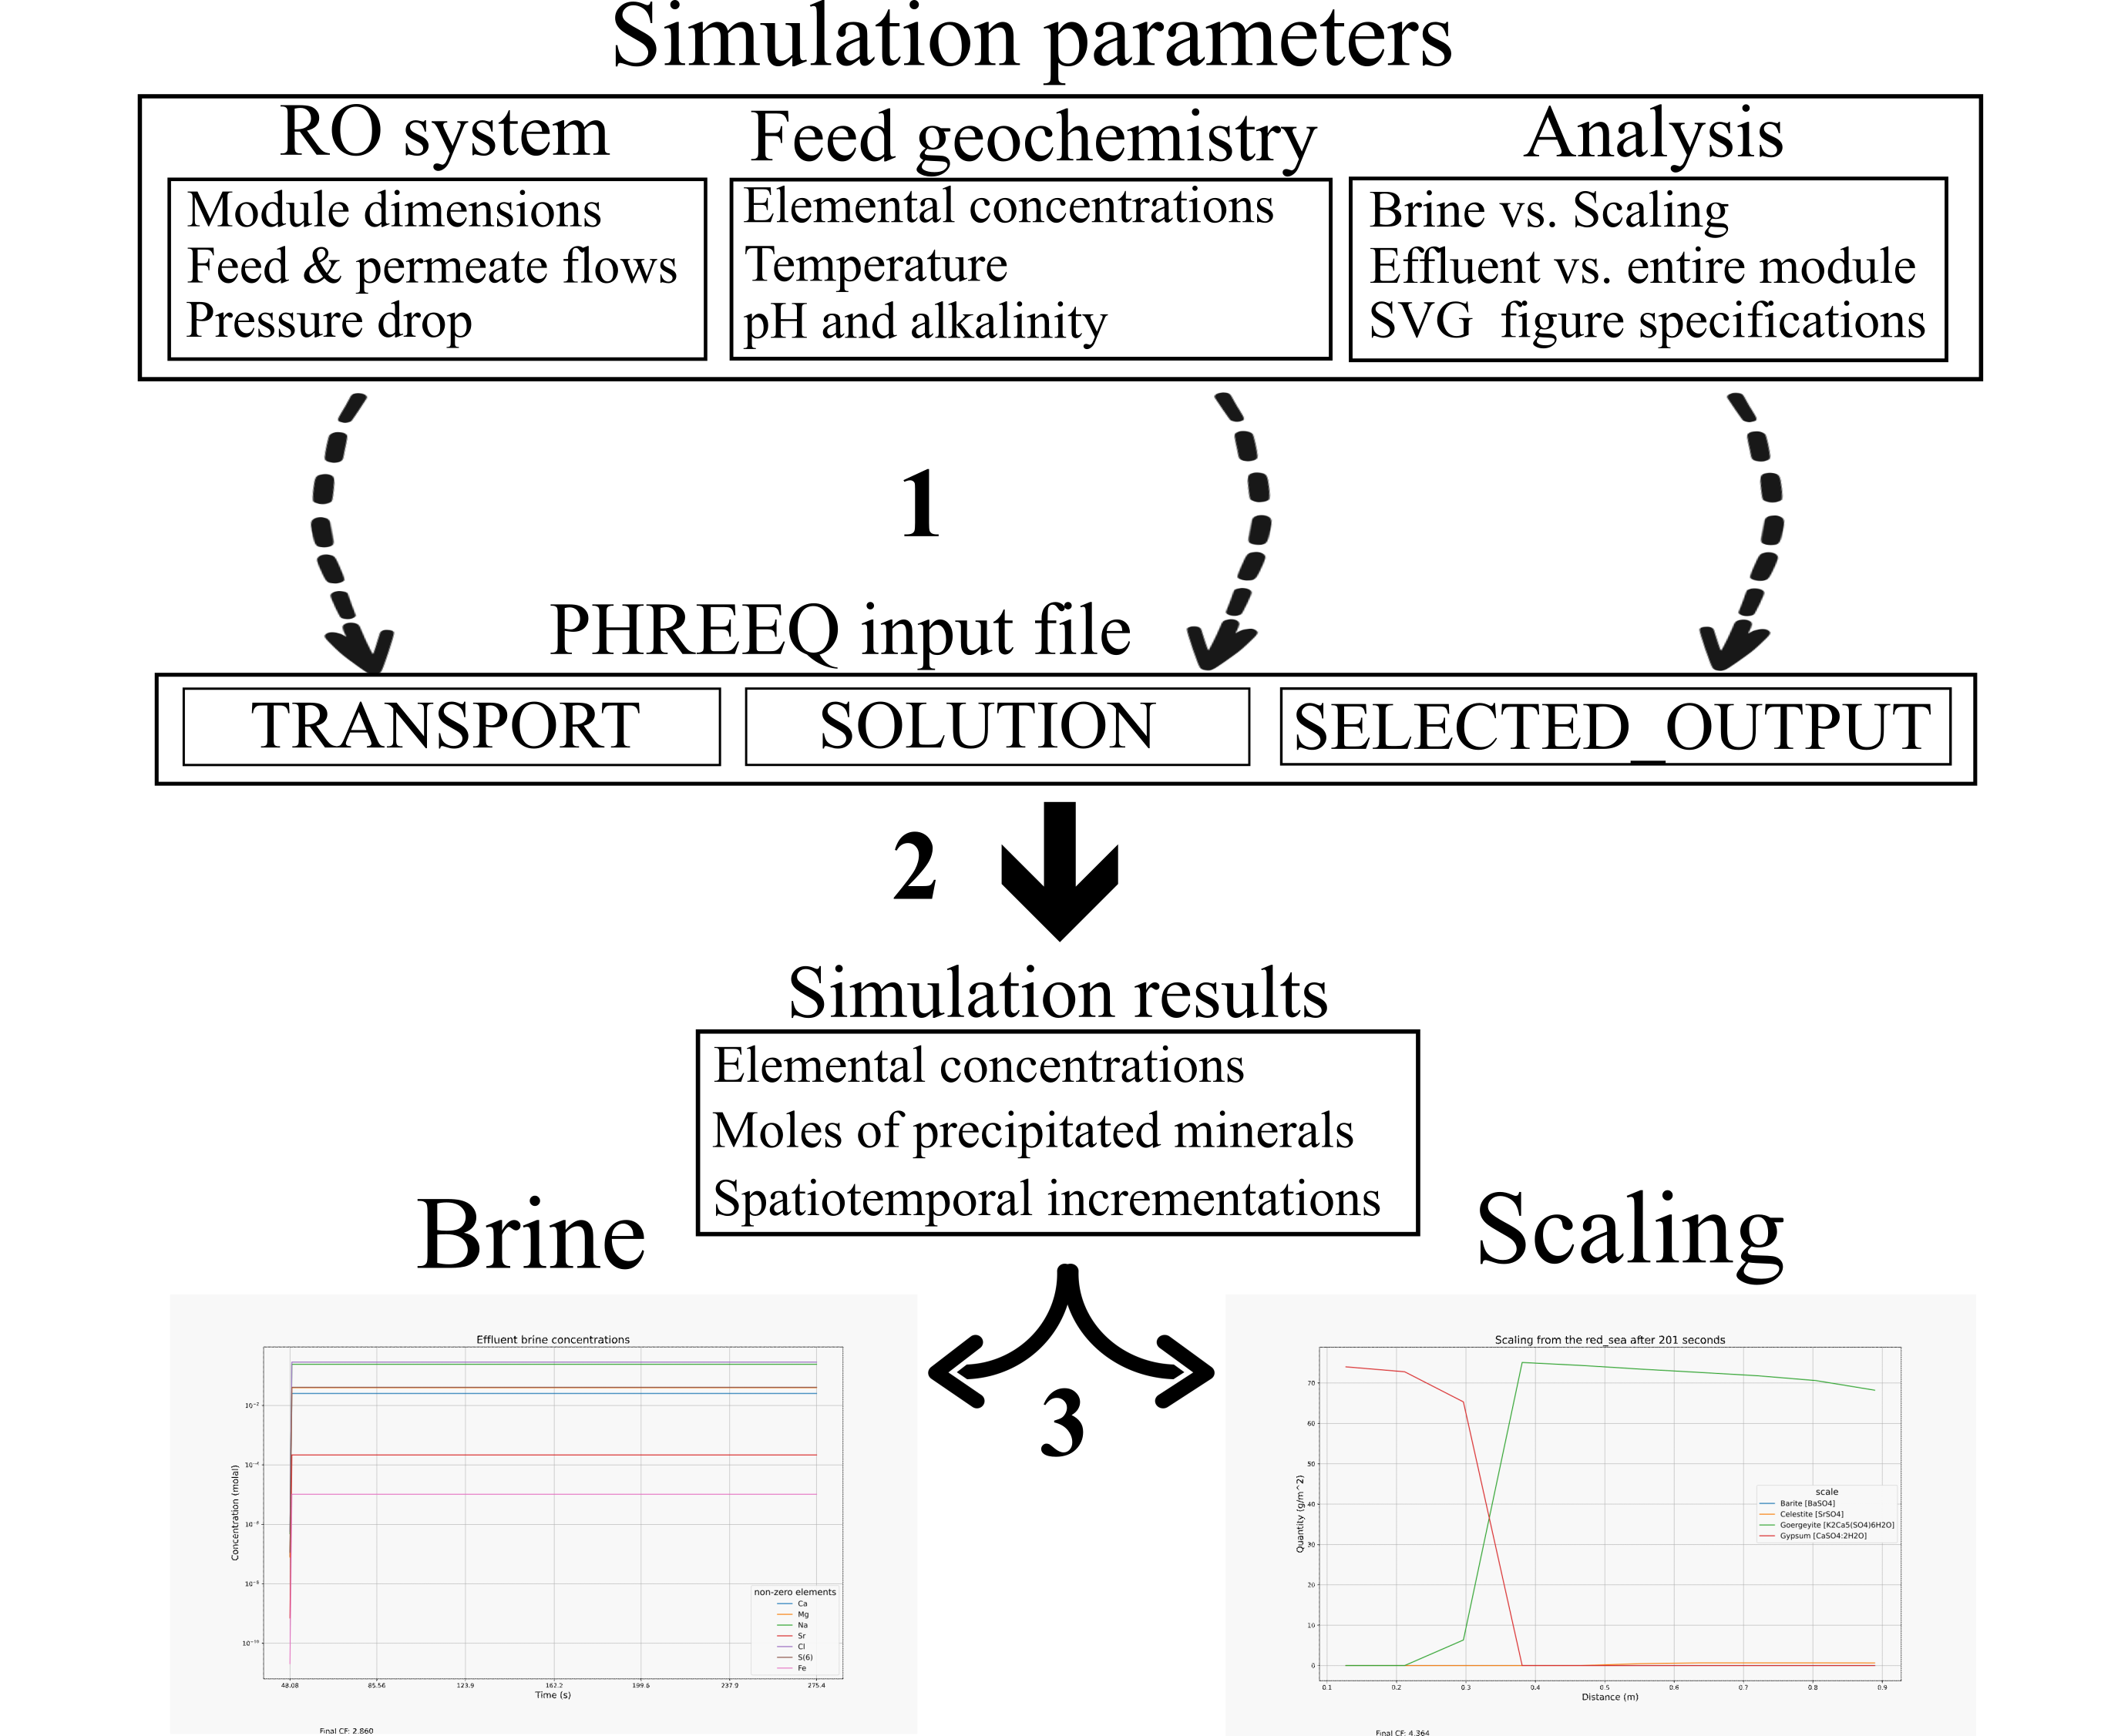
\includegraphics[width = \linewidth]{images/ROSSpy/rosspy_workflow_1.PNG}
    \caption{
        The ROSSpy workflow. Step 1 describes the translation of simulation parameters -- module specifications, feed geochemistry, and simulation analysis -- into PHREEQ code -- the TRANSPORT, SOLUTION, and SELECTED\_OUTPUT blocks, respectively --  via Python logic. Step 2 describes the execution of the PHREEQ input file via either PHREEQpy in the ROSSpy API, or via the PHREEQC batch software in iROSSpy. Step 3 describes processing the predictions of brine concentrations or scaling $\frac{g}{m^2}$ into representative figures and datatables, which are exported with other simulation files.
    }
    \label{workflow}
\end{figure}


\subsection{Numerical}

\subsubsection{Transport}
The transport component of our reactive transport RO model discretizes the membrane-solution interface into $n$ equal fractions (cells) of the total module length $l_{module}$. Feed flow in each timestep is represented by migrating the contents of each cell ($e$) to the next cell ($e+1$), repopulating the first cell ($1$) with new feed solution, and deleting the last cell ($n$) as it conceptually exits the module. The feed velocity $v_{feed}$ is calculated
\begin{equation} \label{feed_velocity}
    v_{feed}=\frac{Q_{max~feed}}{A_{feed}}
\end{equation}
from the maximum feed flowrate $Q_{max~feed}$ and the calculated feed area from \cref{feed_area} of the parameterized RO module. Default module parameters in Table S1, which supplement user-defined module parameters, reflect the DOW FILMTEC BW30-400 RO module as an archetypical RO modules, similar to other models of RO desalination \cite{Li2012OptimalDesalination}. The maximum simulation timestep $\Delta t$ is calculated
\begin{equation} \label{timestep}
    \Delta t=\frac{l_{cell}}{v_{feed}}
\end{equation}
according to the Courant Condition \cite{Gnedin2018EnforcingSchemes} 
\begin{equation} \label{courant_condition}
    C_{max}=1 \ge \frac{v_{feed}*t_{max}}{l_{cell}}
\end{equation}
to ensure that the simulation maintains accuracy over time.


\subsubsection{Reactive geochemistry}
The PHREEQC databases, notwithstanding their pivotal geochemistry, neglect to store the masses of their thousands of minerals, which is essential to determine the predicted $\frac{g}{m^2}$ deposition of scale from a scaling simulation. Contemporary websites and Python modules of PyPI were insufficient to interpret the molecular weight of the complex and heterogeneous inorganic minerals that are encountered in the PHREEQC databases; hence, the ChemW Python package (\url{https://pypi.org/project/ChemW/}) was developed as a rigorous method of calculating the molecular mass from any chemical formula. This provided precisely accurate values that are employed in the scaling predictions, and complements the numerical approaches of our RO module and ROSSpy API per se. 

The permeate flux of the our reactive transport RO model is assumed to be 100\% water, similar to other RO models \cite{Li2012OptimalDesalination}, which is believed to have a negligible significance in geochemical predictions. The calculation of permeate flux primarily involves calculating the moles of feed solution in any examined cell $e$ ($\Phi_e$) and the changes therein from permeate flux over that cell ($\Delta \Phi_{e}$). Permeate flux is generally proportional with transmembrane pressure ($TMP$) and the difference between feed pressure $P$ and osmotic pressure $\pi$ \cite{VanWagner2009EffectPerformance,Schock1987MassModules,Lonsdale1965TransportMembranes}
\begin{equation} \label{pressure_differential}
    \Delta \Phi_{e} ~ \alpha ~ TMP = (P - \pi),
\end{equation} 
however, these pressures are not readily measured or available in literature; thus, we calculate the permeate flux via two comparable methods that are elaborated in the following sections.


\subsubsection{Method 1: Linear permeate flux}
One method assumes that permeate flux is linearly distributed along the RO module according to a calculated flux slope
\begin{equation} \label{flux_slope}
    slope = \frac{(\Delta \Phi_{n}-\Delta \Phi_{1})}{n}
\end{equation}
between cells $1$ and $n$. The permeate fluxes of $\Delta \Phi_{1}$ and $\Delta \Phi_{n}$ are calculated through a system of equations, one of which 
\begin{equation} \label{average_permeate_flux}
     \overbar{\Delta \Phi}_{e} = \frac{\Delta \Phi_{module}}{n} = \frac{\Delta \Phi_{n} + \Delta \Phi_{1}}{2}
\end{equation}
equates the average permeate flux per cell ($\overbar{\Delta \Phi}_{e} = \frac{\Delta \Phi_{module}}{n}$) to the average permeate flux over the module ($\frac{\Delta \Phi_{n} + \Delta \Phi_{1}}{2}$). The second of these equations is the definition of relative pressure head loss \cite{Srivathsan2014ReverseUnsteadiness,Gu2020ModelingNetworks} ($HL ; 0\le HL\le 1$) across the RO module \cite{Fraidenraich2009ReverseExperiment},
\begin{equation} \label{head_loss}
     \Delta \Phi_{n}= \Delta \Phi_{1}*HL,
\end{equation}
as opposed to absolute pressure loss calculations via Darcy's law \cite{Strubbe2018CalibrationFull-Scale}, which causes $\Delta \Phi_{n}<\Delta \Phi_{1}$ per \cref{pressure_differential} as the pressure differential diminishes across the module distance \cite{Li2016Three-dimensionalChannel}. The substitution of \cref{head_loss} into \cref{average_permeate_flux} permits calculating $\Delta \Phi_{1}$ and  $\Delta \Phi_{n}$, the flux slope of \cref{flux_slope}, and subsequently $\Delta \Phi_{e}$
\begin{equation} \label{intermediary_permeate_flux}
    \Delta \Phi_{e} = (slope*e+\Delta \Phi_{1}).
\end{equation}
% Our permeate efficiency parameter ($PE; 0<PE<1$) applies here as means of considering module inefficiencies like preexisting fouling in the RO module that lessen the permeate flux of the system. The $PE$ scalar attenuates the total module permeate flux over the module through reducing \cref{intermediary_permeate_flux}: i.e. $\Delta \Phi_{old~module} = \Delta \Phi_{new~module}*PE$; $PE=0$ leads to $\Delta \Phi_{e}=0 ~\forall~ e$; and $PE=HL=1$ leads to $\overbar{\Delta \Phi}_{e}=\Delta \Phi_{e} ~\forall~ e$.

The equation sequence for this permeate flux method:
\begin{enumerate}
    \item Parameterize the module permeate flux [$\Delta \Phi_{module}$, via the transport() function]
    \item Calculate the permeate flux slope [\cref{flux_slope,average_permeate_flux,head_loss}]
    \item Calculate the permeate flux in each cell [\cref{intermediary_permeate_flux}]
\end{enumerate}


\subsubsection{Method 2: Linear Concentration Factor}
The second method assumes that the feed concentrates linearly, which causes the permeate flux to distribute non-linearly, along the RO module. The concentration factor (CF) \cite{McCaffrey1987TheHalite.,Casas2012SeawaterElectrodialysis,Kartashevsky2015PhosphateEffluents,Yan2017ReverseVelocity} can be calculated with ionic concentrations, solution masses, or permeate moles as the quotient of initial to final  \cite{Casas2012SeawaterElectrodialysis,Yan2017ReverseVelocity}
\begin{equation} \label{cf_definition}
    CF = \frac{initial}{final}
\end{equation}
and represents the multiple to which the effluent is more concentrated than the influent. The CF slope in this permeate flux method is calculated analogously to \cref{flux_slope}:
\begin{equation} \label{average_cf_slope}
    slope_{CF} =\frac{CF_{n}-CF_1}{n}.
\end{equation}
The effluent $CF_{n}$ of the brine solution must be parameterized in ROSSpy, although, it can be easily calculated as the average effluent CF of the feed ions 
\begin{equation} \label{cf_calculation_output}
    CF_{n}=\frac{\sum_{i=1}^j(C_{i,brine})}{\sum_{i=1}^j(C_{i,feed})},
\end{equation}
where $C_{i,brine}$ is the effluent concentration and $C_{i,feed}$ is the influent concentration of ion $i$, for all $j$ ions. Defining CF from \cref{cf_definition} in terms of moles of feed ($\Phi_e$) reveals that the initial $CF=1$ when $e=0$ 
\begin{equation} \label{cf_cell_definition}
    CF_e=\frac{\Phi_0}{\Phi_e}=\frac{\Phi_0}{\Phi_0-\Delta \Phi_{(1,e)}}.
\end{equation}
The $\Phi_e$ moles of feed at the end of cell $e$ from \cref{cf_cell_definition} equates the initial $\Phi_0$ moles of feed minus the sum of permeate flux that occurred between the first cell $1$ and the start of cell $e$ ($\Delta \Phi_{(1,e-1)}=\sum_{j=1}^{e-1}(\Delta \Phi_{j})$) and the permeate flux over cell $e$ ($\Delta \Phi_{e}$):
\begin{equation} \label{moles_removed_to_cell}
    \Delta \Phi_{(1,e)}=\Delta \Phi_{e}+\Delta \Phi_{(1,e-1)}~.
\end{equation}
The initial $\Phi_0$ moles of feed derives from the maximal feed capacity of the simulated module,
\begin{equation} \label{feed_mass}
    \Phi_0=V_{feed}*MW_{H_2O}*\rho_{H_2O},
\end{equation}
where the feed channel volume $V_{feed}$ is calculated from the product of the module length $l_{module}$ and the cross-sectional area of the feed channel $A_{feed}$, where the latter is calculated
\begin{equation} \label{feed_area}
    A_{feed}=(A_{module}-A_{permeate})*\frac{th_{feed}}{th_{unit}},
\end{equation}
from the cross-sectional area of the module $A_{module}$; the cross-sectional area of the permeate tube $A_{permeate}$; the thickness of the feed channel $th_{feed}$; and the thickness of the repeating membrane unit $th_{unit}$ in Figure S1.
The linear expression for $CF_e$ 
\begin{equation} \label{cf_permeate_flux}
    CF_e=(slope_{CF})*e+CF_{0}~,
\end{equation}
is substituted into \cref{cf_cell_definition}, with the slope from \cref{average_cf_slope}, to yield an expression for the permeate flux at the end of the examined cell $e$,
\begin{equation} \label{moles_removal_per_cell} 
    -\Delta \Phi_{(1,e)}=\frac{\Phi_0}{((\frac{CF_{n}-CF_{0}}{n})*e+CF_{0})}-\Phi_0~,
\end{equation}
which can be substituted into \cref{moles_removed_to_cell} with the sum of previous permeate fluxes ($\Delta \Phi_{(1,e-1)}$) to yield the permeate flux for any examined cell $e$ ($\Delta \Phi_{e}$). Note that $\Delta \Phi_{(1,e-1)}=0$ when $e=1$, since there are no previous cells. 

The equation sequence for this permeate flux method:
\begin{enumerate}
    \item Parameterize the effluent CF [via the reactions() function]
    \item Calculate the feed capacity of the module [\cref{feed_mass,feed_area}]
    \item Calculate the CF slope [\cref{average_cf_slope}]
    \item Calculate the permeate flux in each cell [\cref{cf_cell_definition,moles_removed_to_cell,cf_permeate_flux,moles_removal_per_cell}]
\end{enumerate}


\subsubsection{Comparison of permeate flux methods}
Scaling predictions from the two permeate flux methods -- linear permeate flux and linear CF -- are juxtaposed in Figure \ref{permeate_approach}. The most significant difference is observed at the mid-point of the simulated module ($0.47 m$), where the linear CF simulation predicts $0.99 \frac{gram}{m^2}$ of Gypsum scale while the linear permeate flux simulation predicts $0.0196 \frac{gram}{m^2}$ of Gypsum scale. These differences, however, are ultimately averaged-out, where the predicted quantity of scale over the entire module is identical between these two methods to 3 significant digits ($38.7 \frac{gram}{m^2}$). The permeate flux method is therefore believed to subtly affect only the distribution, and not the total quantity, of scale within a module. 

\begin{figure}[h]
    \centering
    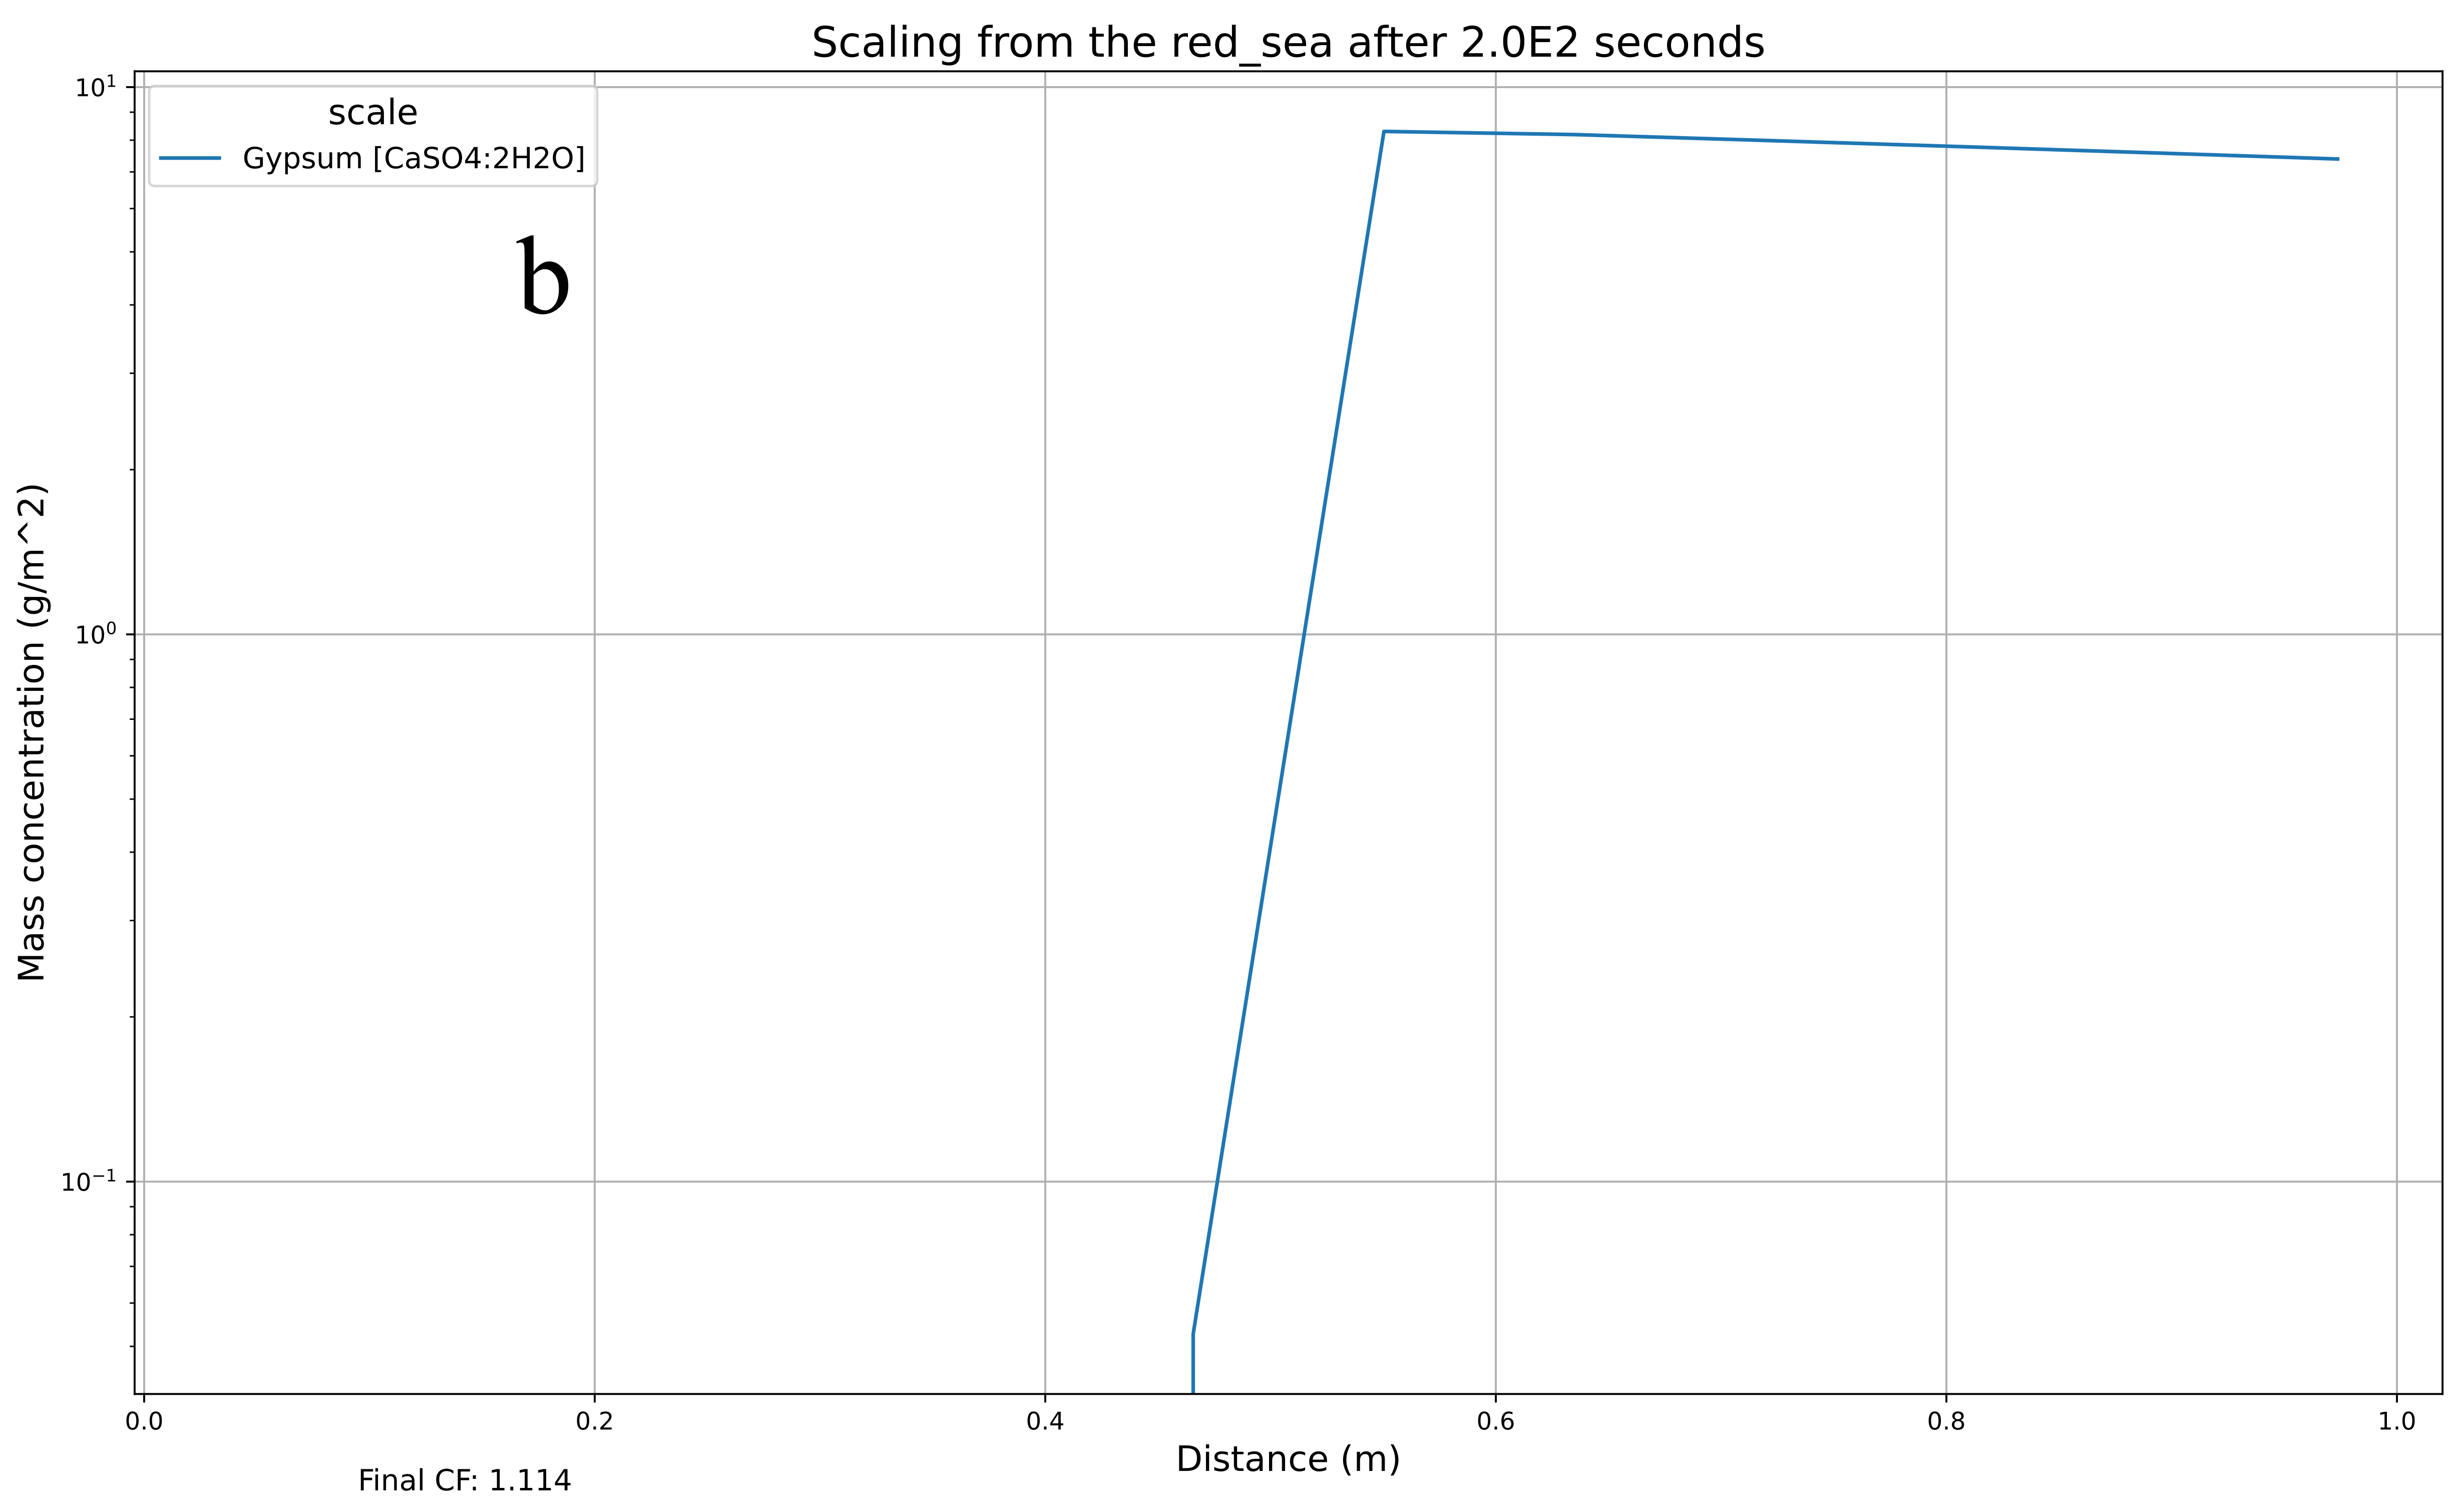
\includegraphics[width=\linewidth]{images/ROSSpy/sensitivity_analyses/permeate_approach/linear_permeate.png} \\ \midrule
    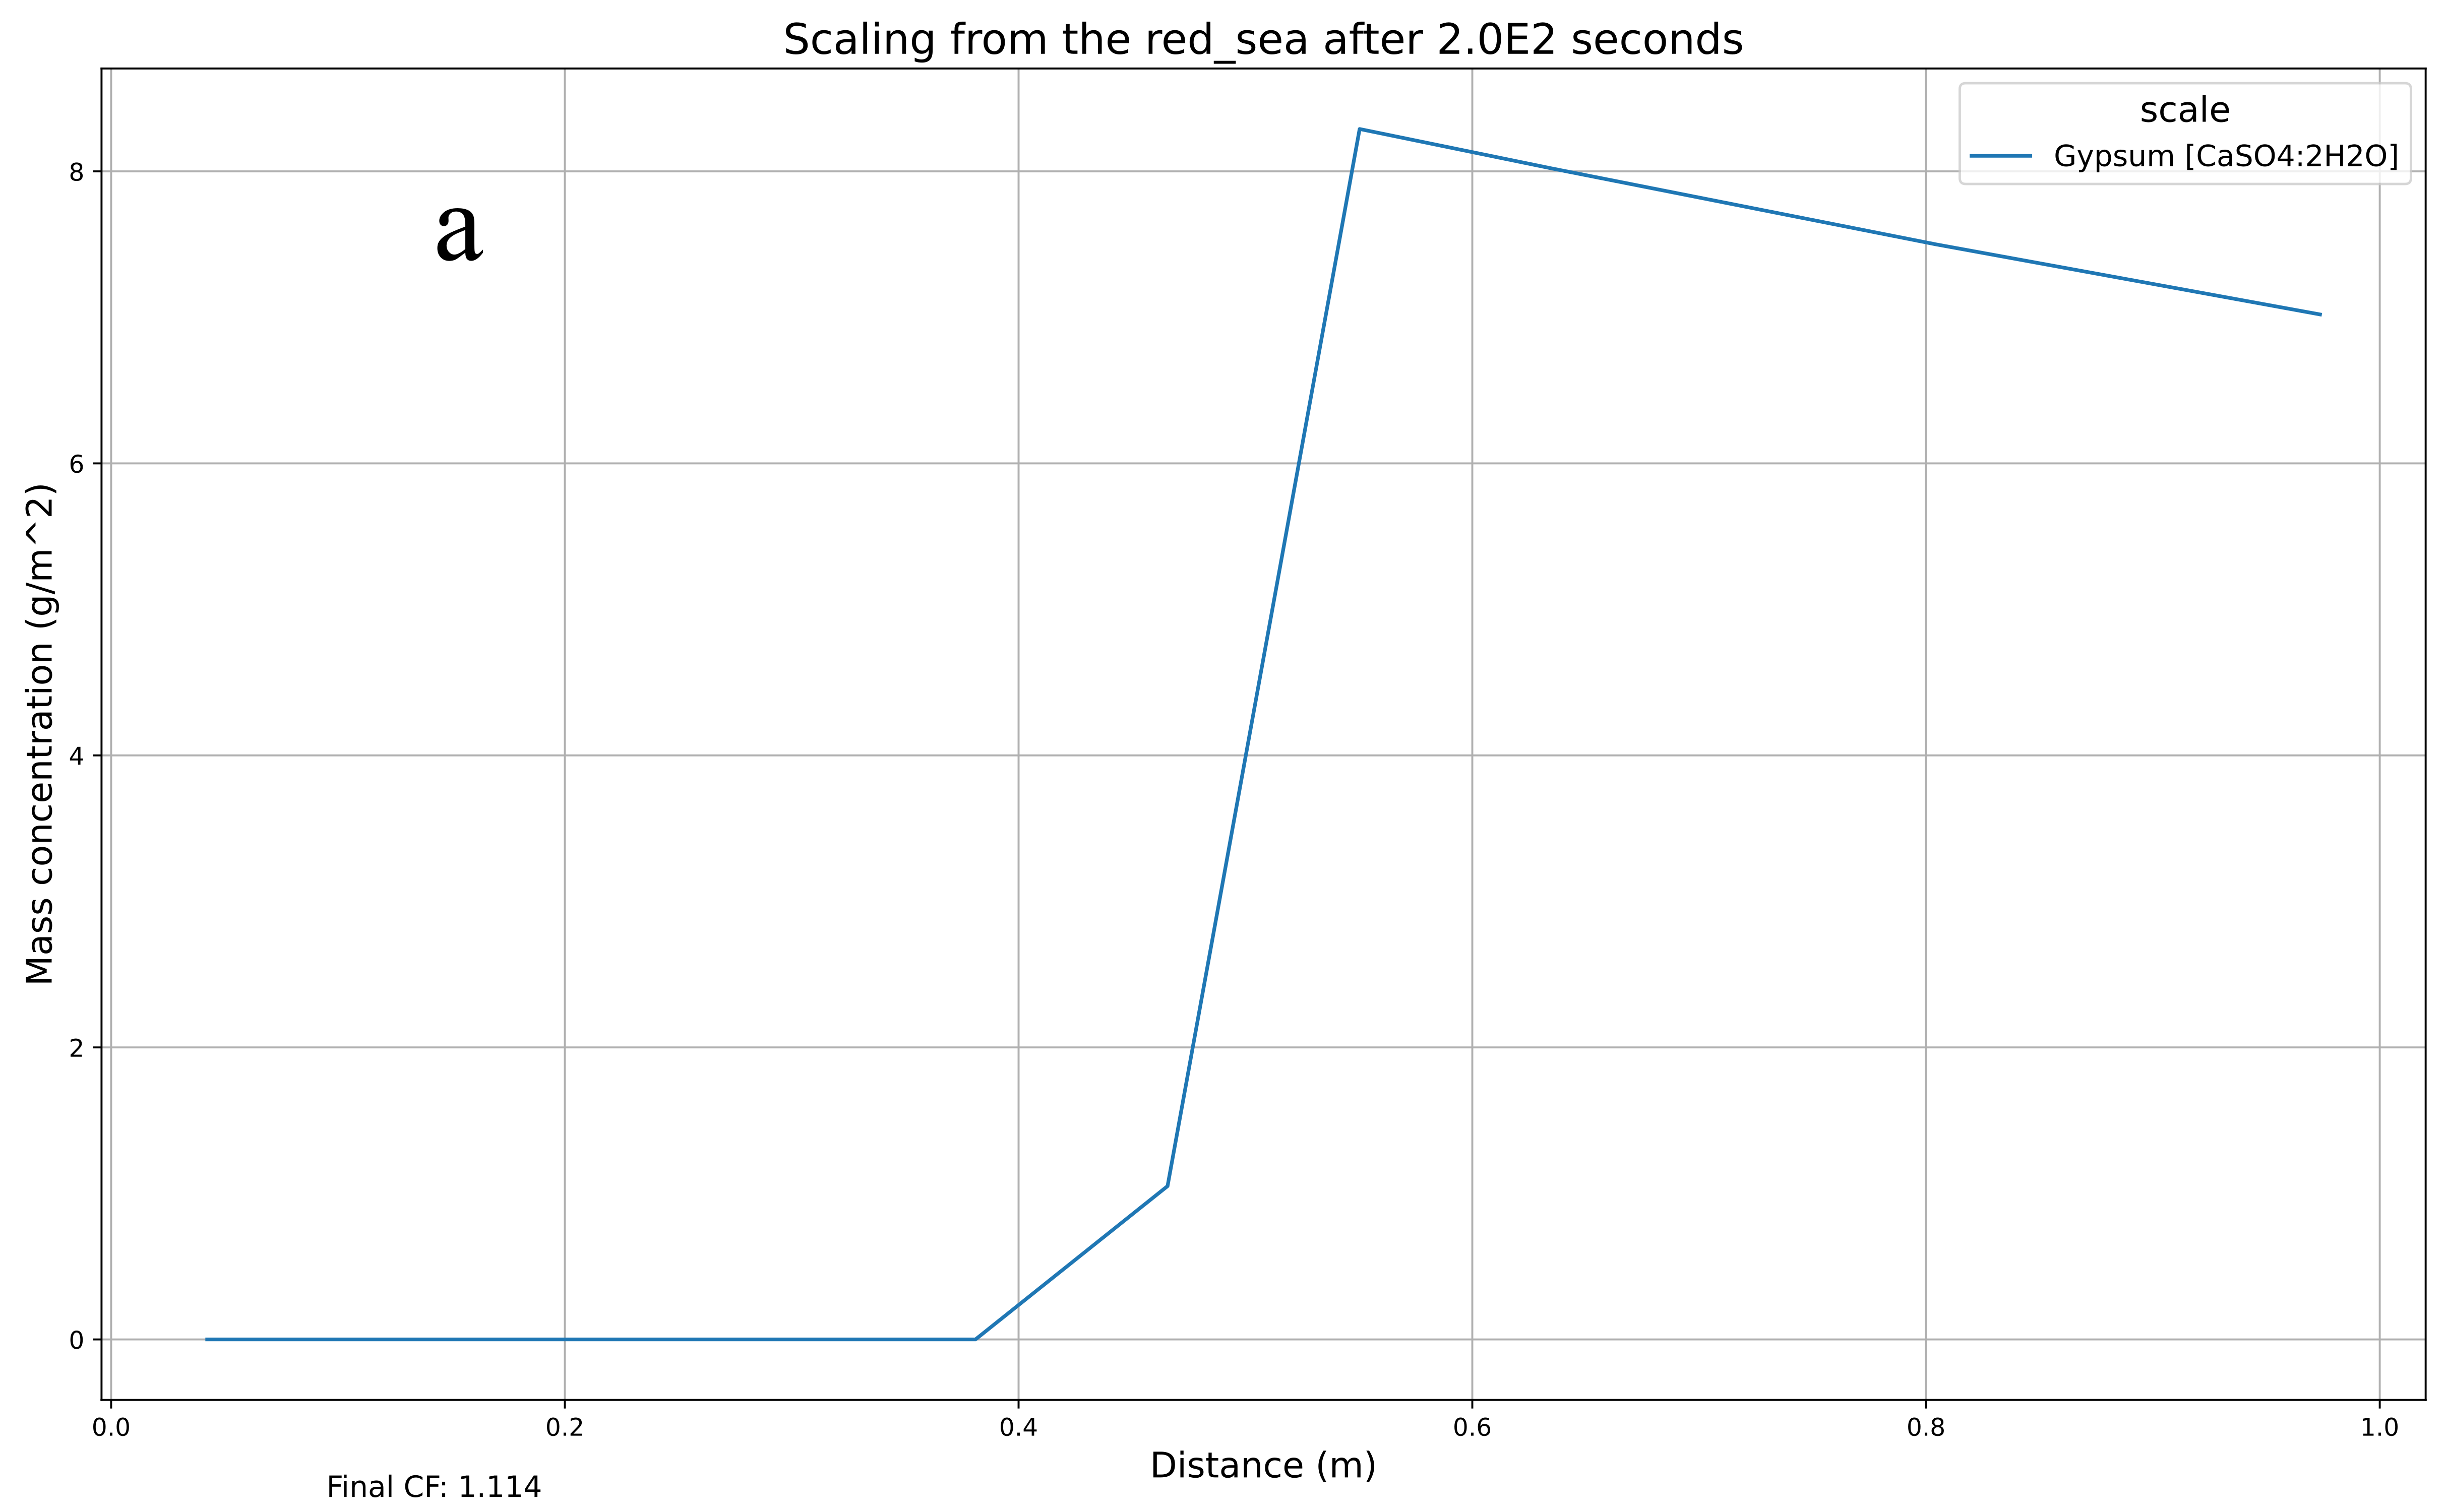
\includegraphics[width=\linewidth]{images/ROSSpy/sensitivity_analyses/permeate_approach/linear_cf.png} 
    \caption{
        Predicted scaling, of the Red Sea at $CF_{effluent}=1.114$, via the a) linear permeate flux and the b) linear CF calculation methods. 
    }
    \label{permeate_approach}
\end{figure}


\subsection{Software}
ROSSpy is the embodiment of our one-dimensional RO model, and post-processing of simulation results. The software conducts a sequence of tasks: 1) translates user inputs into a PHREEQ input file; 2) executes the PHREEQ simulation file; and 3) processes the simulation results, either over the entire module distance at the final time or over all timesteps at the final module distance, into figures and data tables; and 4) exports all of the simulation content -- e.g. PHREEQ input file, SVGs figures, and CSVs of parameters, variables, data, and brine predictions -- into the specified folder and directory. The API documentation for ROSSpy on our PyPI and GitHub pages elaborates the operations and syntax of ROSSpy.


\subsubsection{Water bodies}
Users of ROSSpy are encouraged to simulate their own feed water sources, which can be defined in an argument dictionary or as a JSON file of feed parameters. A default set of feed waters are provided in \verb|rosspy\water_bodies|, which were assembled from experimental geochemical literature. We propose experimental data for numerous potential feed water sources in Table S2 that a user can adapt into feed water parameters; although, anthropogenic pollution \cite{Chen2008SourcesSea} and seasonality \cite{Sarthou2001SeasonalSea} are known to significantly alter the geochemistry of water bodies, so direct analysis of the simulated feed water is preferable to using potentially out-dated experimental measurements. 


\section{Verification}
The following subsections demonstrate the accuracy of ROSSpy predictions through various use-cases. The Python Notebooks and simulation folders for each subsection are shared in \verb|ROSSpy\examples| of our GitHub repository.


\subsection{CF and Brine formation}
The predicted effluent brine concentrations and effluent CF from our model were verified through comparison with the following three experimental papers, where the reported brine concentrations were compared with the ROSSpy predictions after the the feed geochemistry and RO module specifications were parameterized into ROSSpy. 

\paragraph{Zaman et al.\cite{Zaman2015DownstreamCompounds}}
This study  examines RO brine, from a full-scale water treatment facility in Australia, to understand which scalants are likely to develop from the feed source. The ROSSPy predictions in Figure \ref{bar_graphs}a were $<6\%-error$ for all but one of the feed ions.

\paragraph{Ahmed et al.\cite{Ahmed2001BrineEmirates}}
This study  evaluates the RO brine from 10 small desalination plants in Oman and 8 plants in the United Arab Emirates (UAE) for the purpose of understanding ideal brine disposal methods for each brine source. We selected the UAE Qidfa I desalination plant from these 18 plants to evaluate, since it is reported more comprehensively than the other plants. The ROSSPy predictions in Figure \ref{bar_graphs}b were $<10\%-error$ for all but one of the feed ions.

\paragraph{Hajbi et al.\cite{Hajbi2010ReuseBrine}}
This study  evaluates the recovery of commodity salts from RO brine at a plant in Tunisia. The authors detail specifications of line D -- a polyamide filtration membrane -- in the plant system, in addition to the feed geochemistry, that were parameterized into ROSSpy.  The ROSSPy predictions in Figure \ref{bar_graphs}c were less accurate than the aforementioned two studies, with two ions exceeding $25\%$, which may extend from relatively fewer feed ions being defined, which creates an incomplete geochemical approximation of the feed water. This is corroborated by the accuracy of the calculated CF with the reported CF: i.e. the calculations are accurate yet the data may be incomplete.

\paragraph{CF verification}
The effluent CF from each of the aforementioned papers, in the far-right columns of each sub-figure in Figure \ref{bar_graphs}, which was calculated via water mass change in \cref{cf_definition}, deviates by $[0.78, 2.3]-\%$. This accuracy affirms the permeate flux calculation methods, and is well within the margin of error that is attributed to feed parameters, as represented by the $\%-error$ of the ionic concentrations.

\begin{figure}[h]
    \centering
    \begin{tabular}{c|c}
        \multicolumn{2}{c}{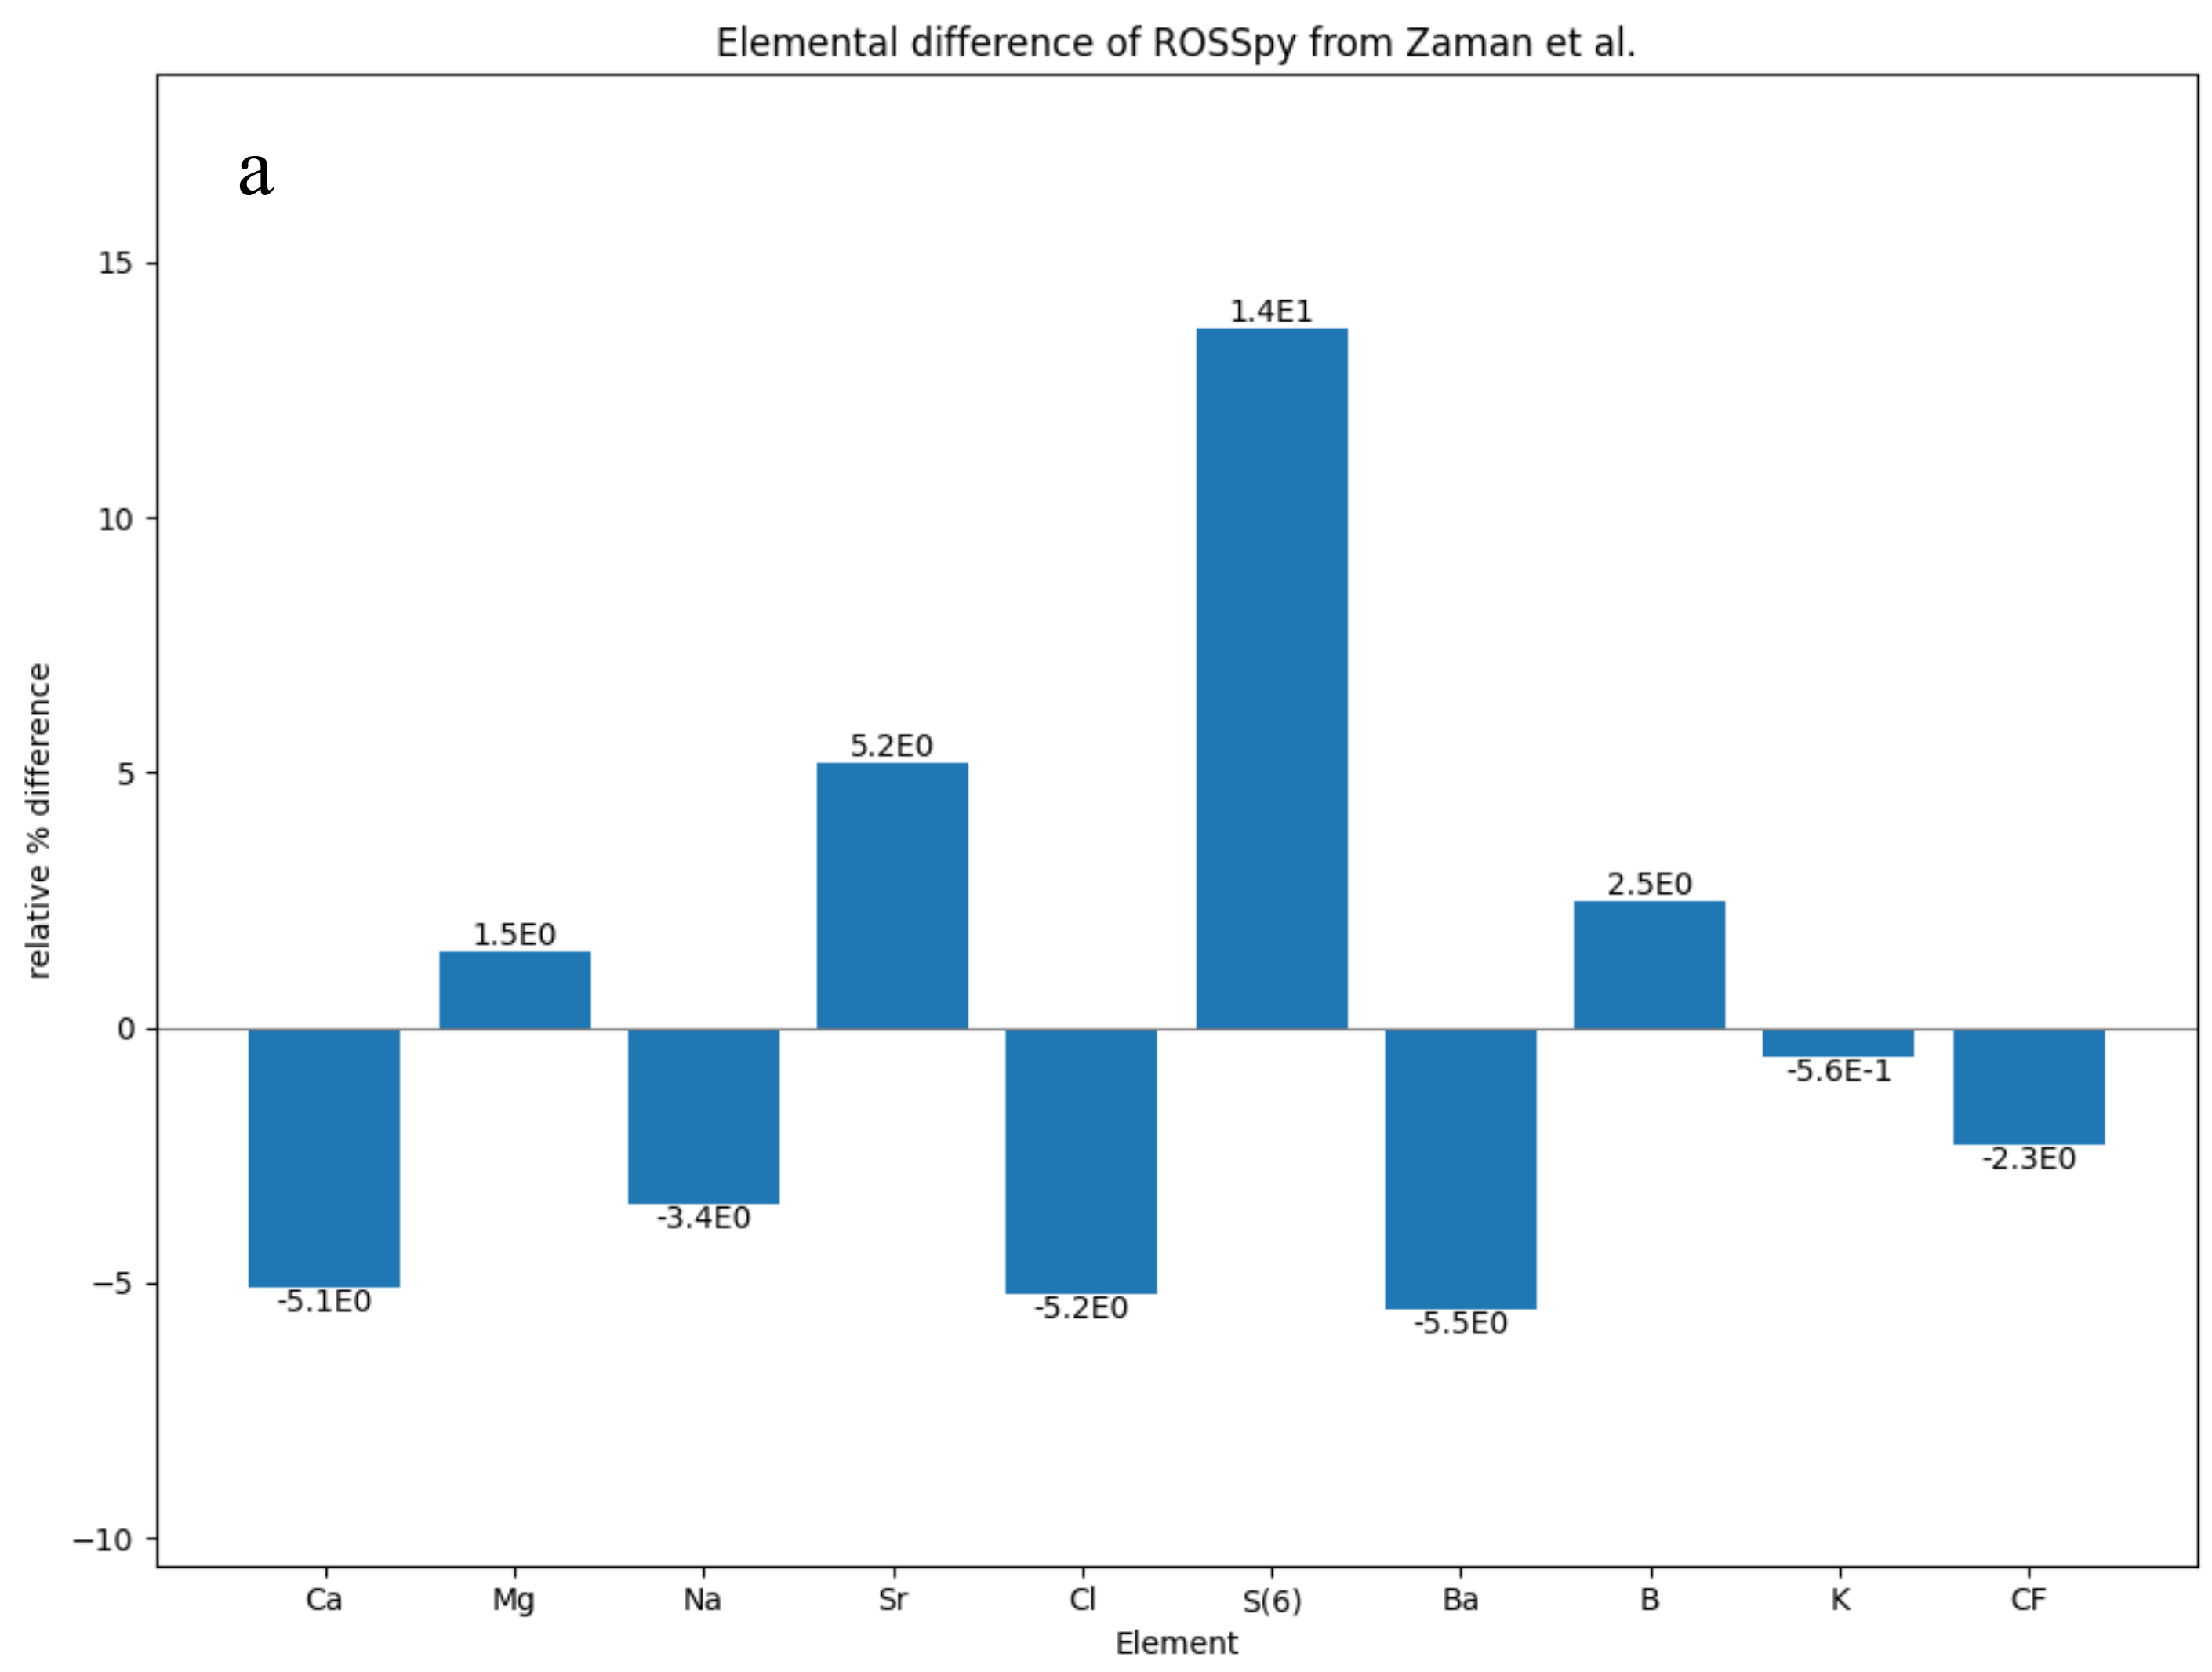
\includegraphics[width=\linewidth]{images/ROSSpy/case_studies/Zaman_comparison.png}} \\ \midrule
        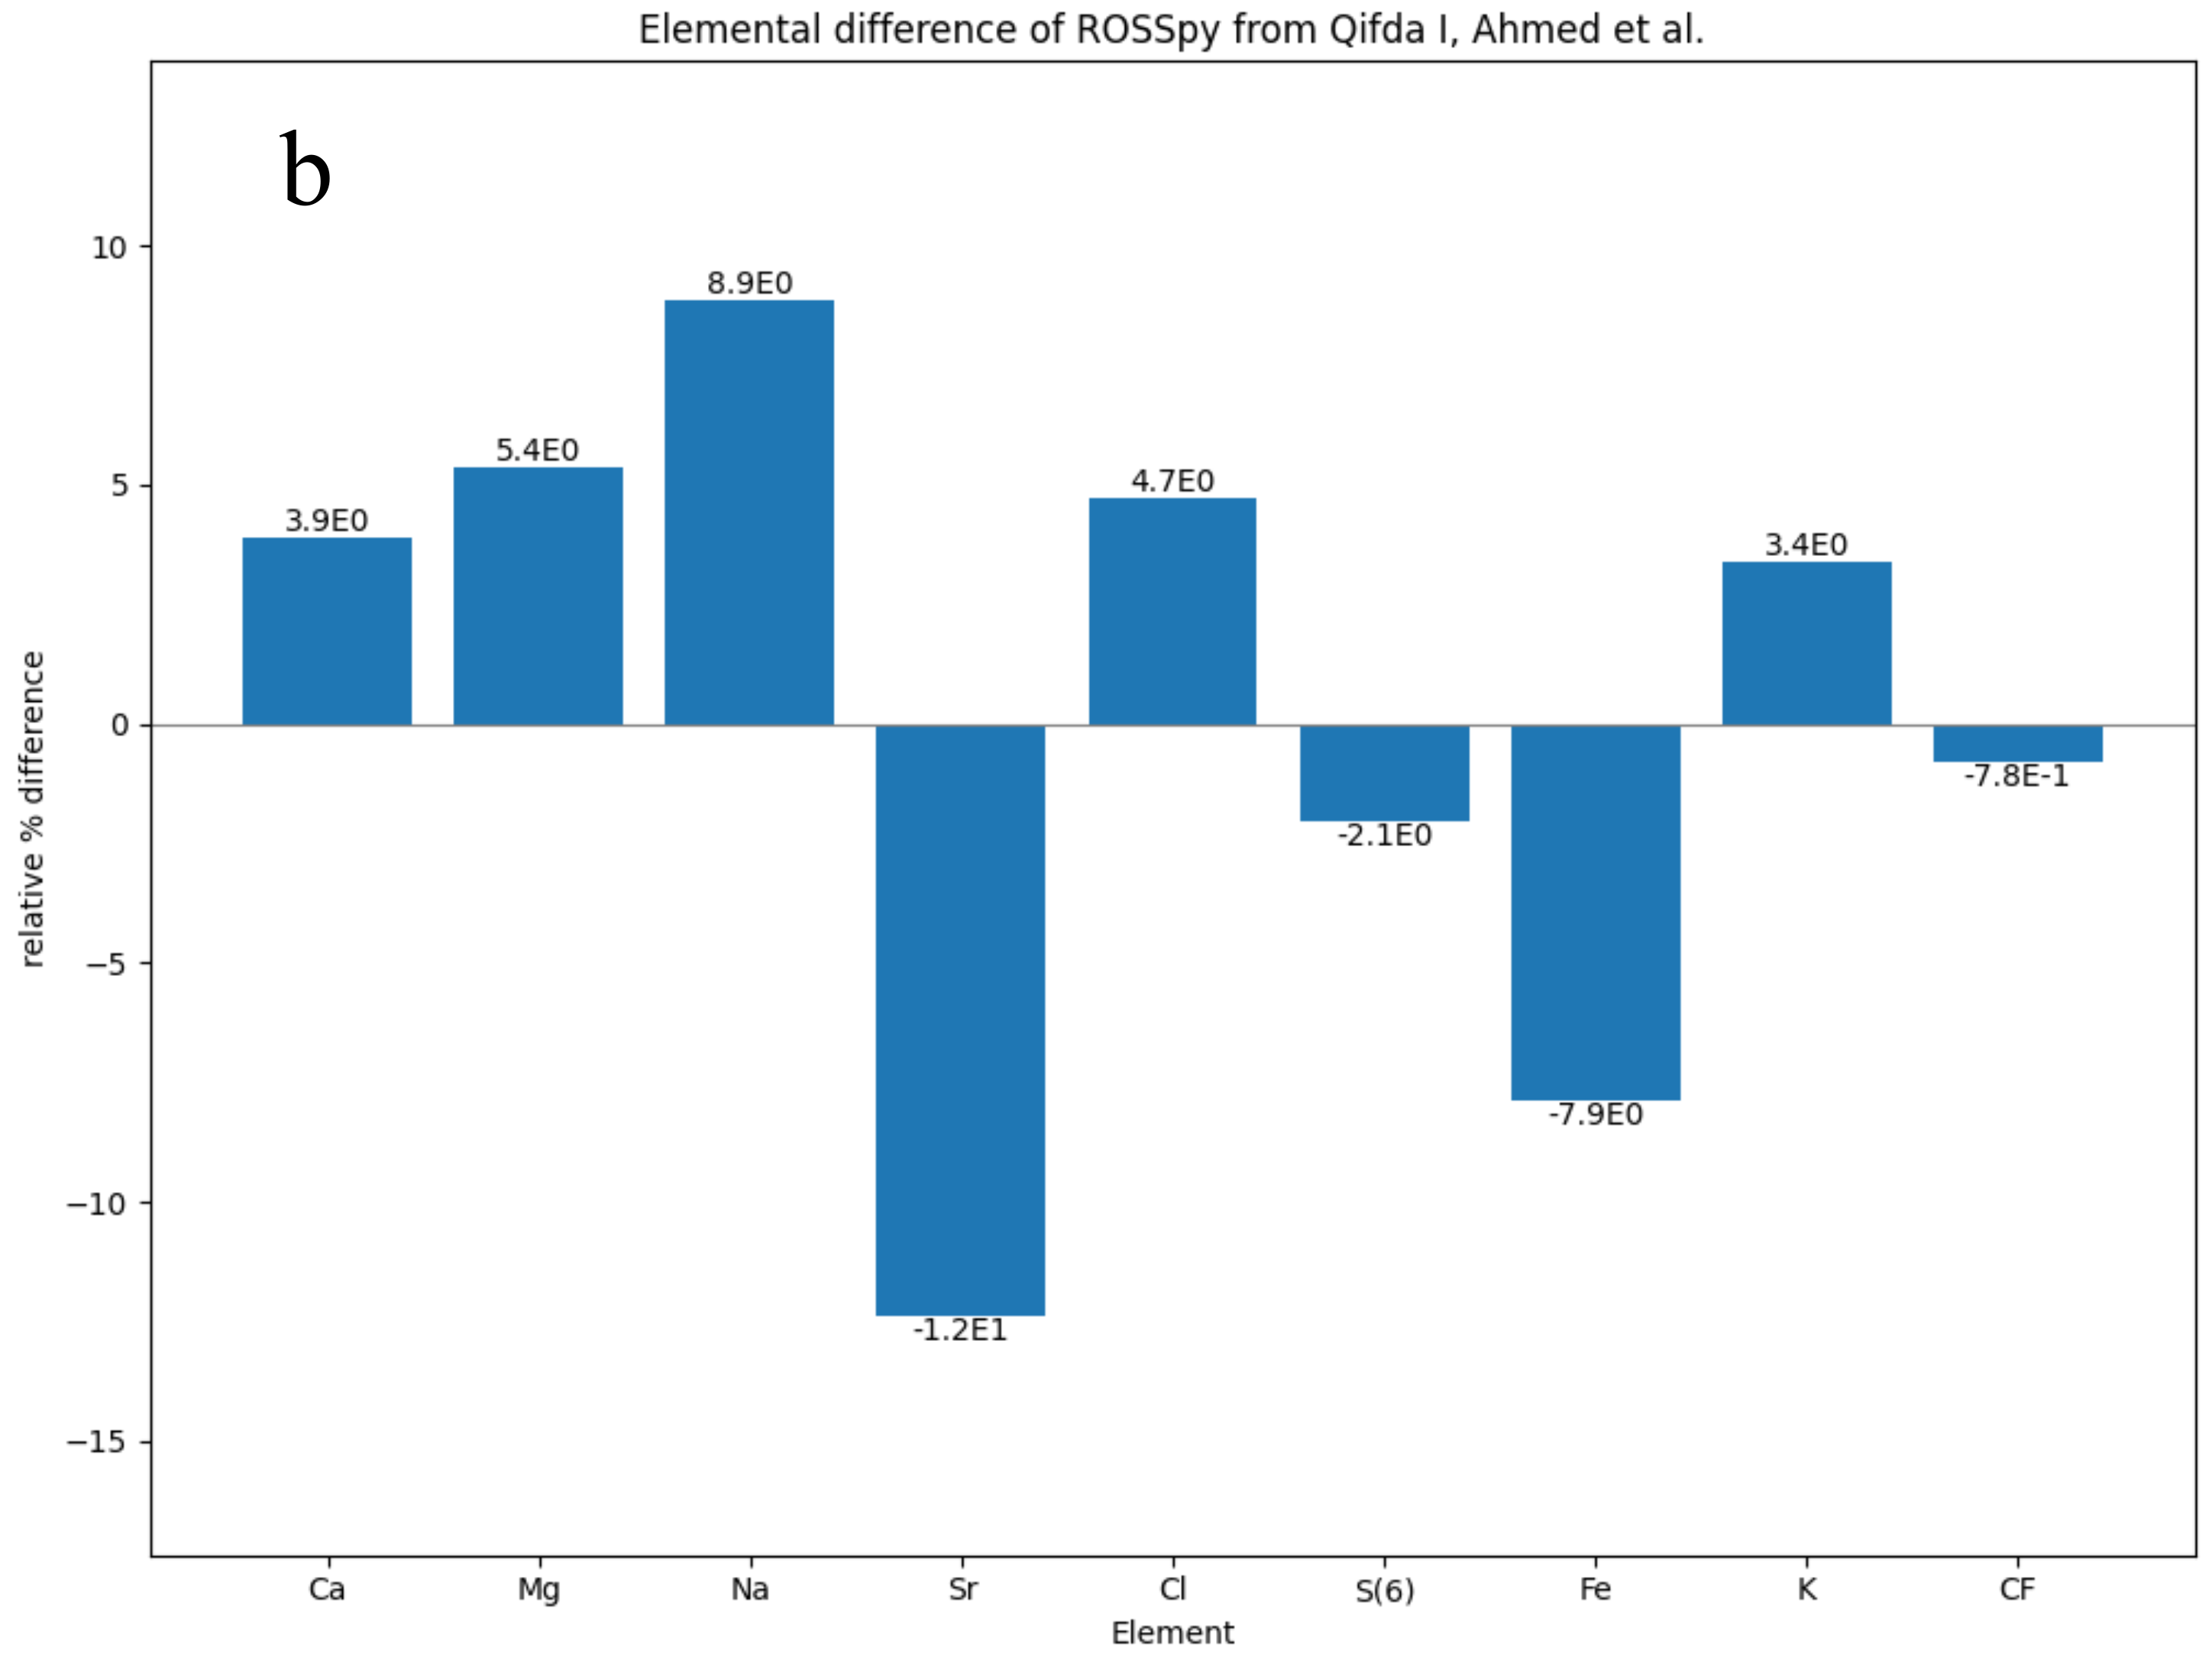
\includegraphics[width=0.49\linewidth]{images/ROSSpy/case_studies/Ahmed_comparison.png} & 
        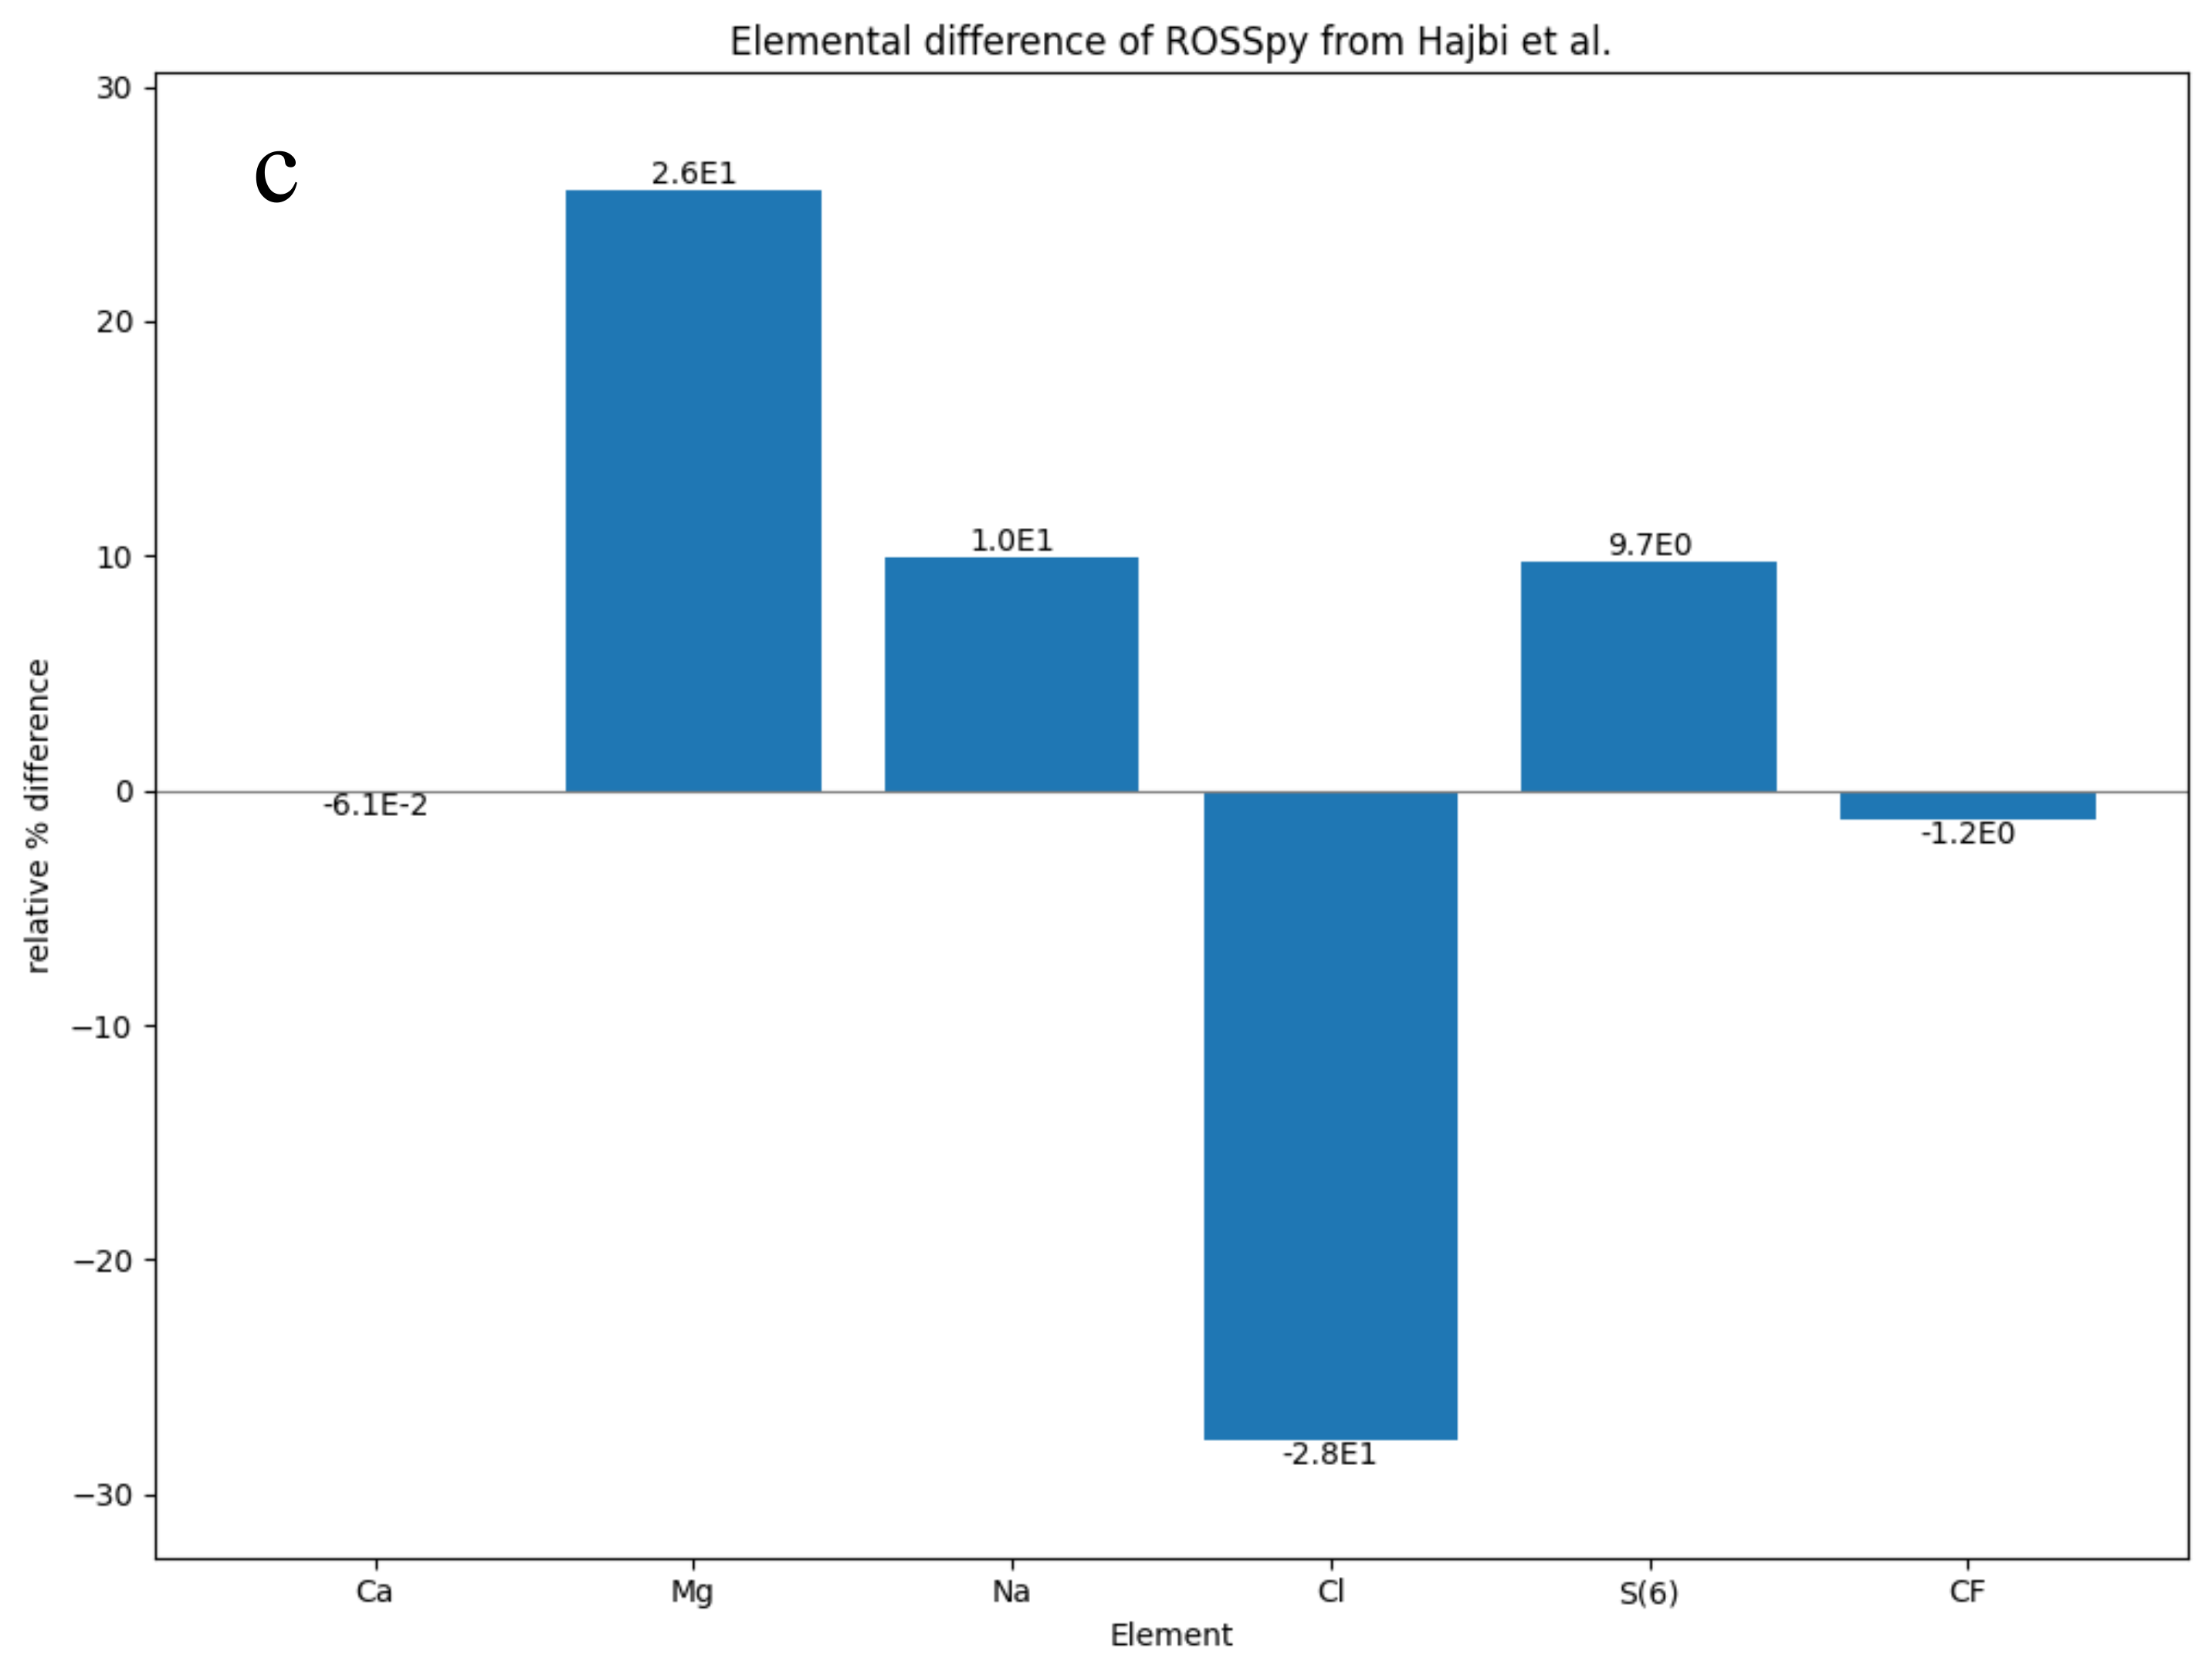
\includegraphics[width=0.49\linewidth]{images/ROSSpy/case_studies/Hajbi_comparison.png} \\ \bottomrule
    \end{tabular}
    \caption{
        The \%-error between the predicted effluent brine concentrations from ROSSpy and the experimental brine measurements from RO plants. Panels a-c) correspond with the Zaman et al. \cite{Zaman2015DownstreamCompounds}, Ahmed et al. \cite{Ahmed2001BrineEmirates}, and Hajbi et al. \cite{Hajbi2010ReuseBrine} studies, respectively, and each possess different y-axis scales to best resolve the bars in each graph. 
    }
    \label{bar_graphs}
\end{figure}


\subsection{Scaling}
The scaling predictions were verified quantitatively and qualitatively, from theoretical calculations and experimental literature, respectively. Experimental literature was not discovered that quantified scaling while also articulating the feed geochemistry that produced the scale. 

\subsubsection{Quantitative}
The precipitation equilibria of PHREEQC were quantitatively verified through an ICE table for a simple case of Gypsum precipitation. The predicted $0.01961$ moles of Gypsum precipitation from PHREEQ, in Table \ref{gypsum_ice_table}a, is 7\% greater than the $0.01859$ moles that is expected based upon the stoichiometry of the equilibrium reaction. This deviation is attributed to the printed concentrations from PHREEQC, which comprise Table \ref{gypsum_ice_table}a, only embodying advection and not embodying the diffusion that also influences RO reactive transport. The same $+7\%$-error was observed between $0.194$ moles predicted from simulating desalination of the Red Sea (solved in eq. S2) versus $0.181$ moles that are expected from a simple system of $Ca^{2+}$ and $SO_4^{2-}$ ions in Table \ref{gypsum_ice_table}b (solved in eq. S1). This deviation is attributed to ionic interactions of the Red Sea feed that are not considered in the simplified system of only $Ca^{2+}$ and $SO_4^{2-}$. These subtle 7\% deviations, notwithstanding their complexities beyond the scope of ICE tables, are relatively minor in the context of other sources of error, e.g. feed measurements, and still provide close quantitative estimates of scaling.

\begin{table}
    \centering
    \begin{tabular}{c|ccccc}
      \toprule
      \textbf{a} & $Ca^{2+}$ & $+$ & $SO_4^{2-}$ & $\leftrightharpoons$ & $CaSO_4$ \\
      \midrule
      I & $0.3545$ && $1.816$ && $0$ \\
      C & $-0.01859$ && $-0.01859$ && $+0.01961$ \\
      F & $0.3360$ && $1.797$ && $0.01961$ \\
      \bottomrule
      \\
      \toprule
      \textbf{b} & $Ca^{2+}$ & $+$ & $SO_4^{2-}$ & $\leftrightharpoons$ & $CaSO_4$ \\
      \midrule
      I & $0.003913$ && $0.00633$ && $0$ \\
      C & $-x$ && $-x$ && $+x$ \\
      F & $0.003913-x$ && $0.00633-x$ && $x$ \\
      \bottomrule
    \end{tabular}
    \caption{
        Gypsum precipitation according to the ICE (Initial, Change, Equilibrium) model, except that "Equilibrium" (E) is replaced with "Final" (F) since the system never completely reaches equilibrium before the solution leaves the simulated module. The bottom ICE table estimated Gypsum precipitation after desalination -- based upon the $K_{sp}$ of Gypsum and the activity coefficients of the feed solution from iPHREEQC -- in eq. S1. 
      }
    \label{gypsum_ice_table}
\end{table}

\subsubsection{Qualitative}
The scaling predictions from ROSSpy were qualitatively verified through comparison with the following three experimental studies. 

\paragraph{Karabelas et al., 2020 \cite{Karabelas2020ScalingTools}}
This study reviews the state-of-the-art for software that predicts RO scaling, which inspired the development and features of ROSSpy, and provides in the supporting information details of feed geochemistry and module specifications for an RO desalination plant. The scale predictions in Figure \ref{qualitative_scaling}a from these parameters exactly match the reported scale observations ("Calcite but not Gypsum" and a "few other salts, such as Barite and Dolomite, could also deposit at downstream...") in numerous ways: 1) Calcite was the primary scalant; 2) Gypsum was not a predicted scalant; 3) a few other salts precipitated with lesser quantity, including Dolomite and Barite; and 4) the minor salts, primarily Dolomite, precipitated more in the downstream portion of the module.  

\paragraph{Karabelas et al., 2014 \cite{Karabelas2014IncipientChannels}}
This study elucidates the mechanisms of incipient scaling from RO desalination -- with Gypsum as the archetypal scalant \cite{Lyster2009CoupledModule,Radu2014ASystems}. The ionic concentrations of from the trial ID 28SC in the paper were parameterized into ROSSpy, and the only predicted scalant was Gypsum in Figure \ref{qualitative_scaling}b, identically to the study.  

\paragraph{Lee et al., 2009 \cite{Lee2009MembraneWastewater}}
The study  evaluates the use of a membrane bioreactor -- which is a hollow-fiber membrane module design that is mechanistically similar to RO and thus can be represented by the same reactive transport model as RO -- to treat wastewater. The wastewater feed geochemistry was parameterized into ROSSpy, and only predicted scalant was Calcite in Figure \ref{qualitative_scaling}c, identically to the study.

\begin{figure}
    \begin{tabular}{c|c}
        \multicolumn{2}{c}{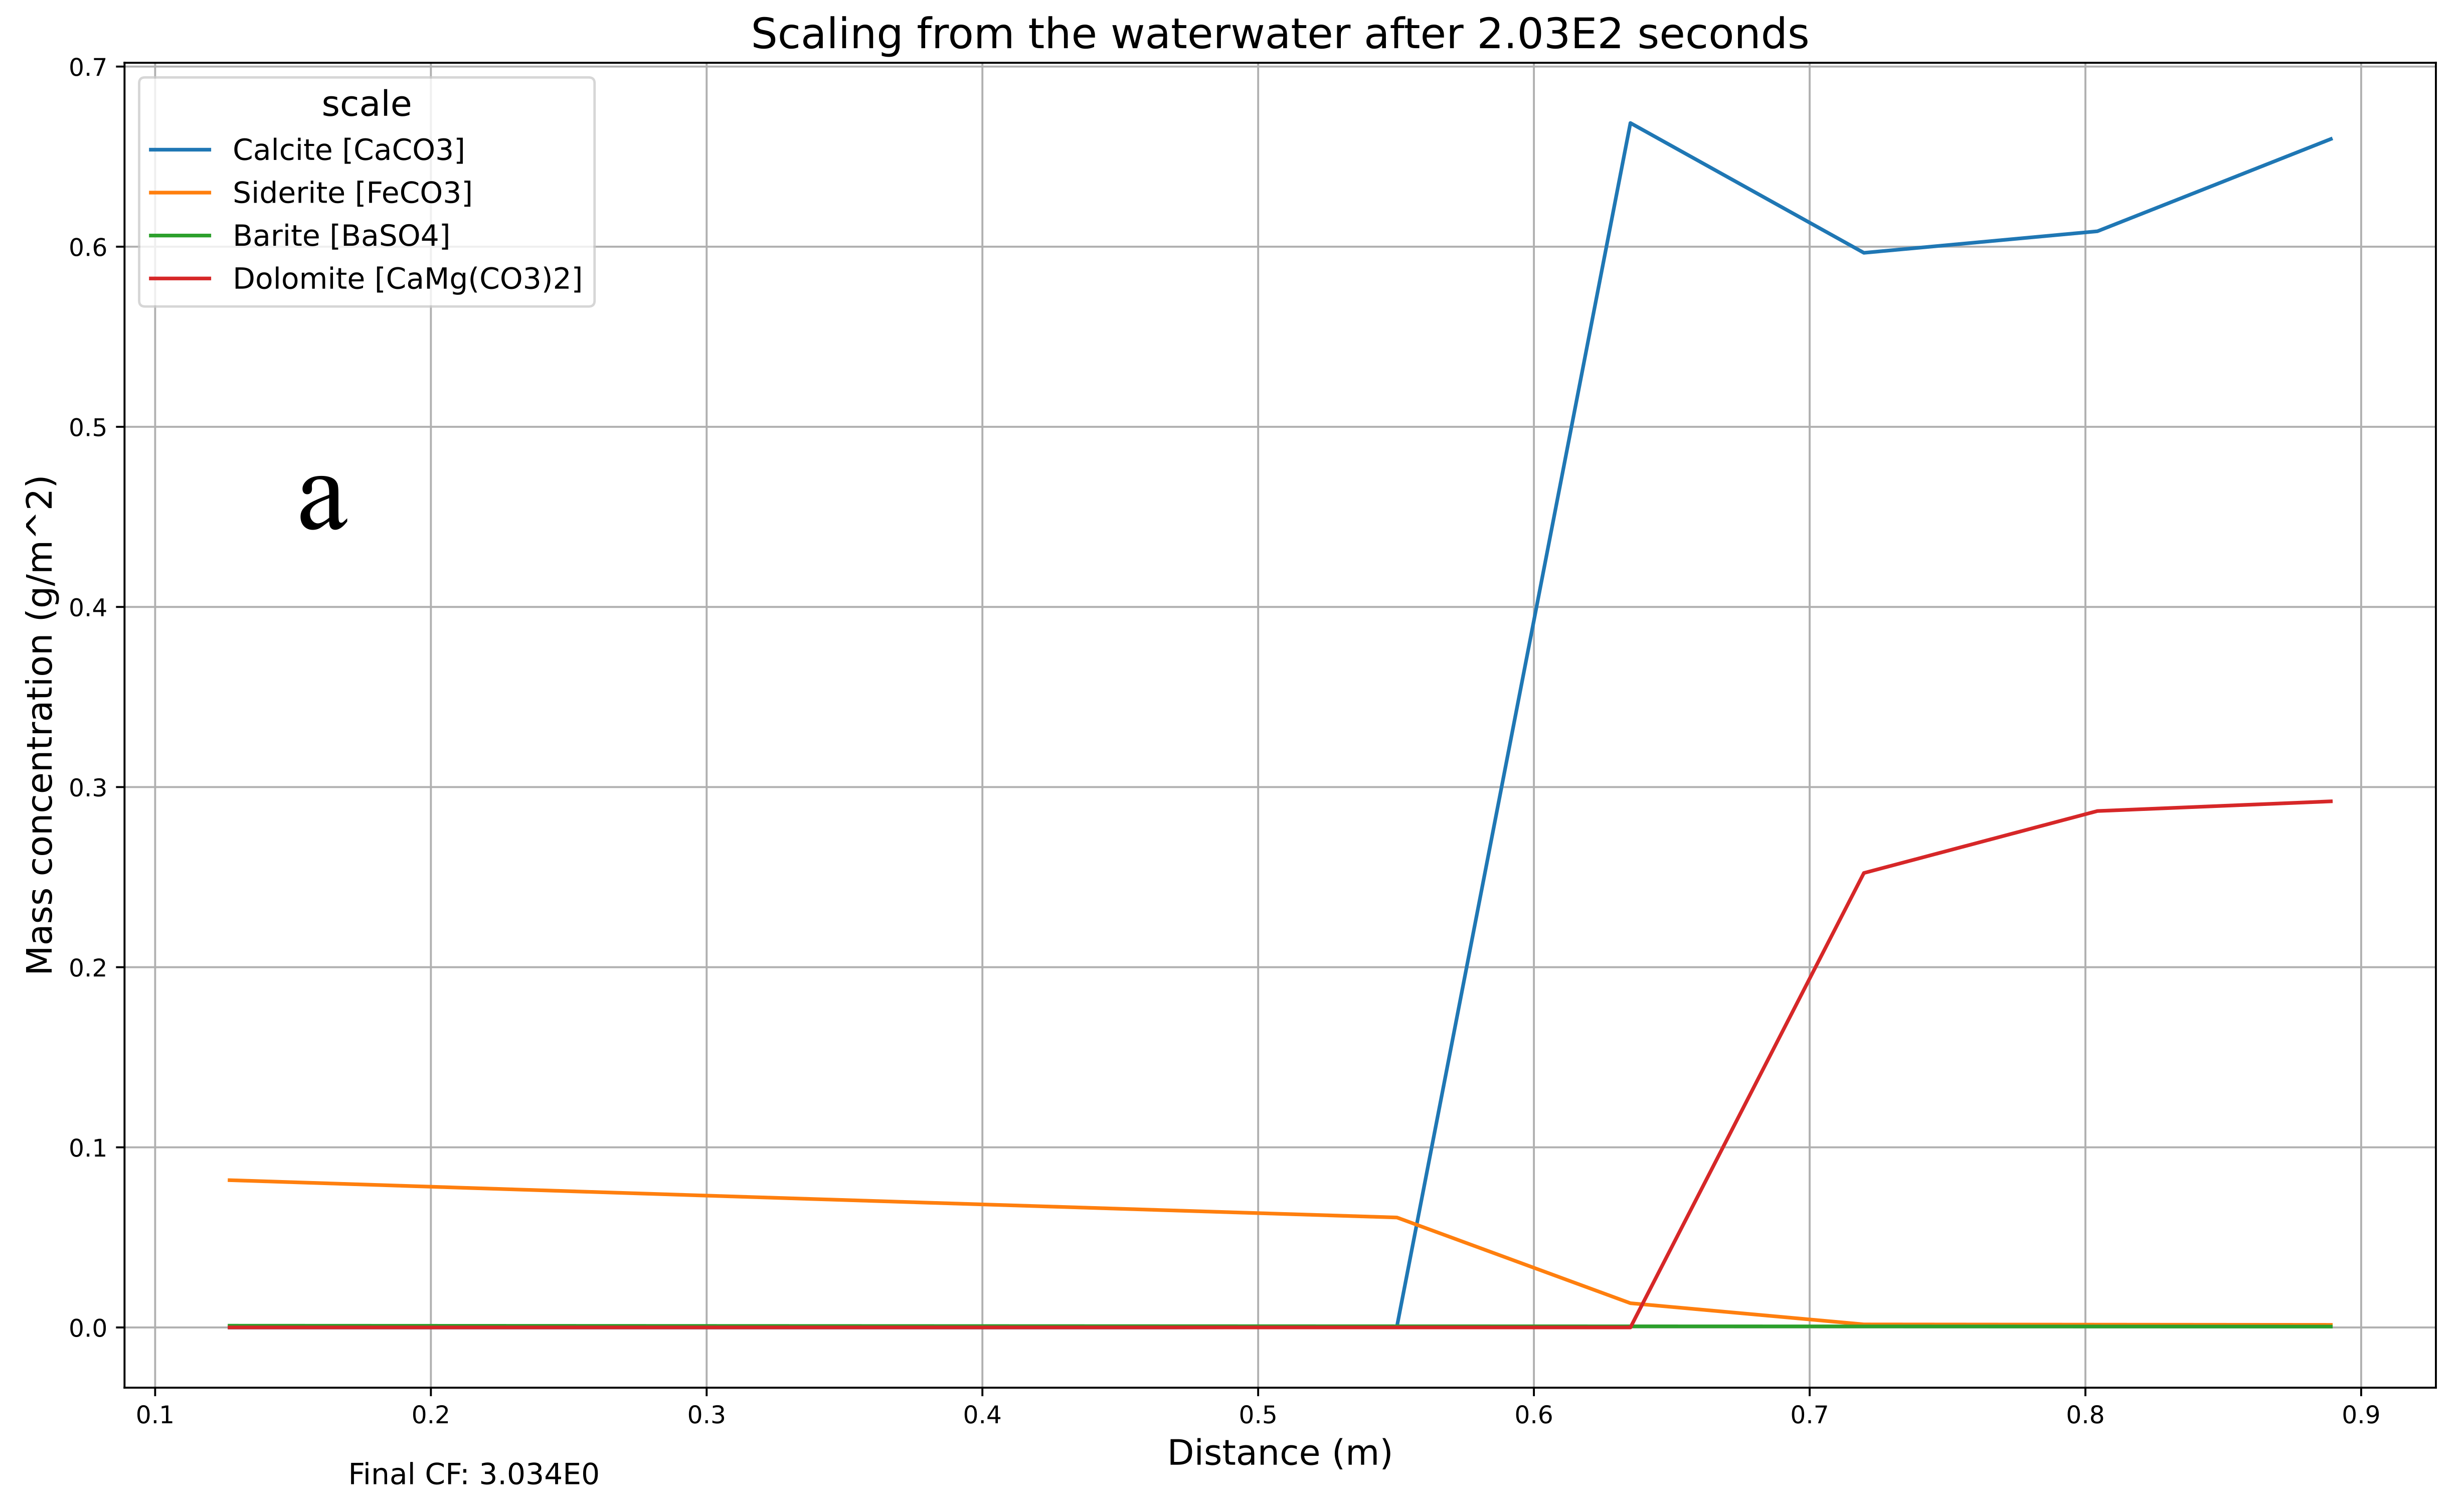
\includegraphics[width=\linewidth]{images/ROSSpy/case_studies/Karabelas_2020_wateq4.png}} \\
        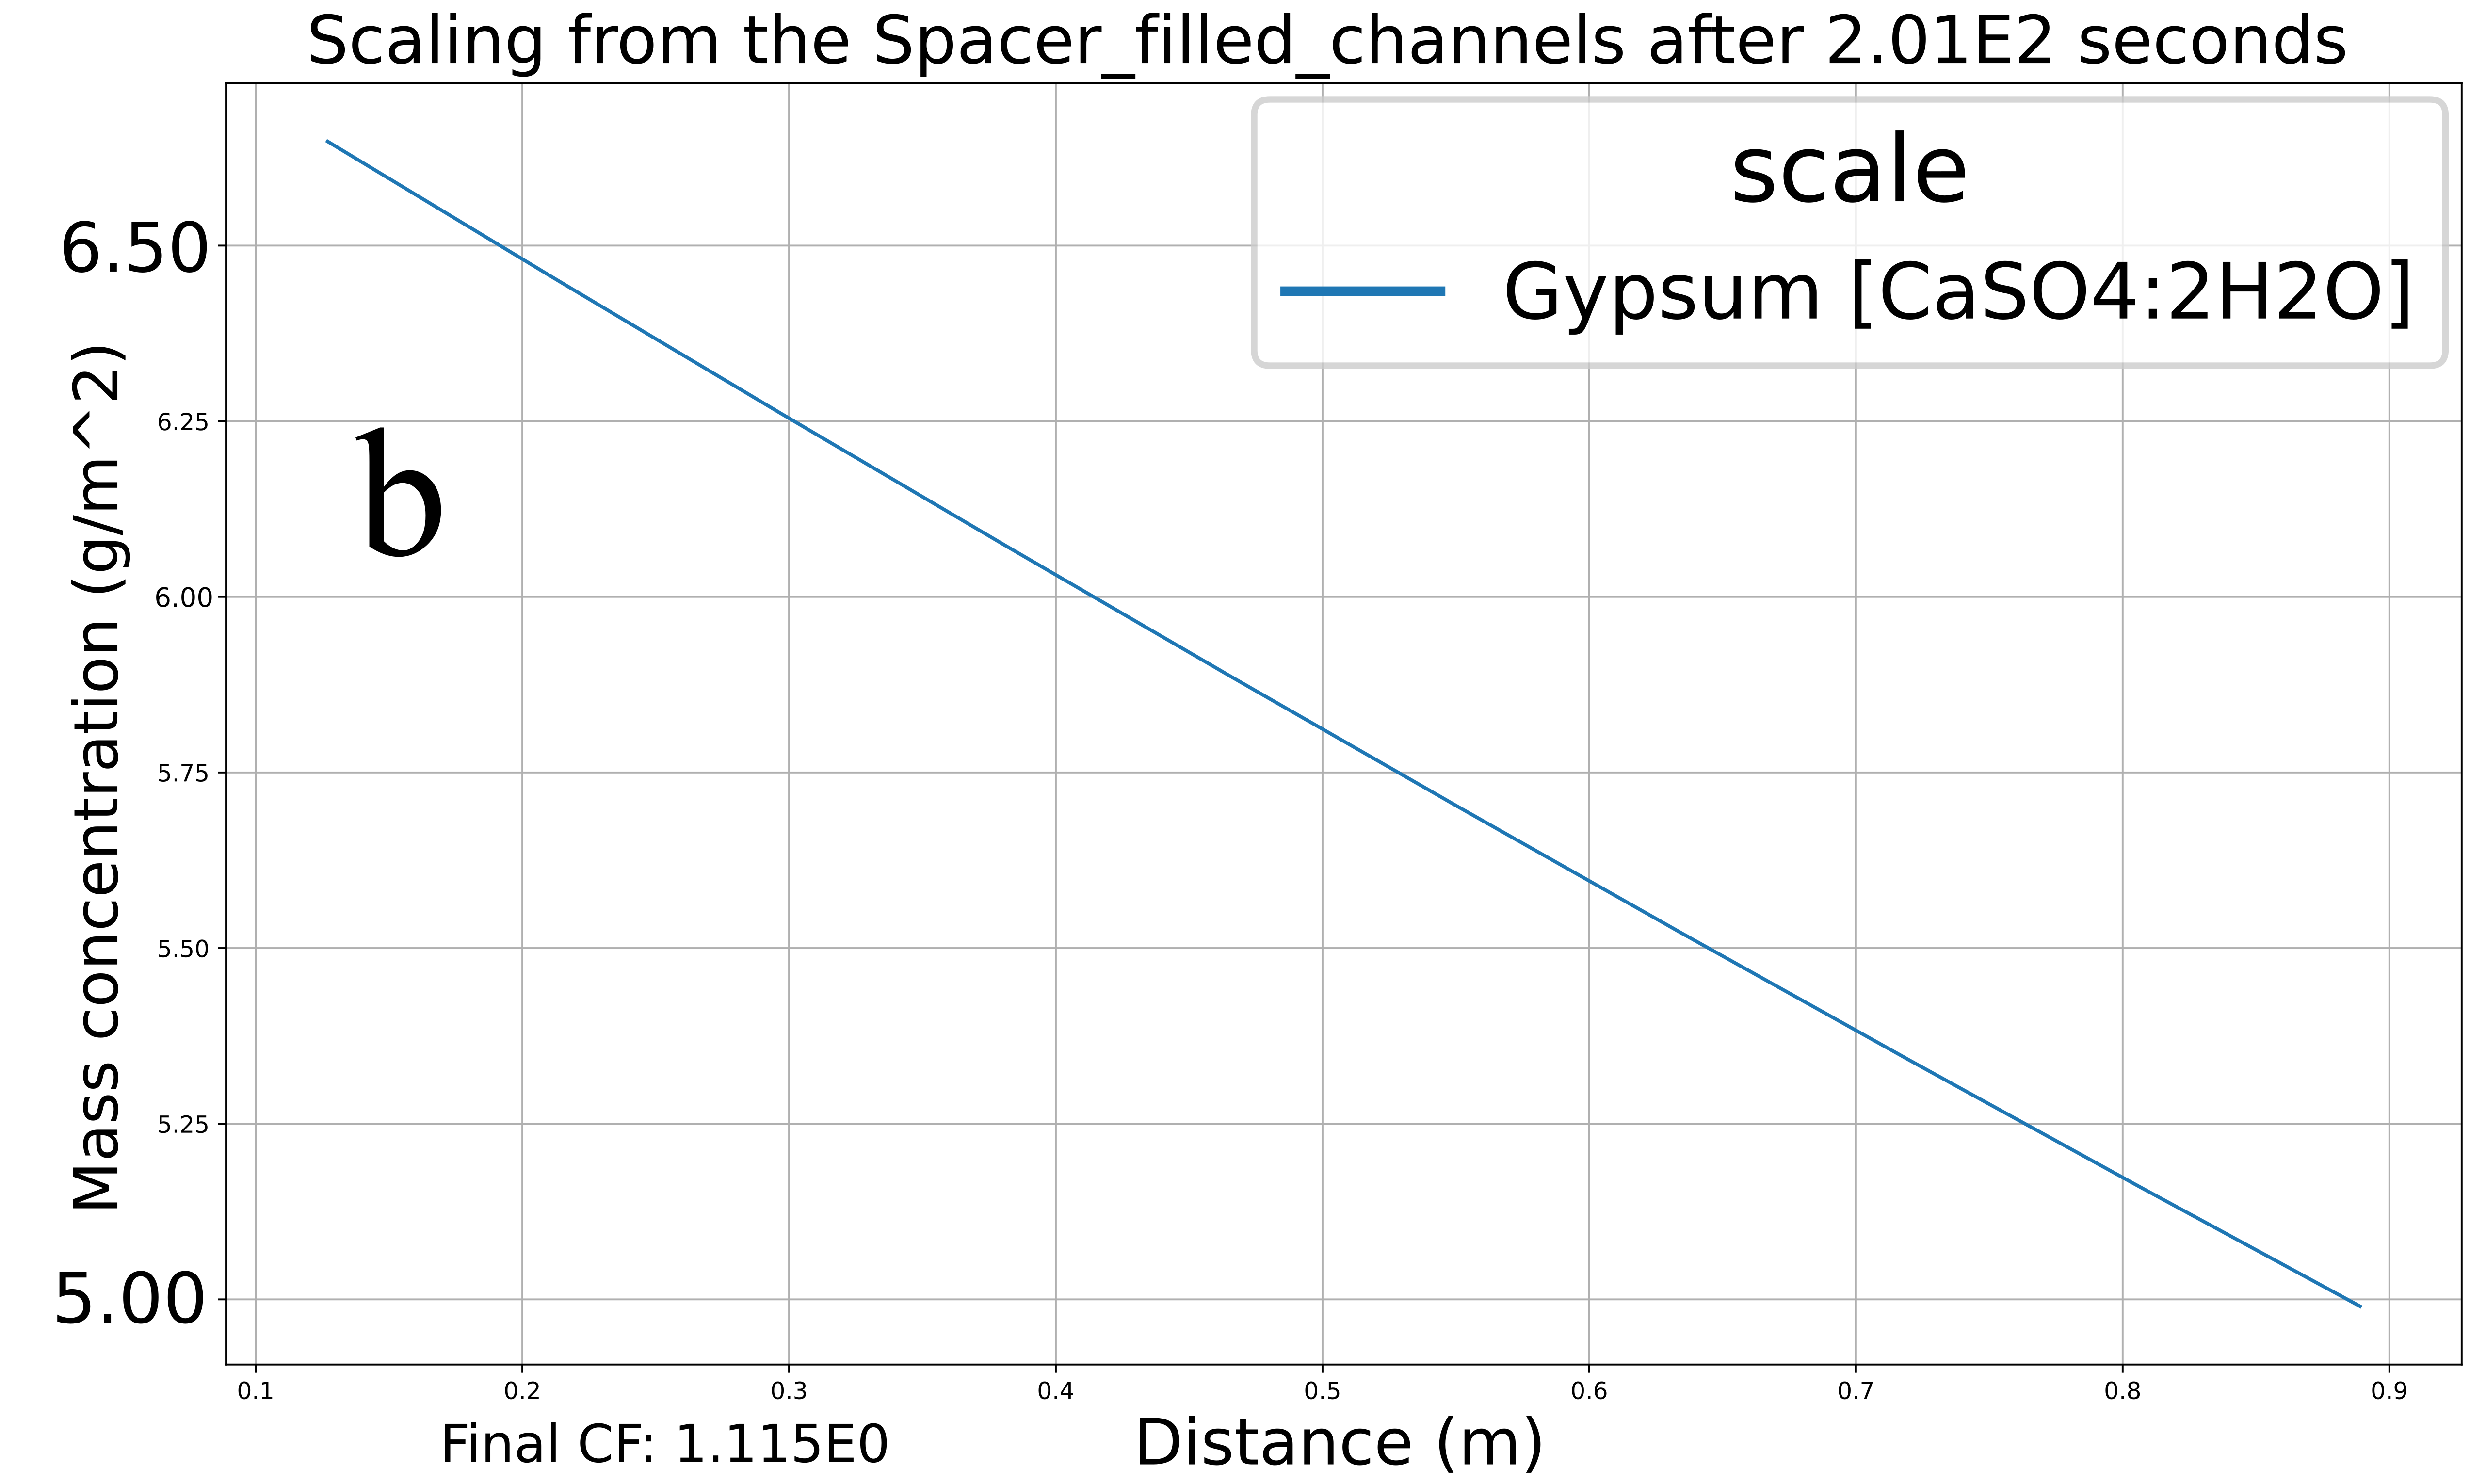
\includegraphics[width=0.49\linewidth]{images/ROSSpy/case_studies/Karabelas_2014_pitzer.png} 
        & 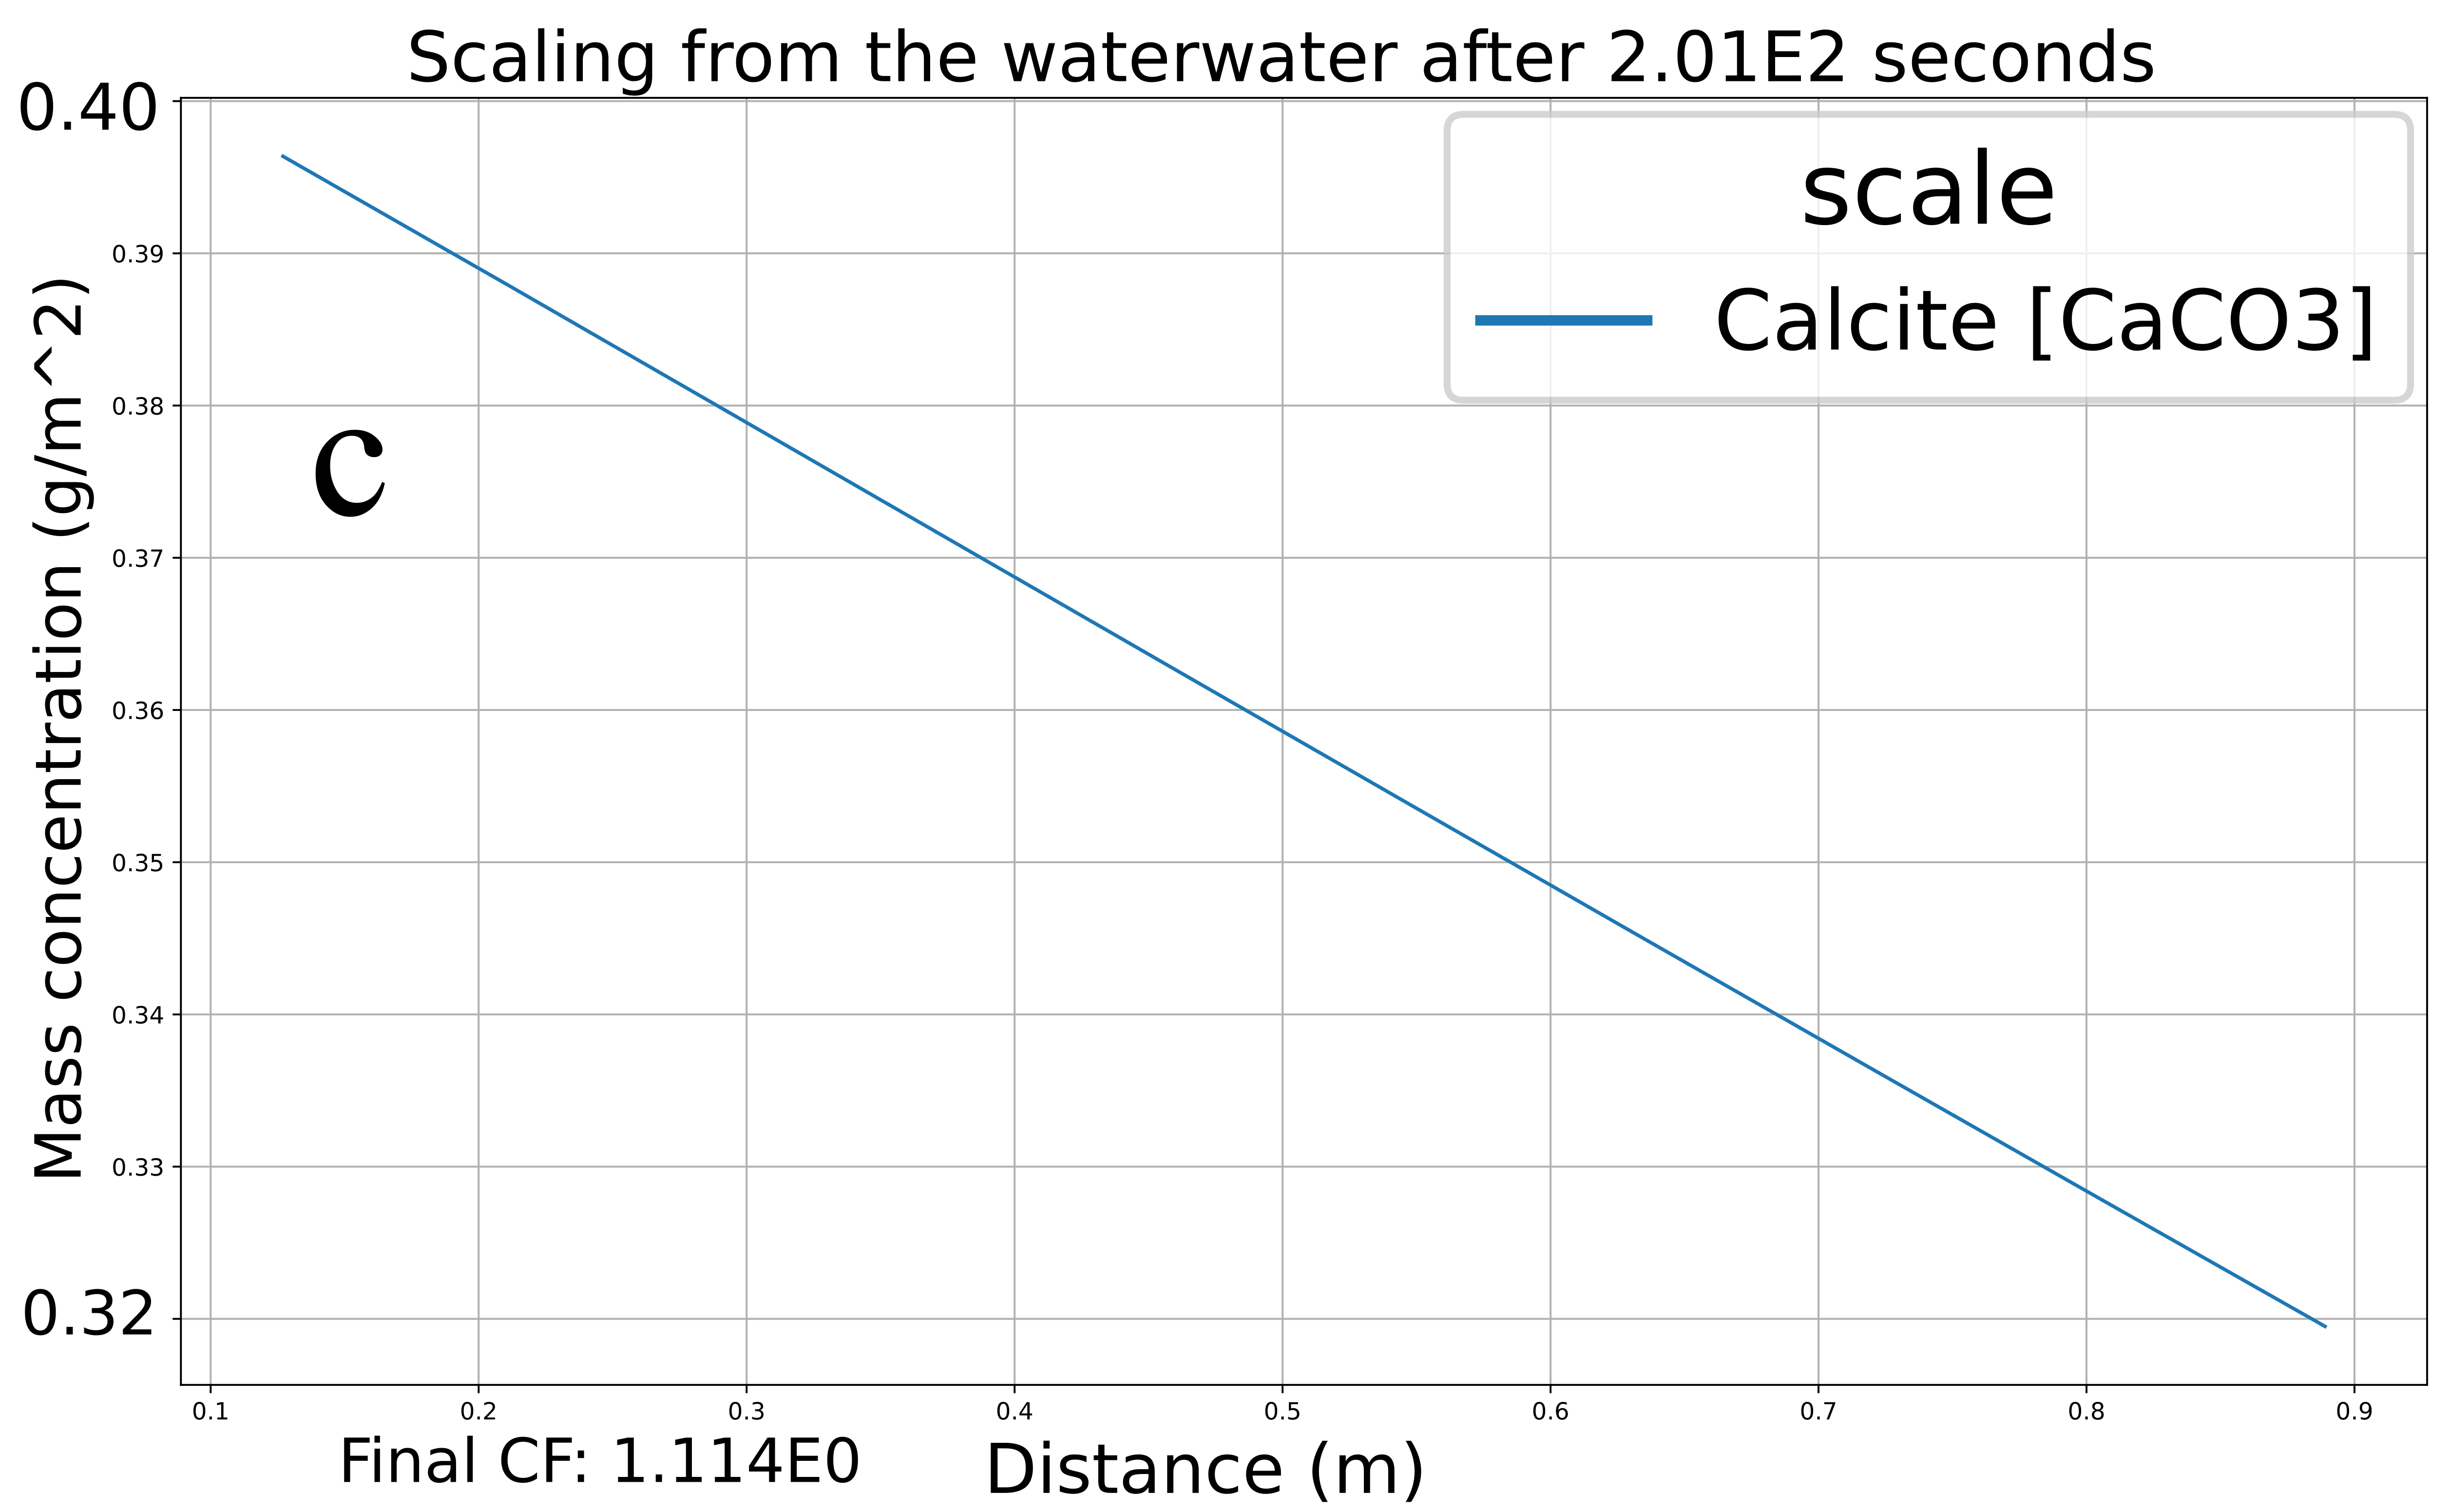
\includegraphics[width=0.49\linewidth]{images/ROSSpy/case_studies/Lee_pitzer.png} \\
    \end{tabular}
    \caption{
        The qualitative validation of scaling for a) multiple minerals from the Karabelas et al., 2020 study; for b) Gypsum in the Karabelas et al., 2014 study; or for c) Calcite in the Lee et al. study.
    }
    \label{qualitative_scaling}
\end{figure}


\section{Sensitivity analyses}
A few sensitivity analyses were conducted with major parameters in the following subsections. Additional sensitivity analyses of lesser parameters are presented in the Supporting Information.

\subsection{Database section}
The parameterized PHREEQ database both quantitatively and qualitatively influences the scaling predictions of ROSSpy. These databases crucially contain all of the kinetic and thermodynamic information for each precipitation interaction, and use different geochemical calculations according to the chemical model -- e.g. Pitzer, Debye-H\"uckel, and Davies. Section 7 of the Supporting Information elaborates these databases and their underlying chemical models further. The Pitzer model \cite{Pitzer1973ThermodynamicsEquations,Pitzer1974ThermodynamicsElectrolytes} is touted as being supremely accurate for $CF \in [1,6]$ systems, which corresponds to the brine concentration range after seawater desalination \cite{VandeLisdonk2001PredictionSystems,Sheikholeslami2004AssessmentUnits,Mohammad2007PredictionMembranes}; however, the narrow range of accepted ions and minerals by the Pitzer model may justify using databases, such as wateq4, that use other chemical models for complex feed sources. 

A standard simulation of the Red Sea as the feed source was conducted with each of the PHREEQC databases. The simulation with the $\frac{4}{13}$ of the databases -- $Amm$, $Core10$, $LLNL$, and $Minteq.v4$ -- failed to numerically converge, and the variability in the predictions is illustrated in Figure \ref{database_selection}. User intuition and review of the PHREEQC User's Manual is evidently important when selecting the PHREEQC database for a simulation, where the chemical model and scope of database content significantly change scaling predictions.

\begin{figure}[h]
    \centering
    \begin{tabular}{c|c}
        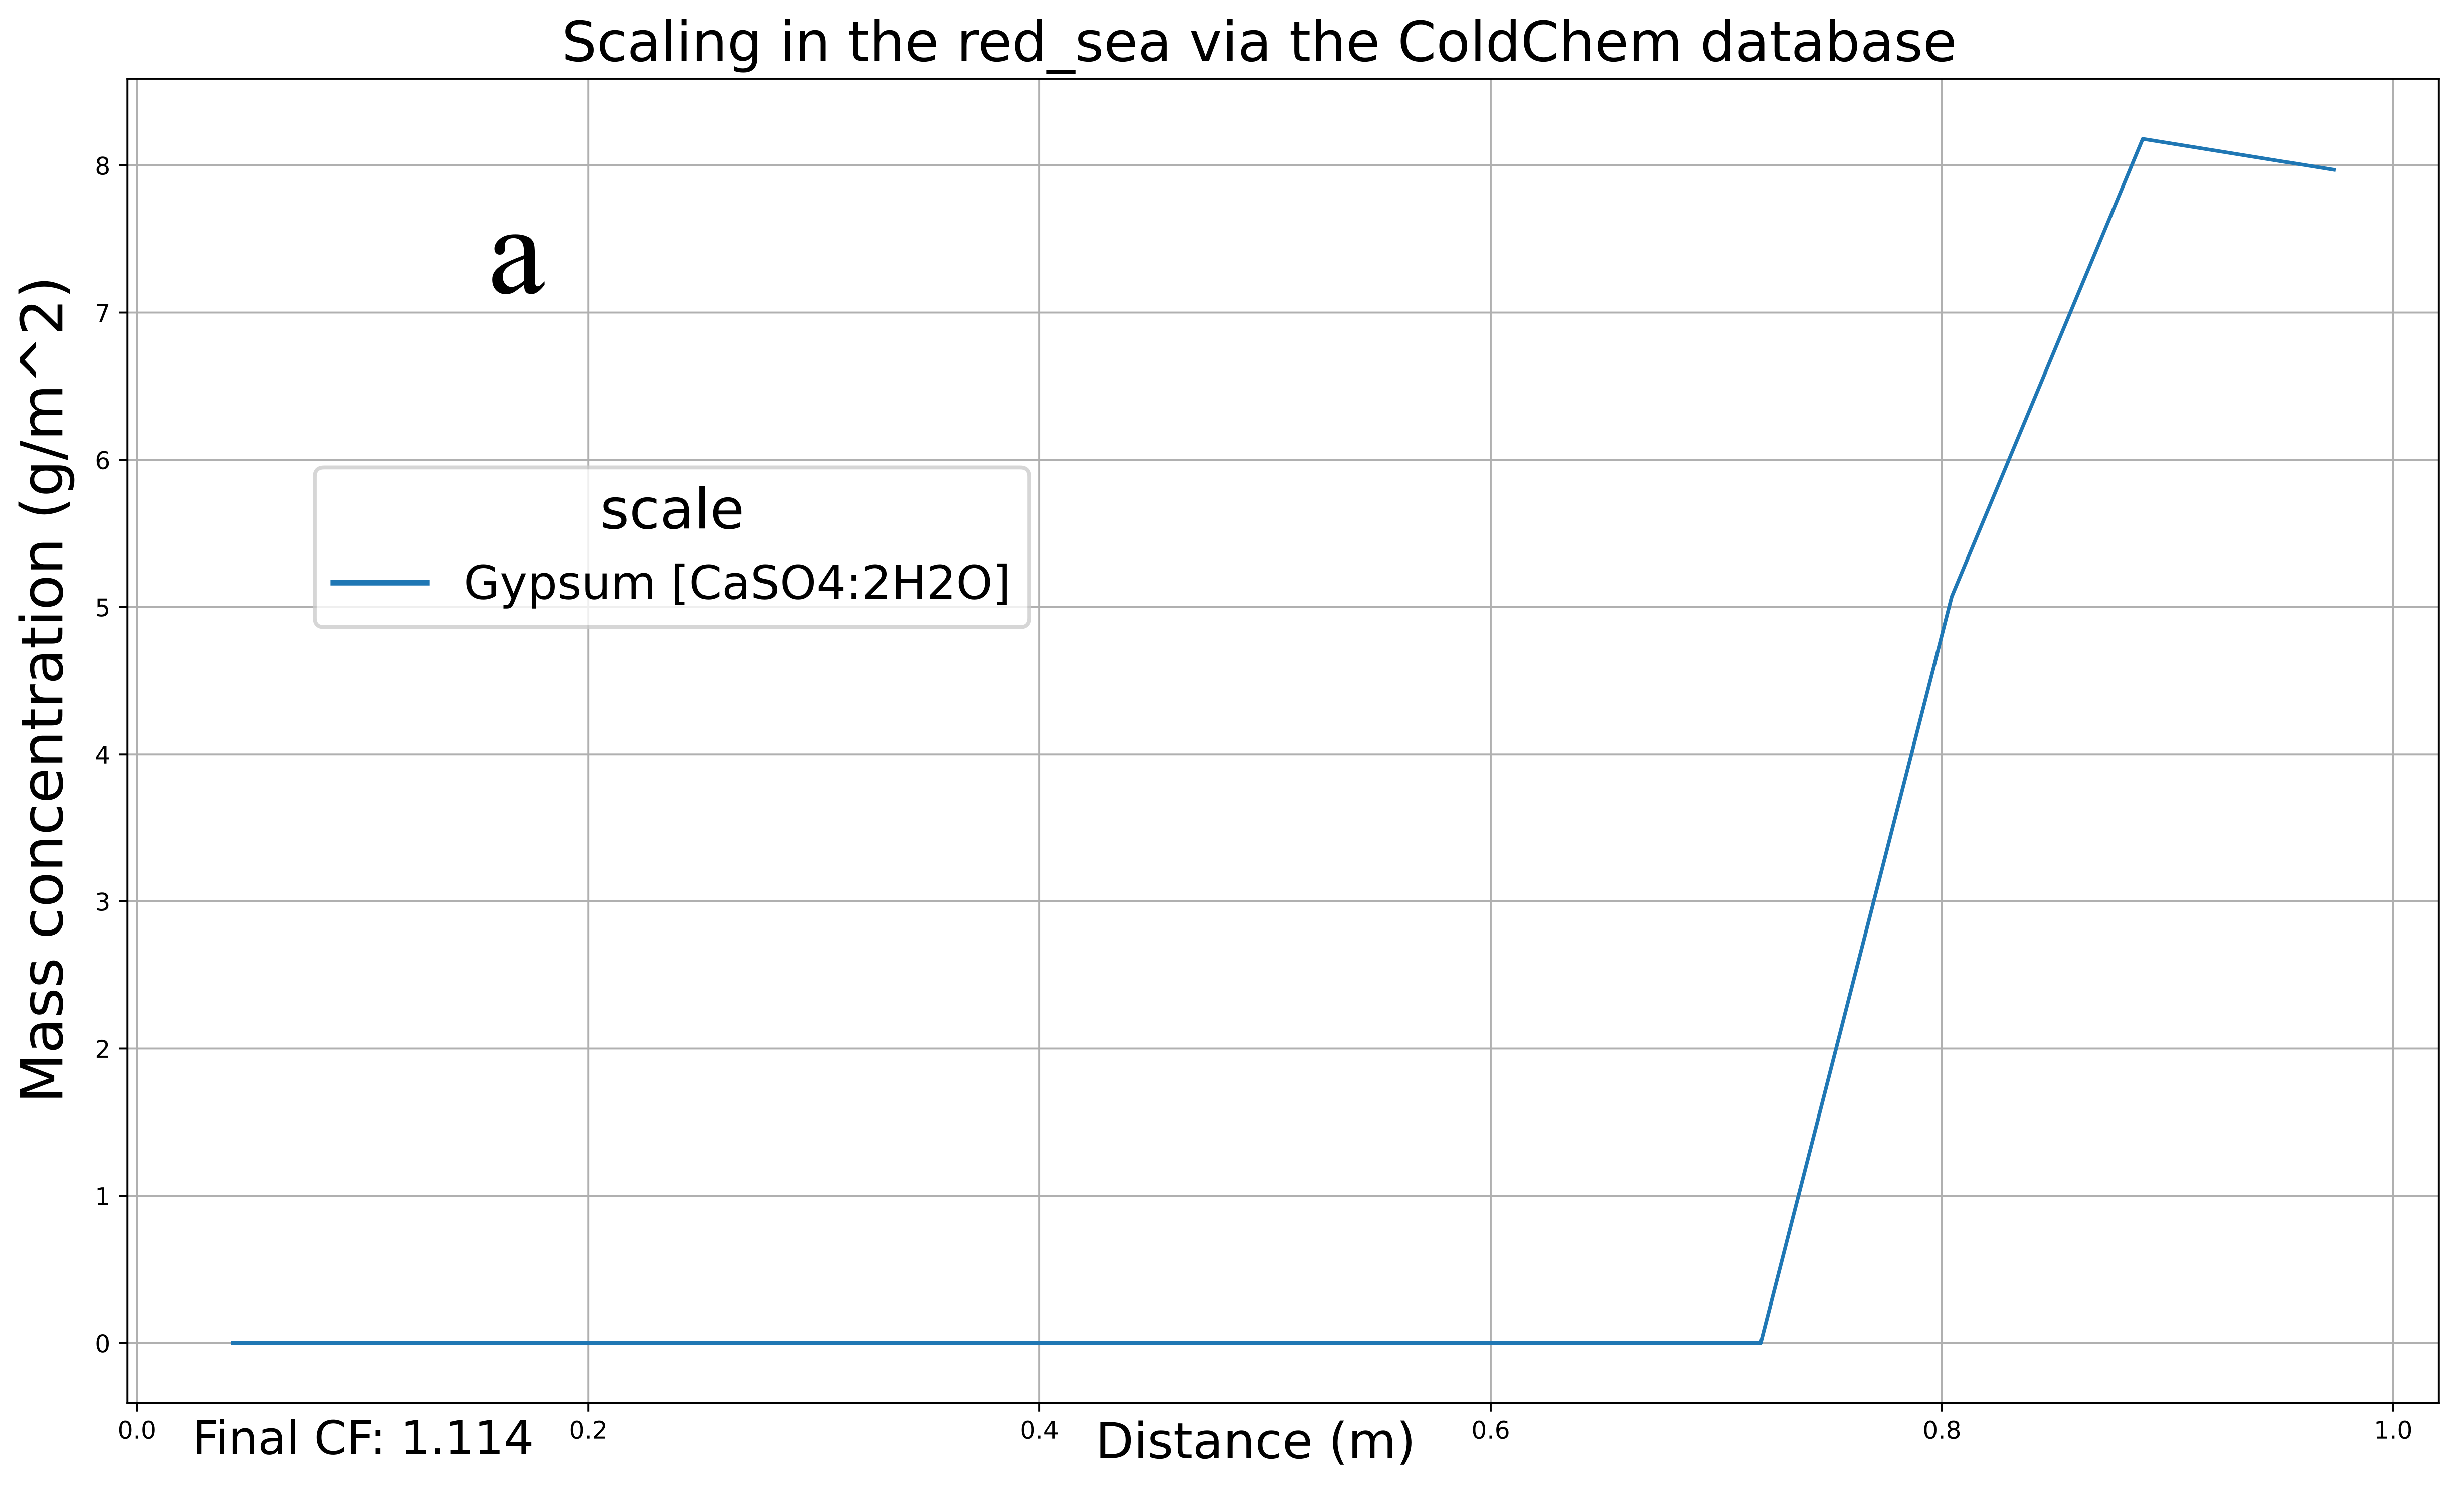
\includegraphics[width=0.49\textwidth]{images/ROSSpy/sensitivity_analyses/databases/ColdChem.png} 
        & 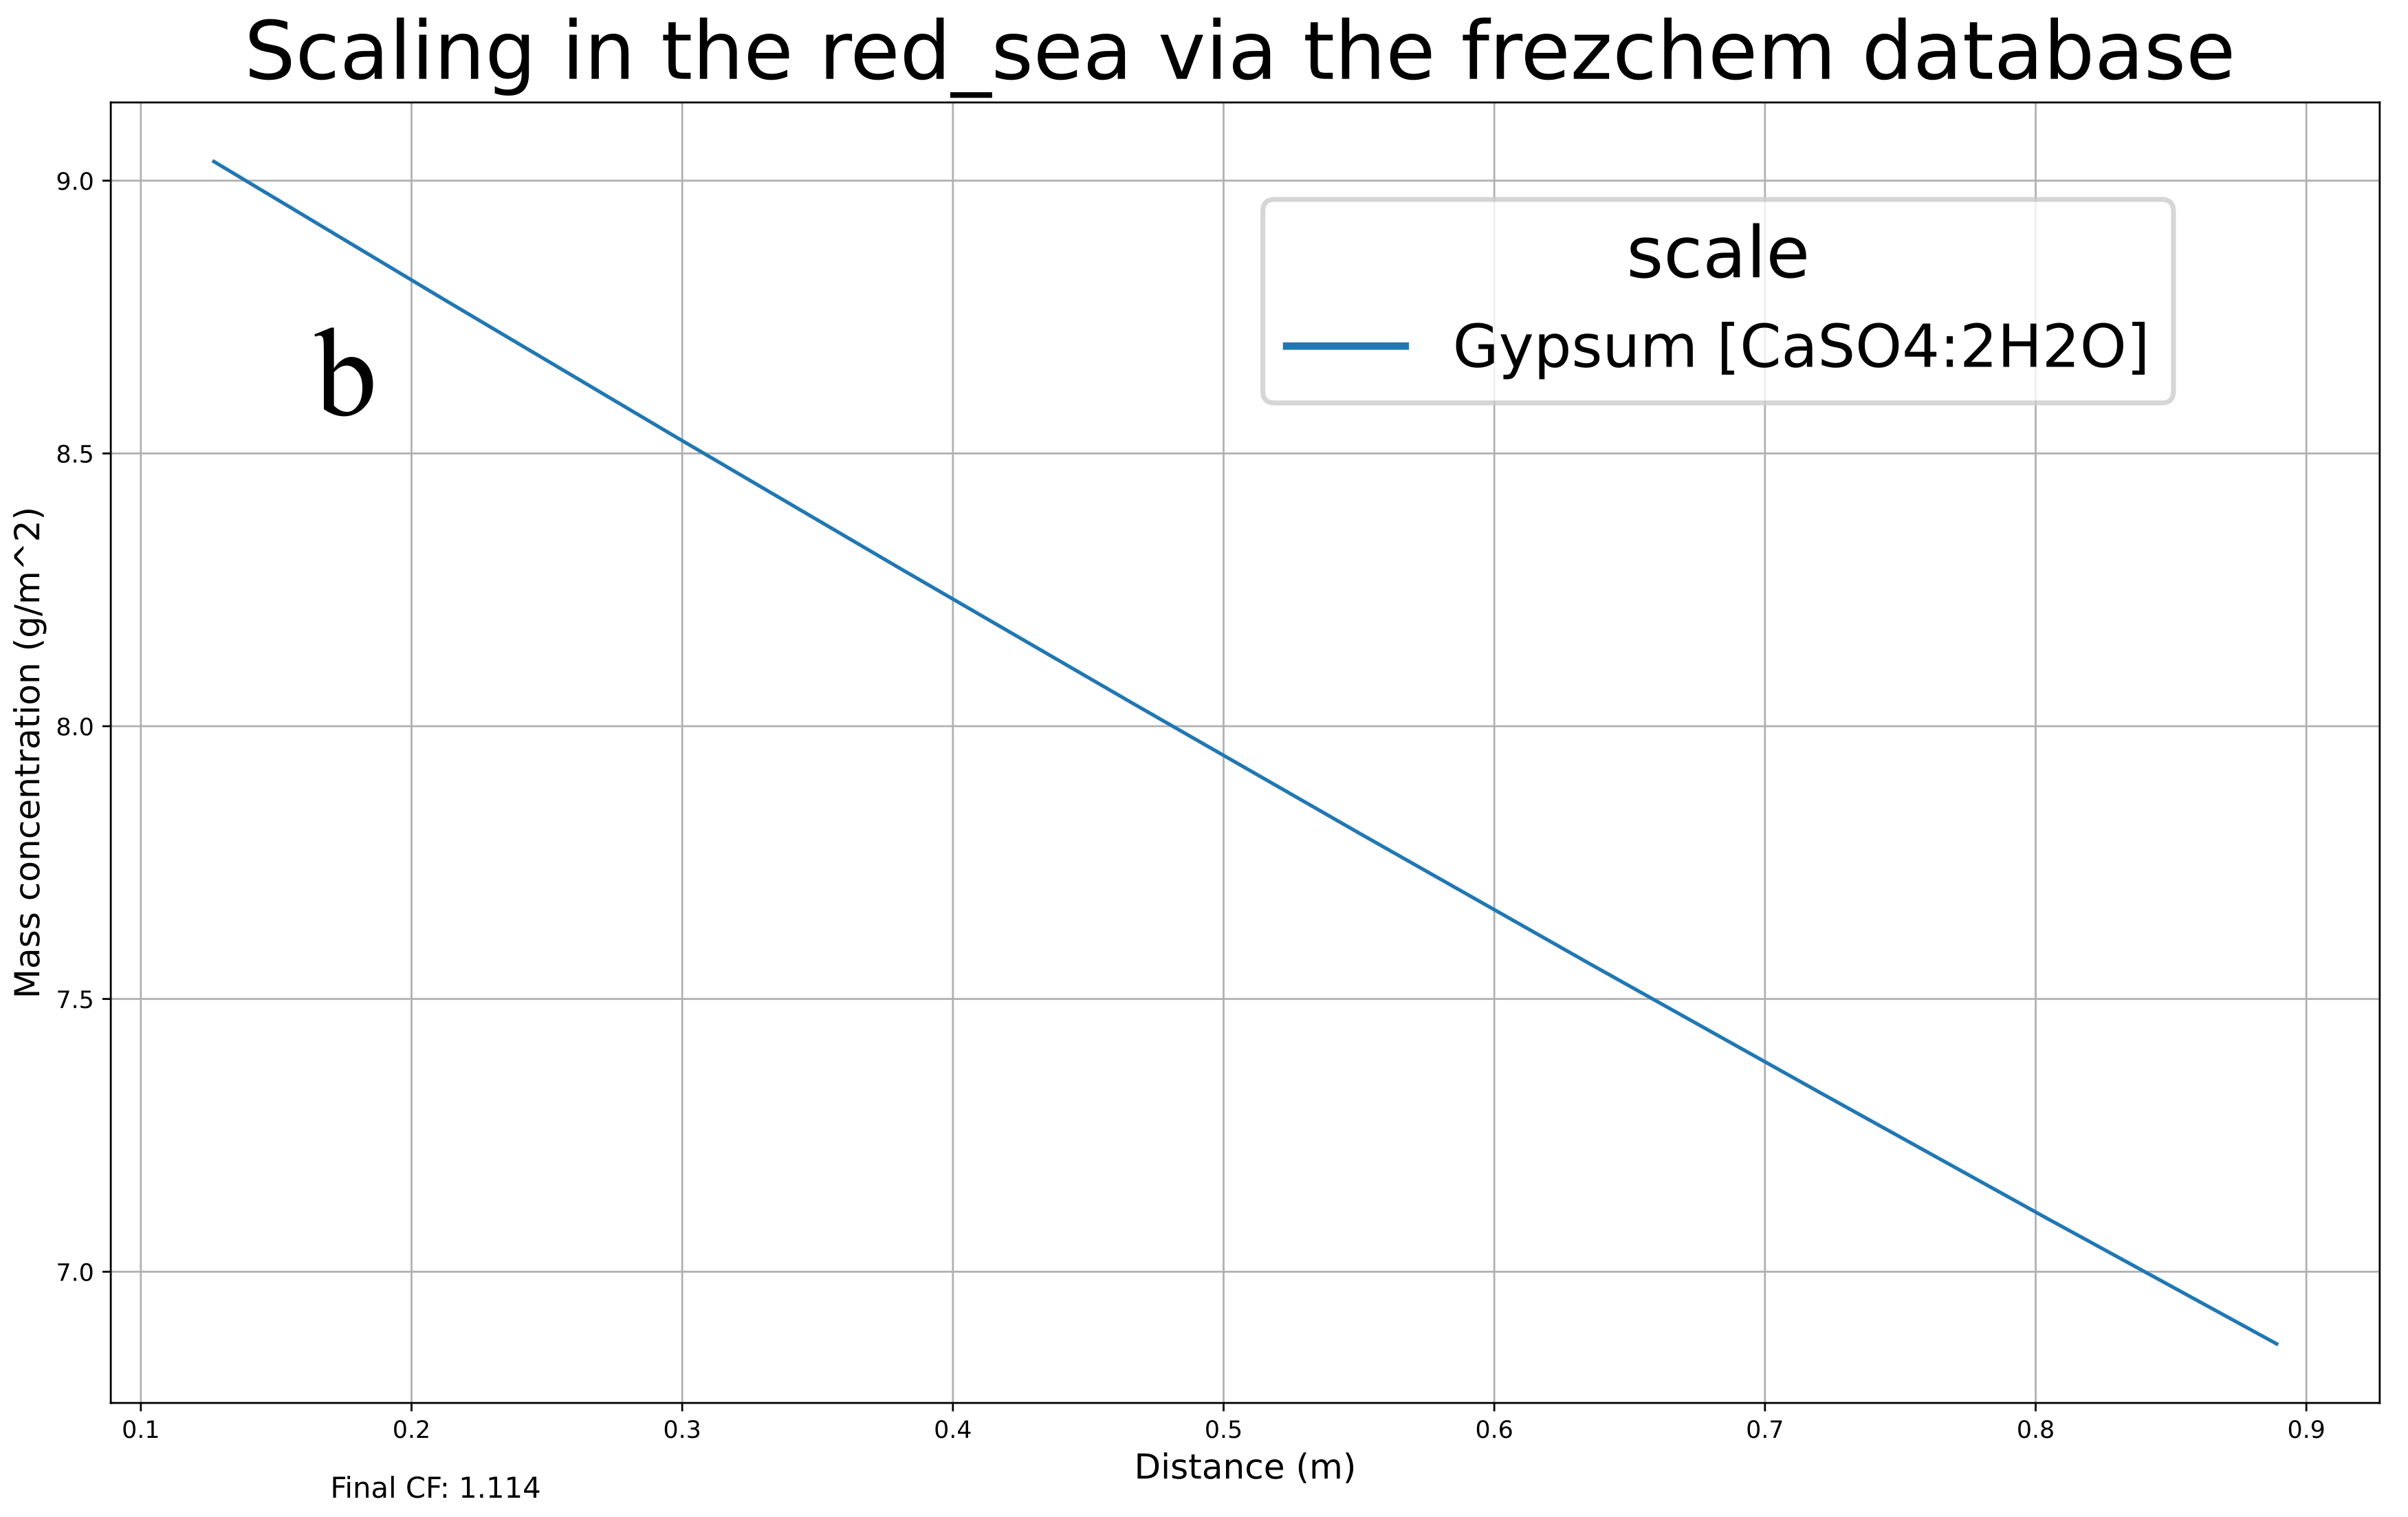
\includegraphics[width=0.49\textwidth]{images/ROSSpy/sensitivity_analyses/databases/FreezChem.png} \\ \midrule 
        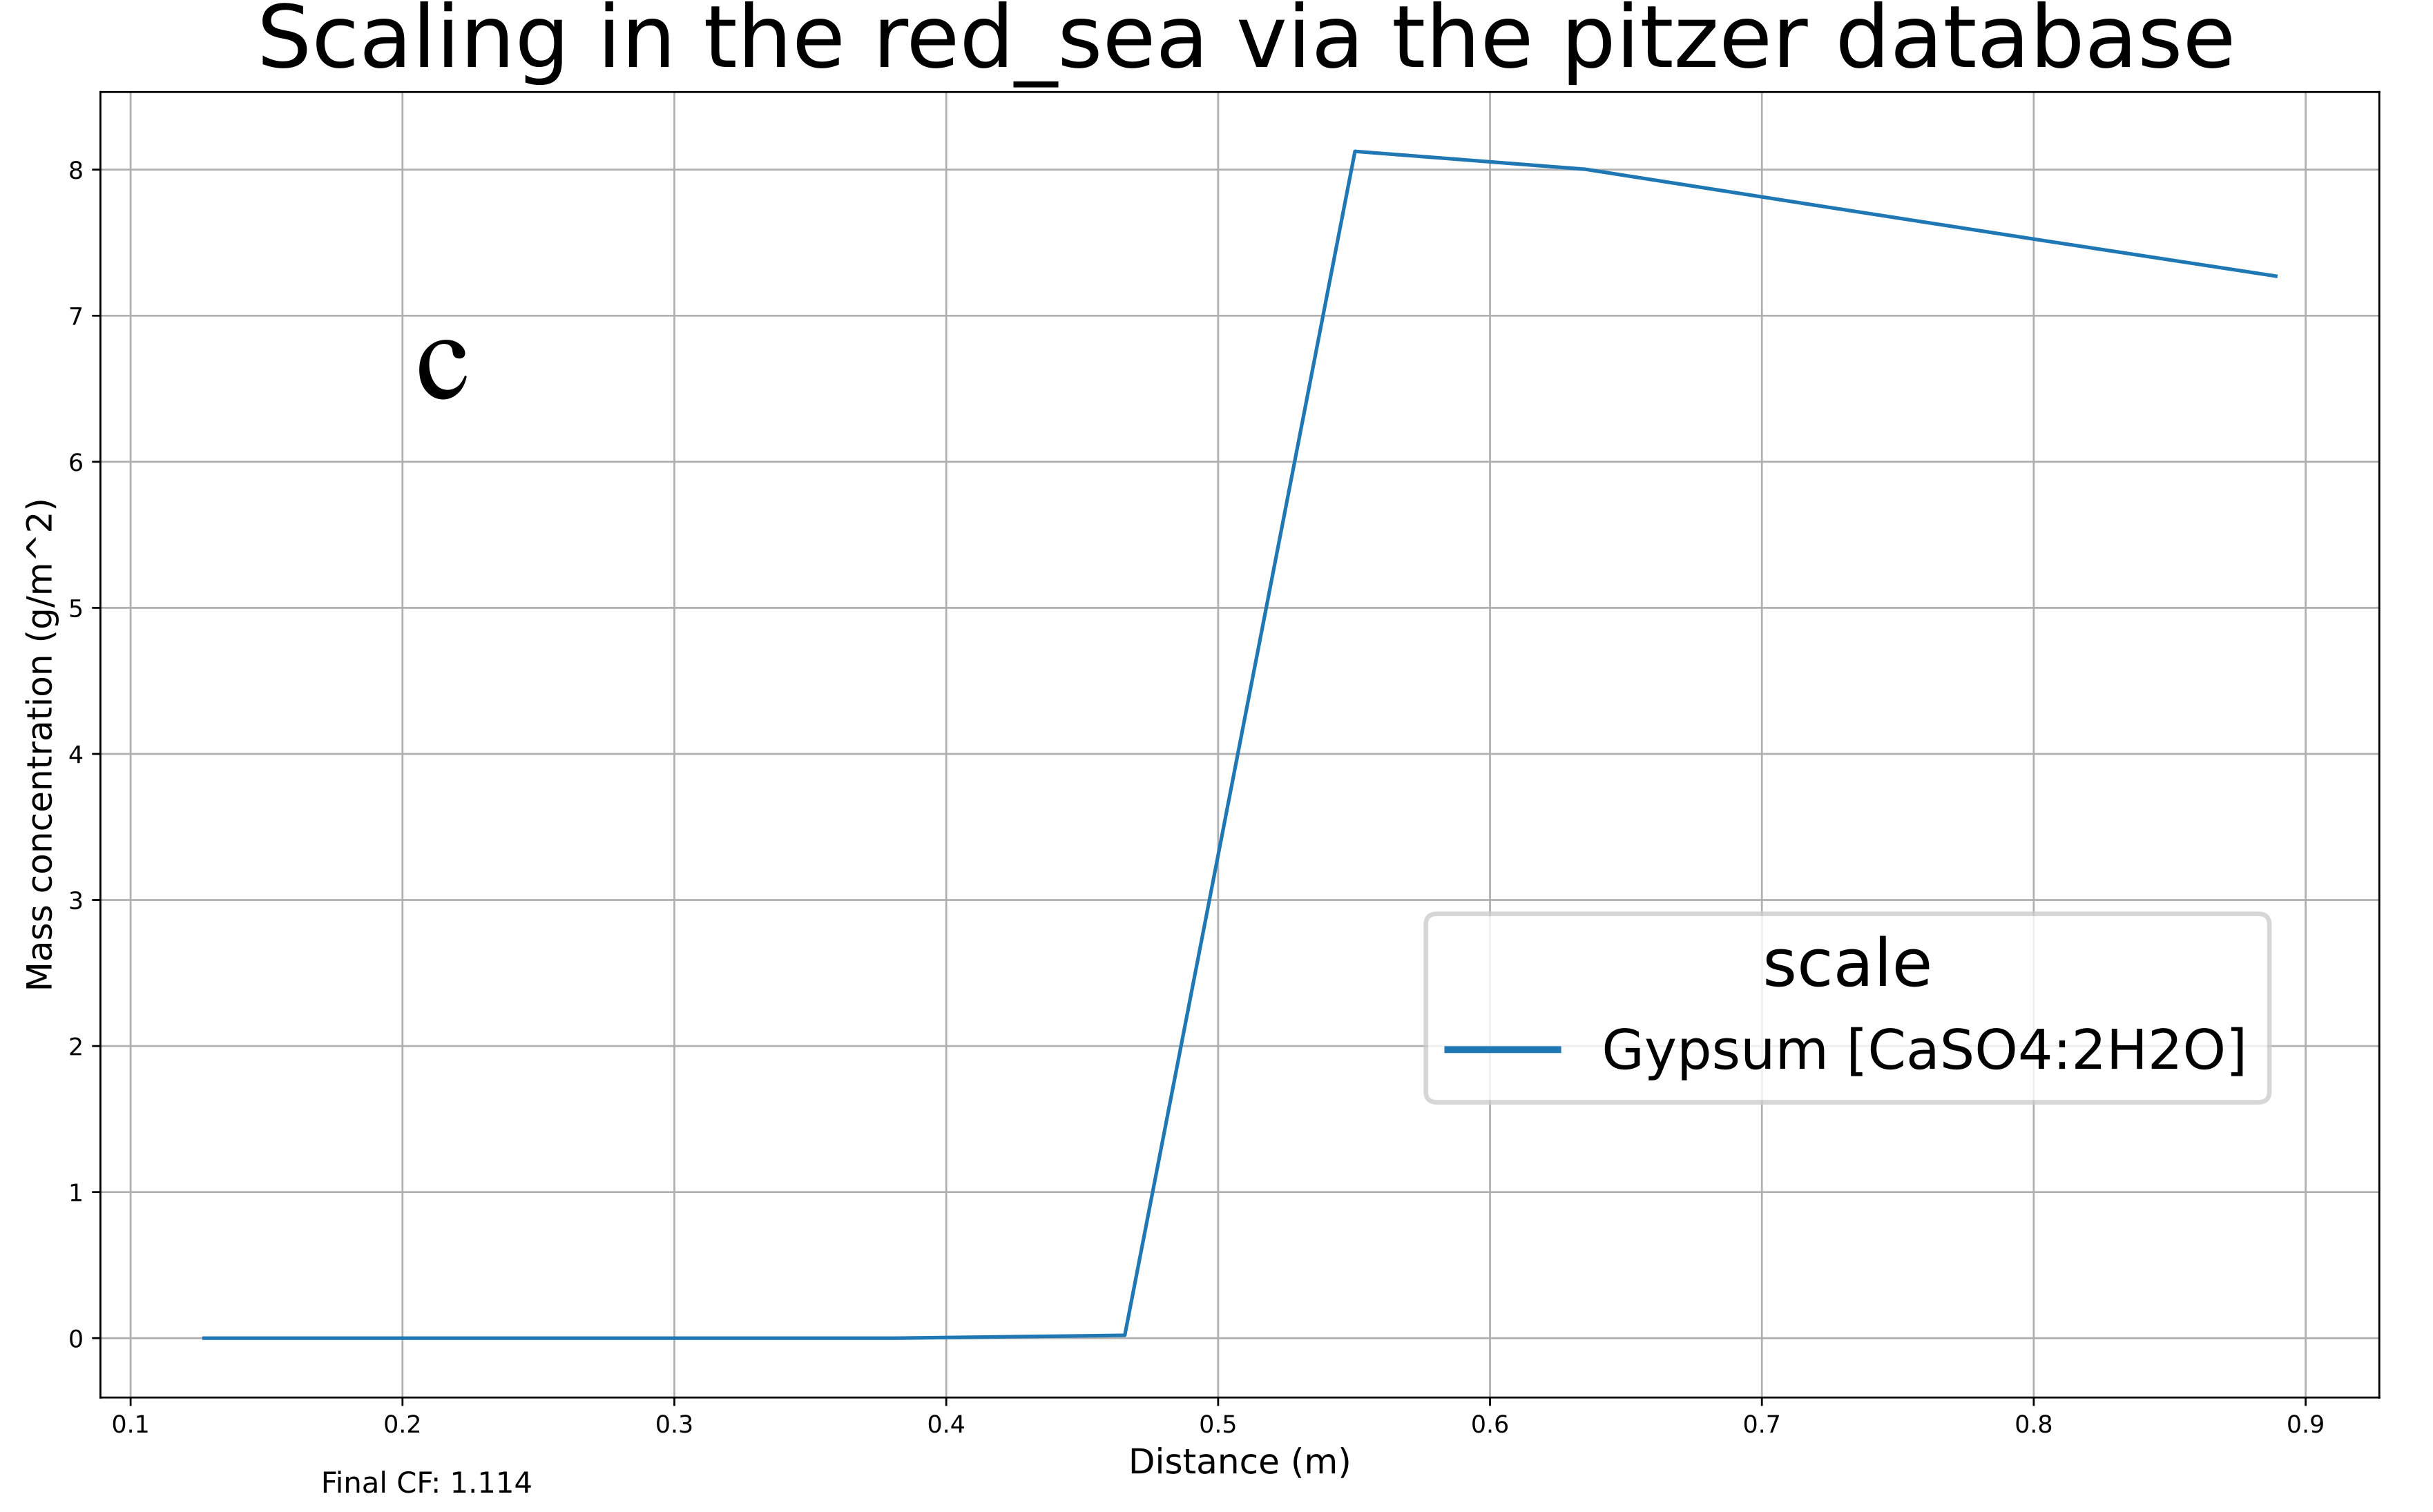
\includegraphics[width=0.49\textwidth]{images/ROSSpy/sensitivity_analyses/databases/Pitzer.png} 
        & 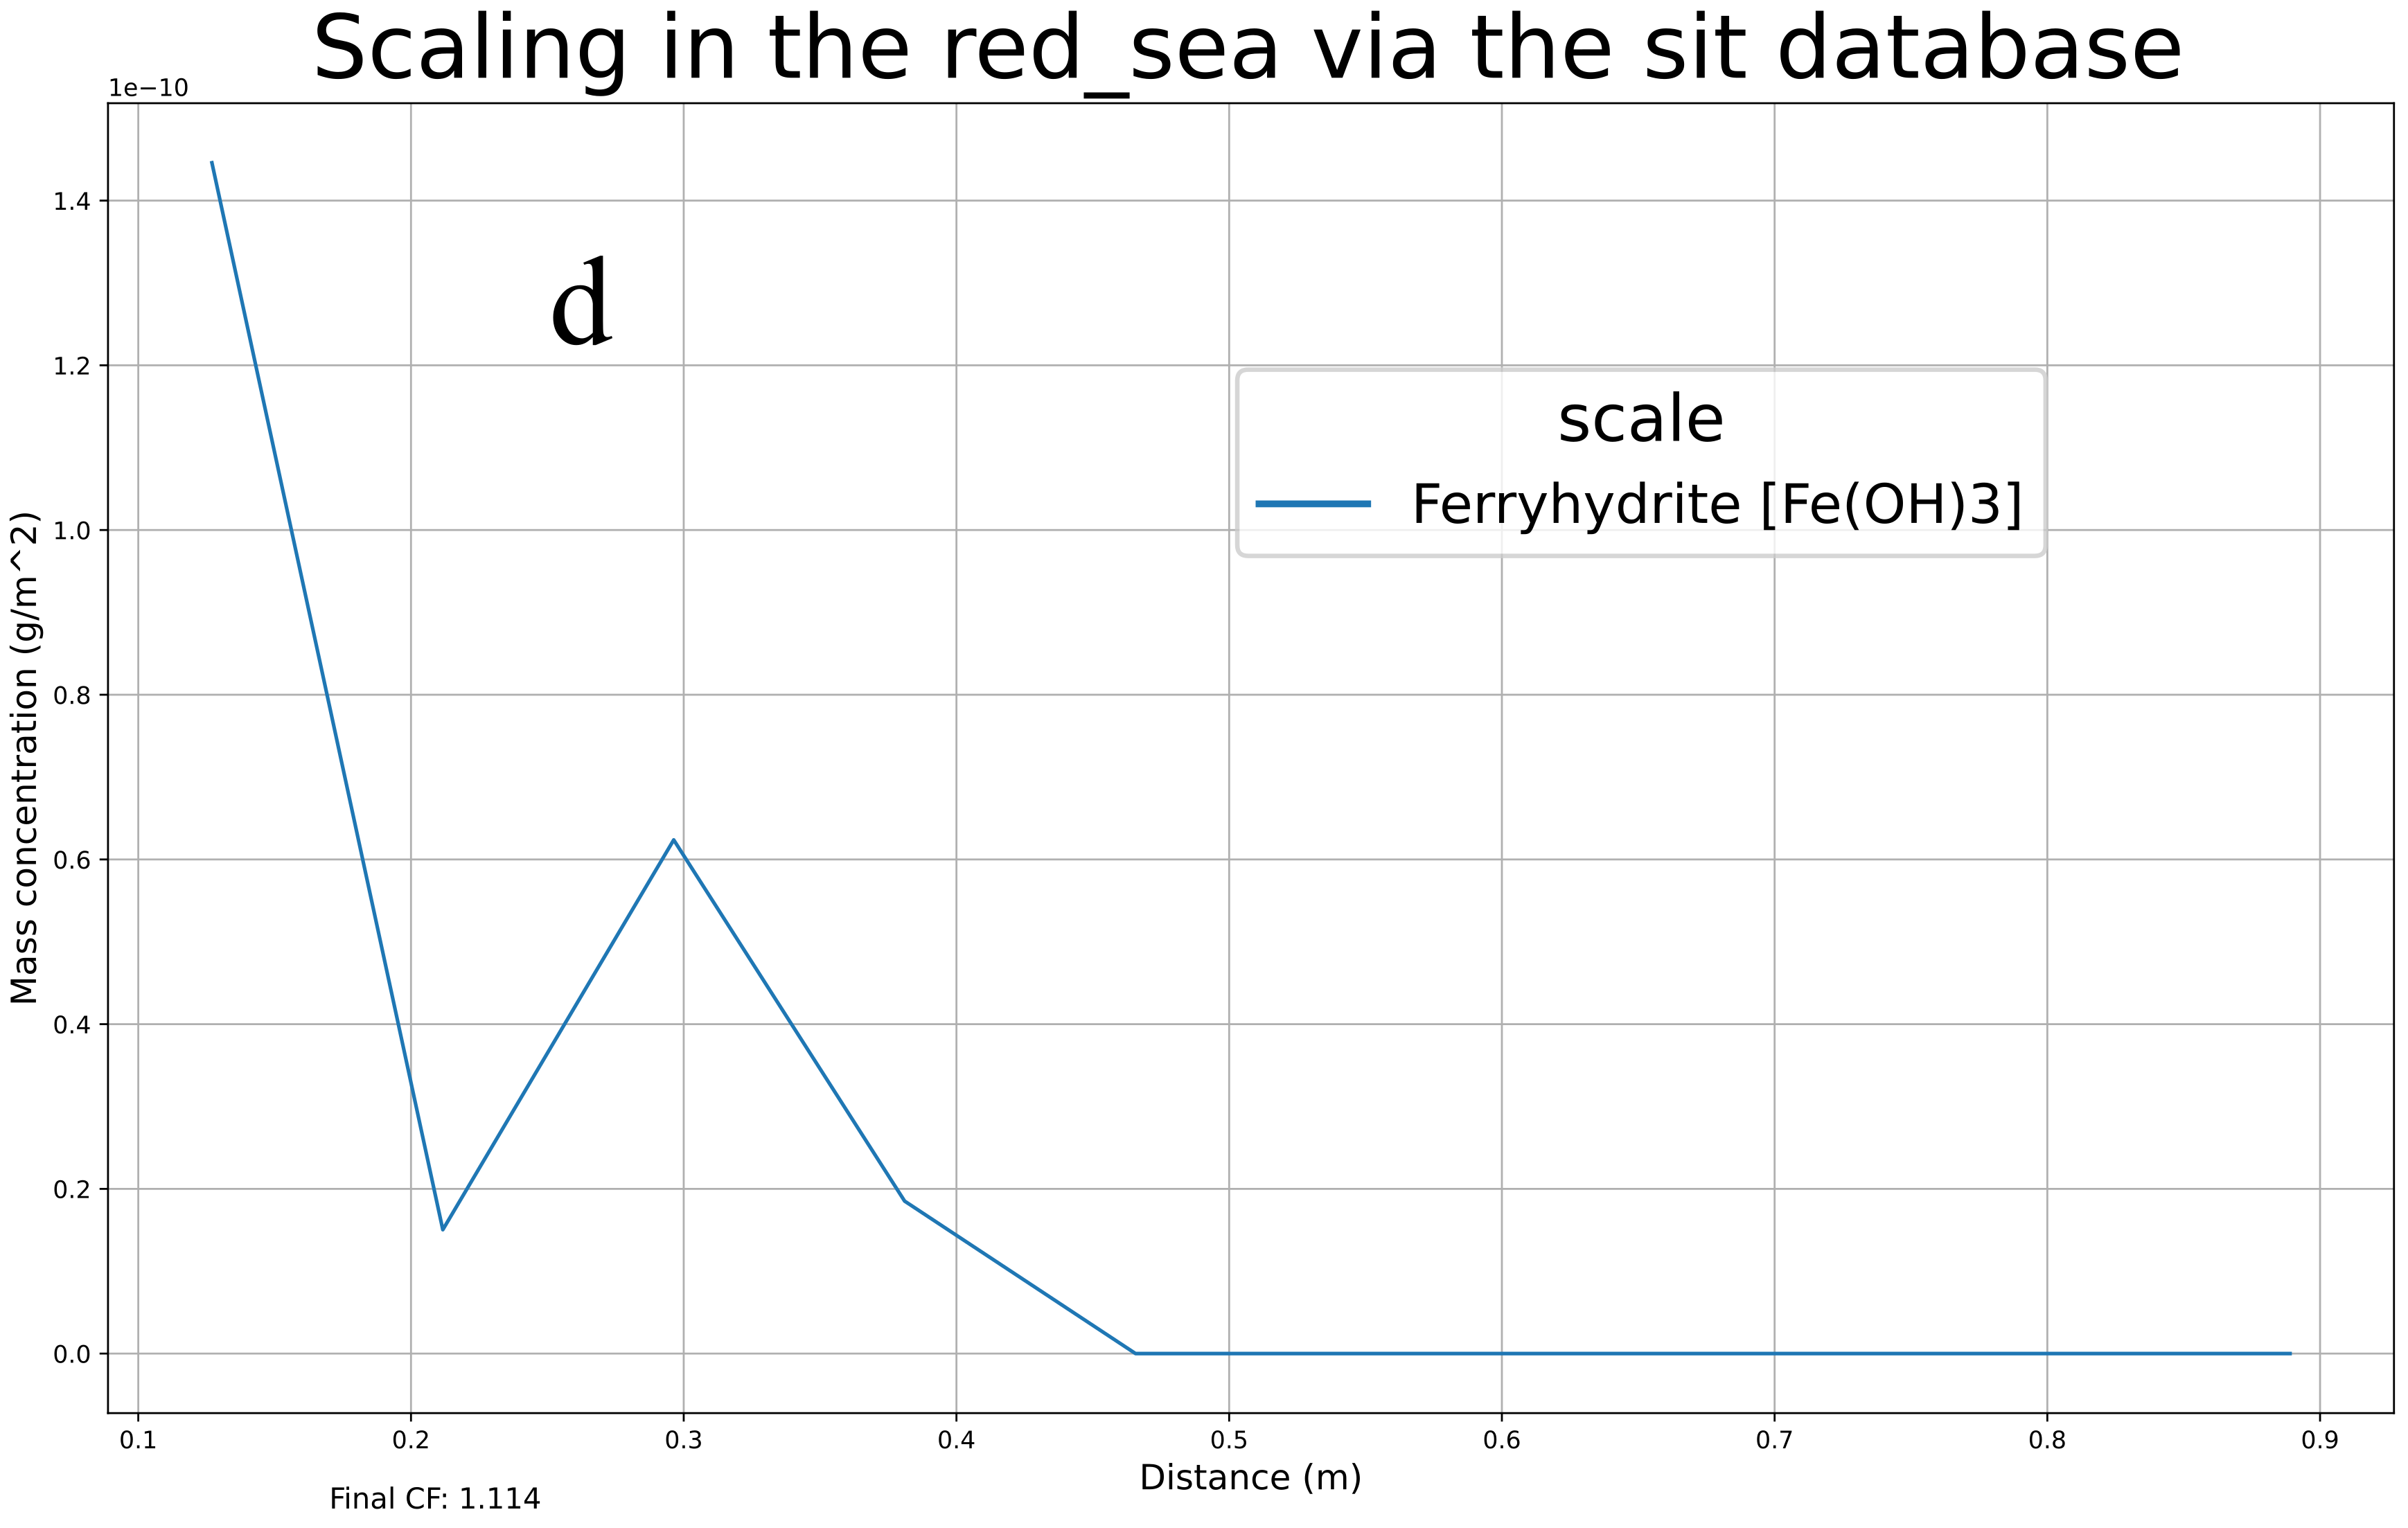
\includegraphics[width=0.49\textwidth]{images/ROSSpy/sensitivity_analyses/databases/Sit.png} 
        \\ \bottomrule
    \end{tabular}
    \caption{
        Scaling predictions from the a) ColdChem, b) FreezChem, c) Pitzer, and d) Sit databases, with otherwise identical simulation parameters.
    }
    \label{database_selection}
\end{figure}

\subsection{Simulation perspective}
The two simulation perspectives can be enacted through our model and ROSSpy: either analyzing 1) the entire module distance at the final time or 2) the entire time at the module end. These perspectives along the multi-dimensional data to be sliced into one-dimensional sets that can be illustrated with scaling or brine data in two-dimensional plots: e.g. Figures \ref{brine_perspectives}-\ref{scaling_perspectives}. These complementary slicing perspectives allow the user to visually interpret the meaningful content of the raw data, e.g. to estimate scale accumulation after a specified time \cite{Chai2007UltrasoundModules} or to observe the evolution of scale over time. The raw data is also exported as CSV, for users to parse and process through other means.

\begin{figure}[h]
    \centering
    \begin{tabular}{c}
        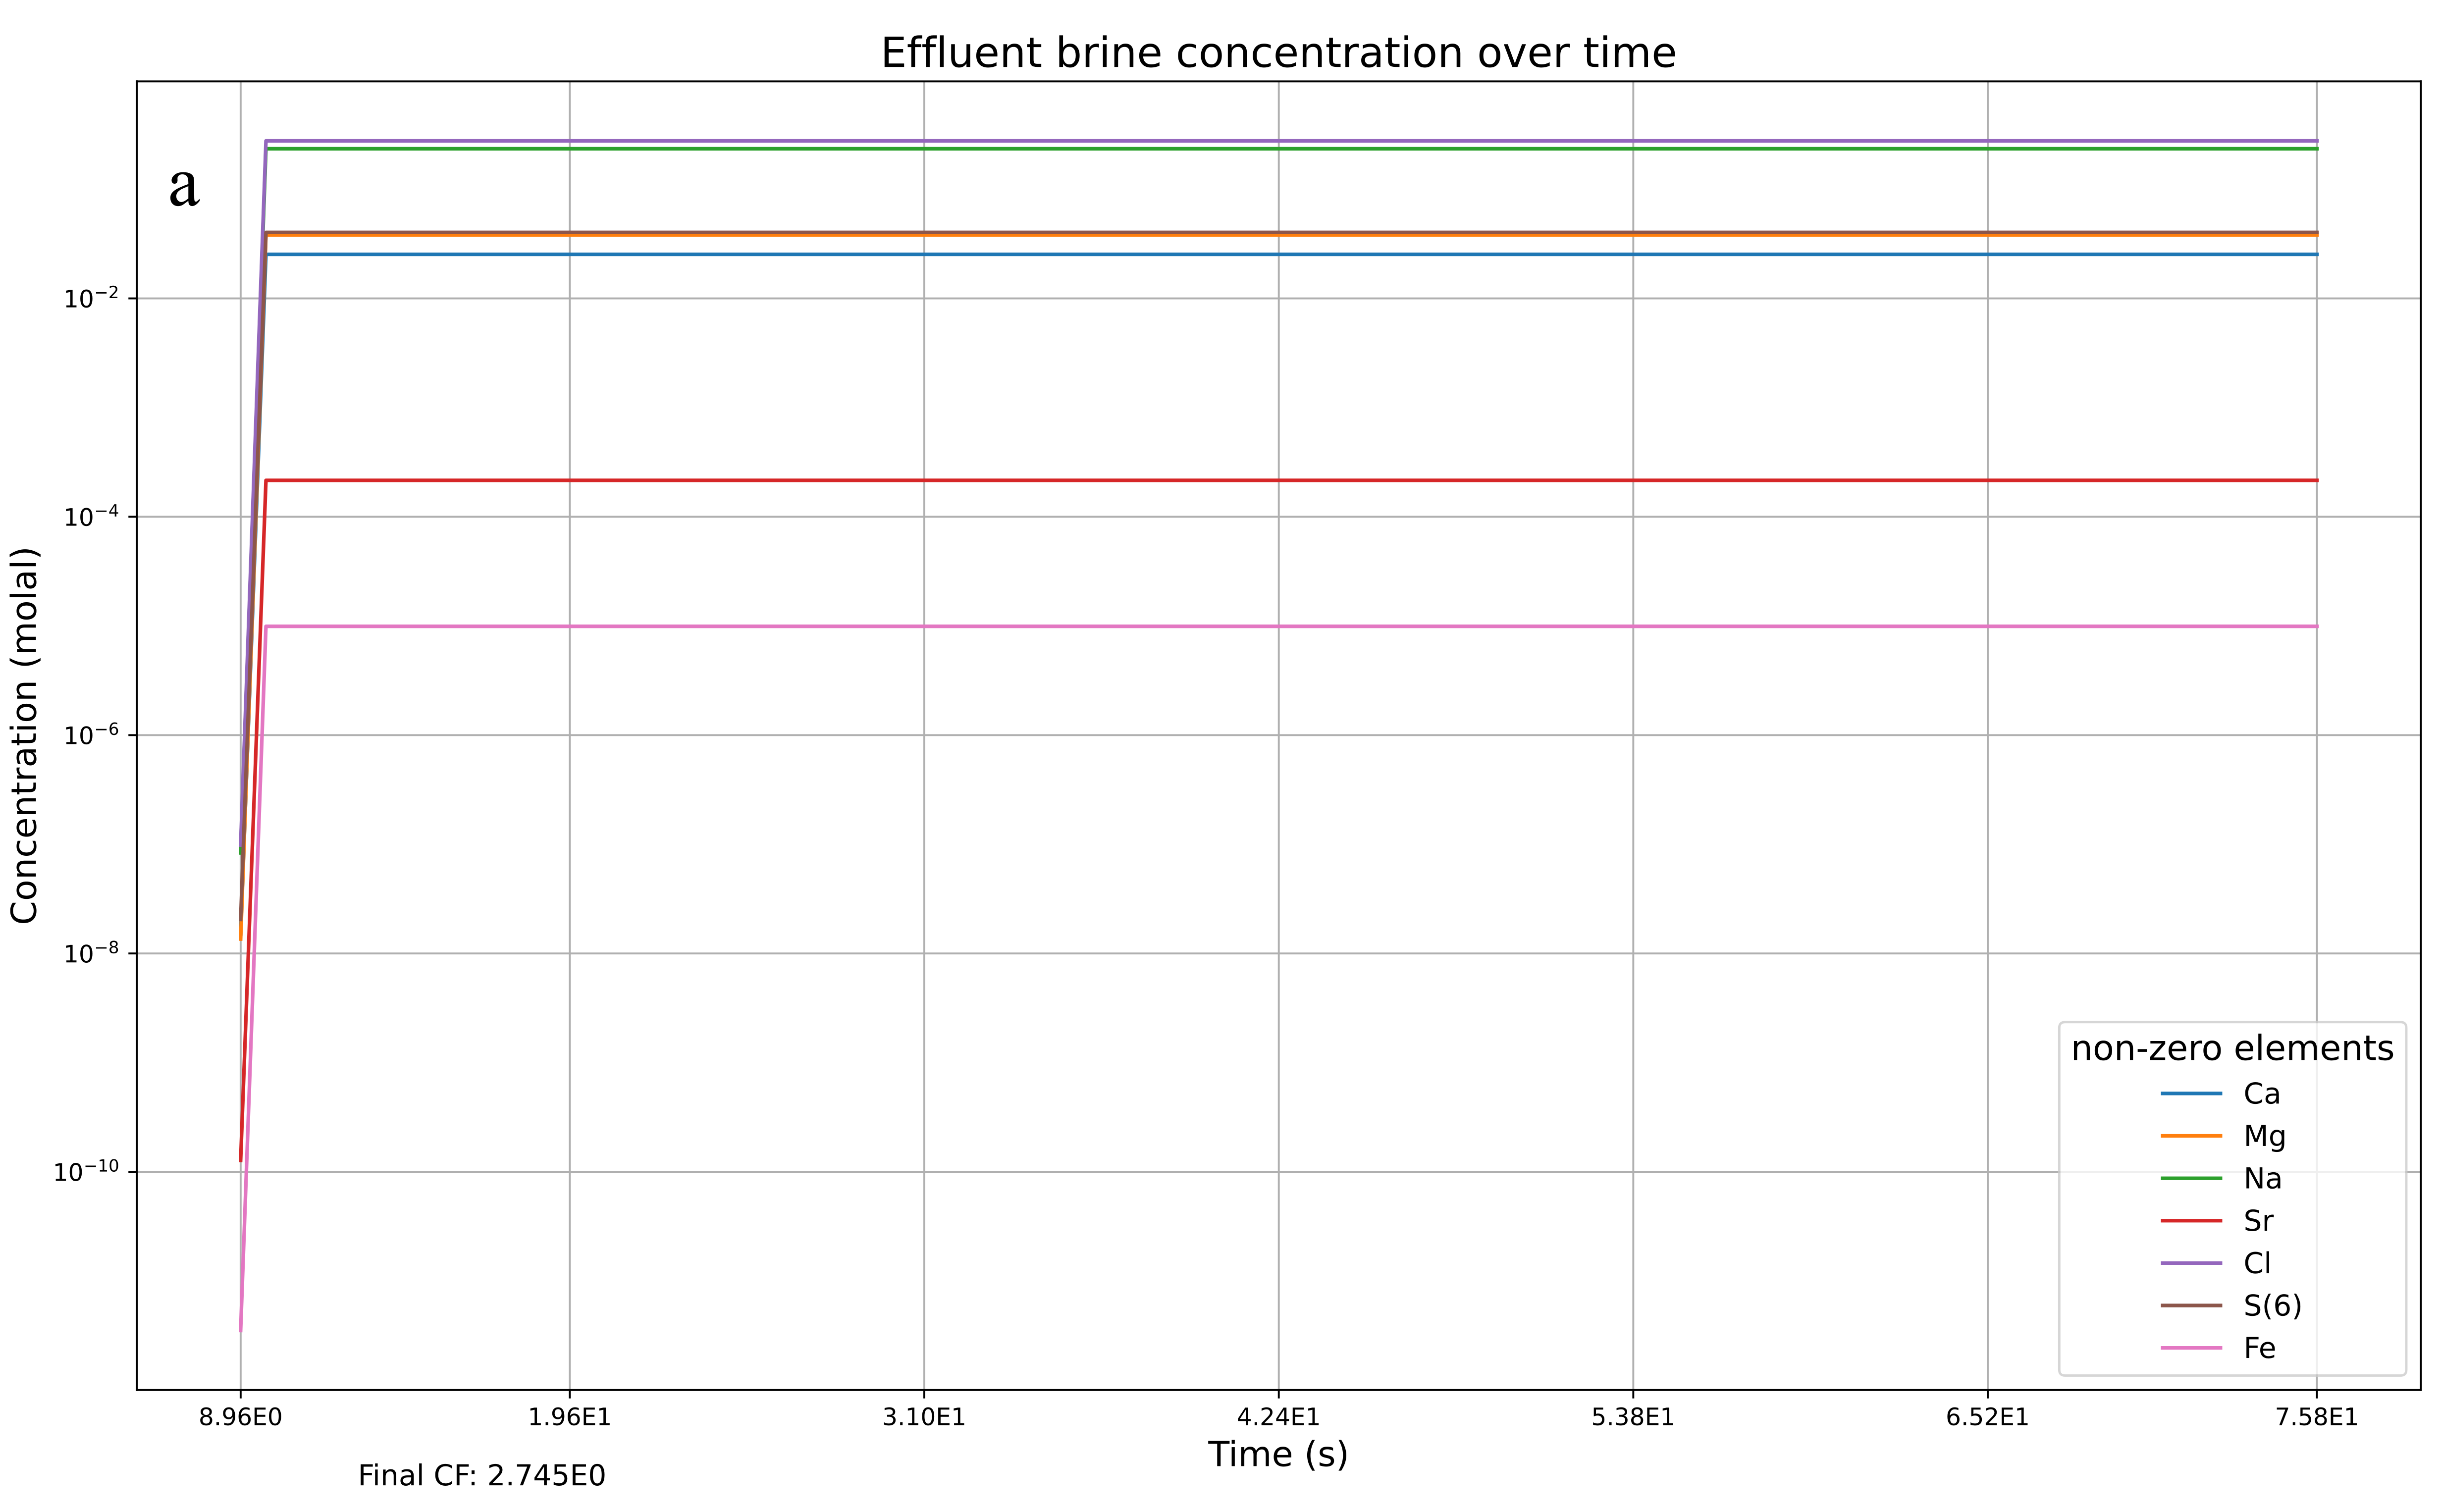
\includegraphics[width=\linewidth]{images/ROSSpy/sensitivity_analyses/simulation_perspective/brine_all_time.png} \\ \midrule
        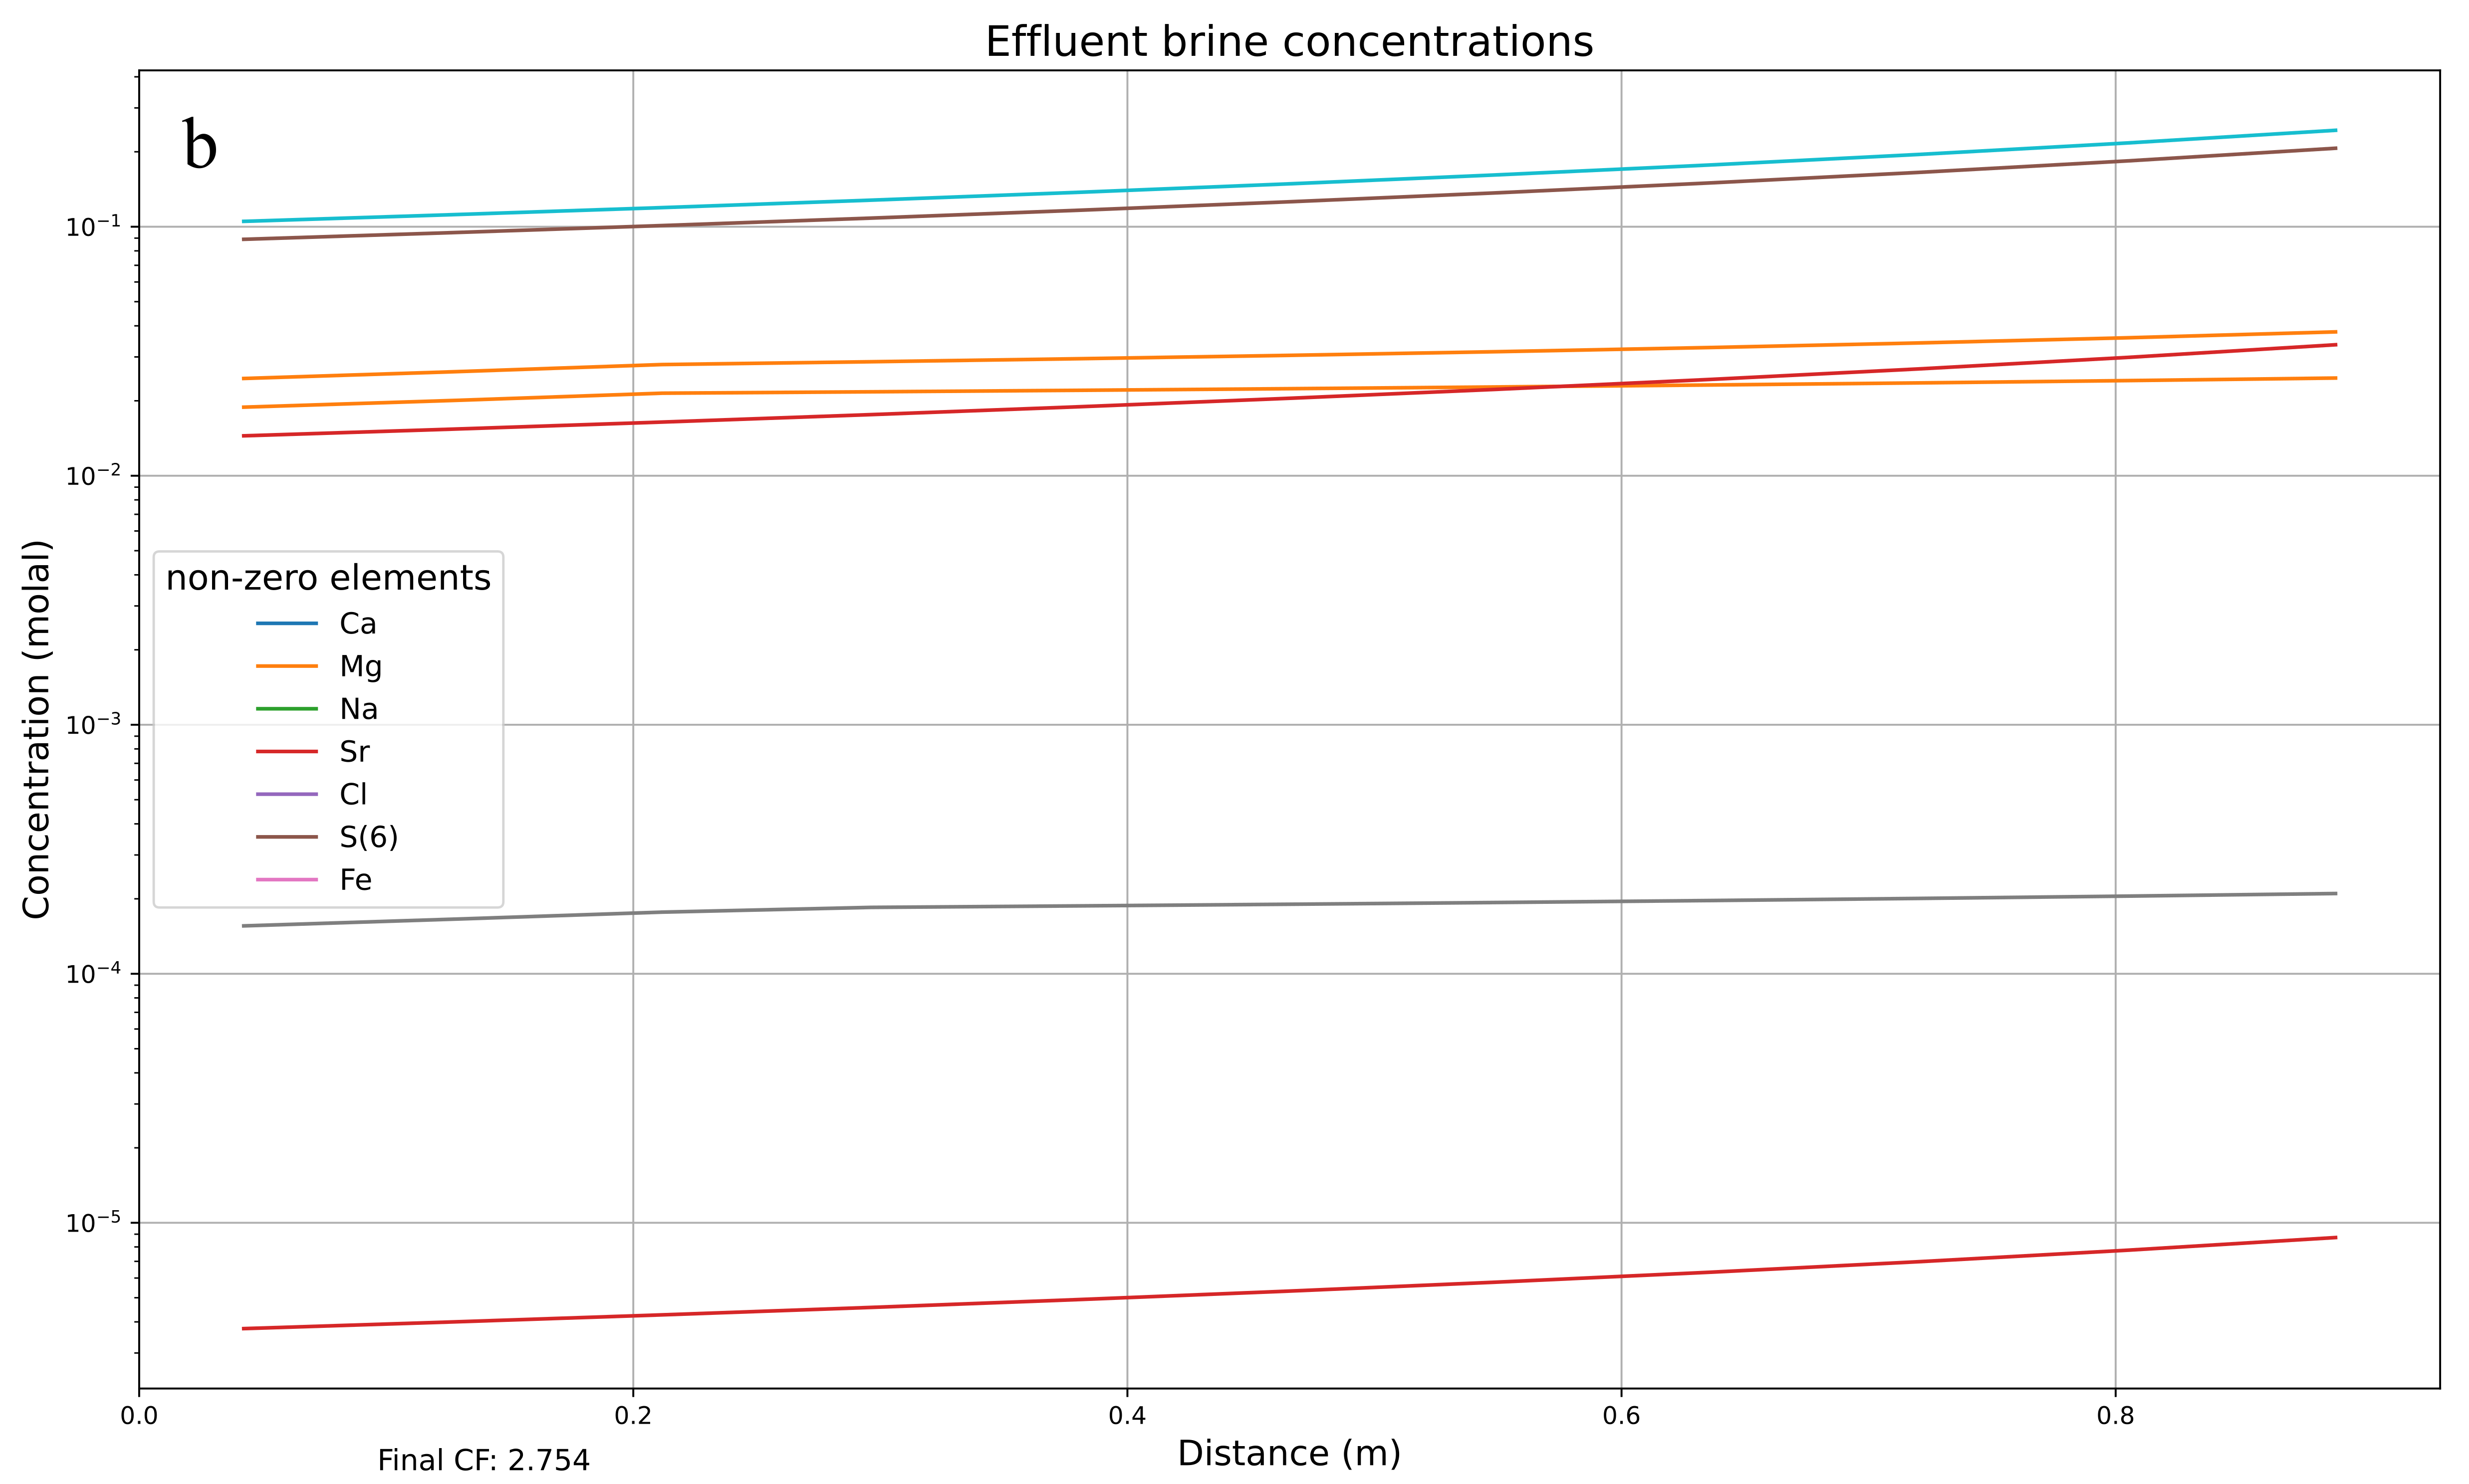
\includegraphics[width=\linewidth]{images/ROSSpy/sensitivity_analyses/simulation_perspective/brine_all_distance.png}
    \end{tabular}
    \caption{
        Brine formation while either a) slicing through time at the end distance or b) slicing  through distance at the final time. The final concentrations differ slightly between the two simulation perspectives, where the all\_time perspective calculates the true end of the last cell while the all\_distance perspective calculates the mid-point of the last cell and thus has a slightly lower concentration. 
    }
    \label{brine_perspectives}
\end{figure}

\begin{figure}[h]
    \centering
    \begin{tabular}{c}
        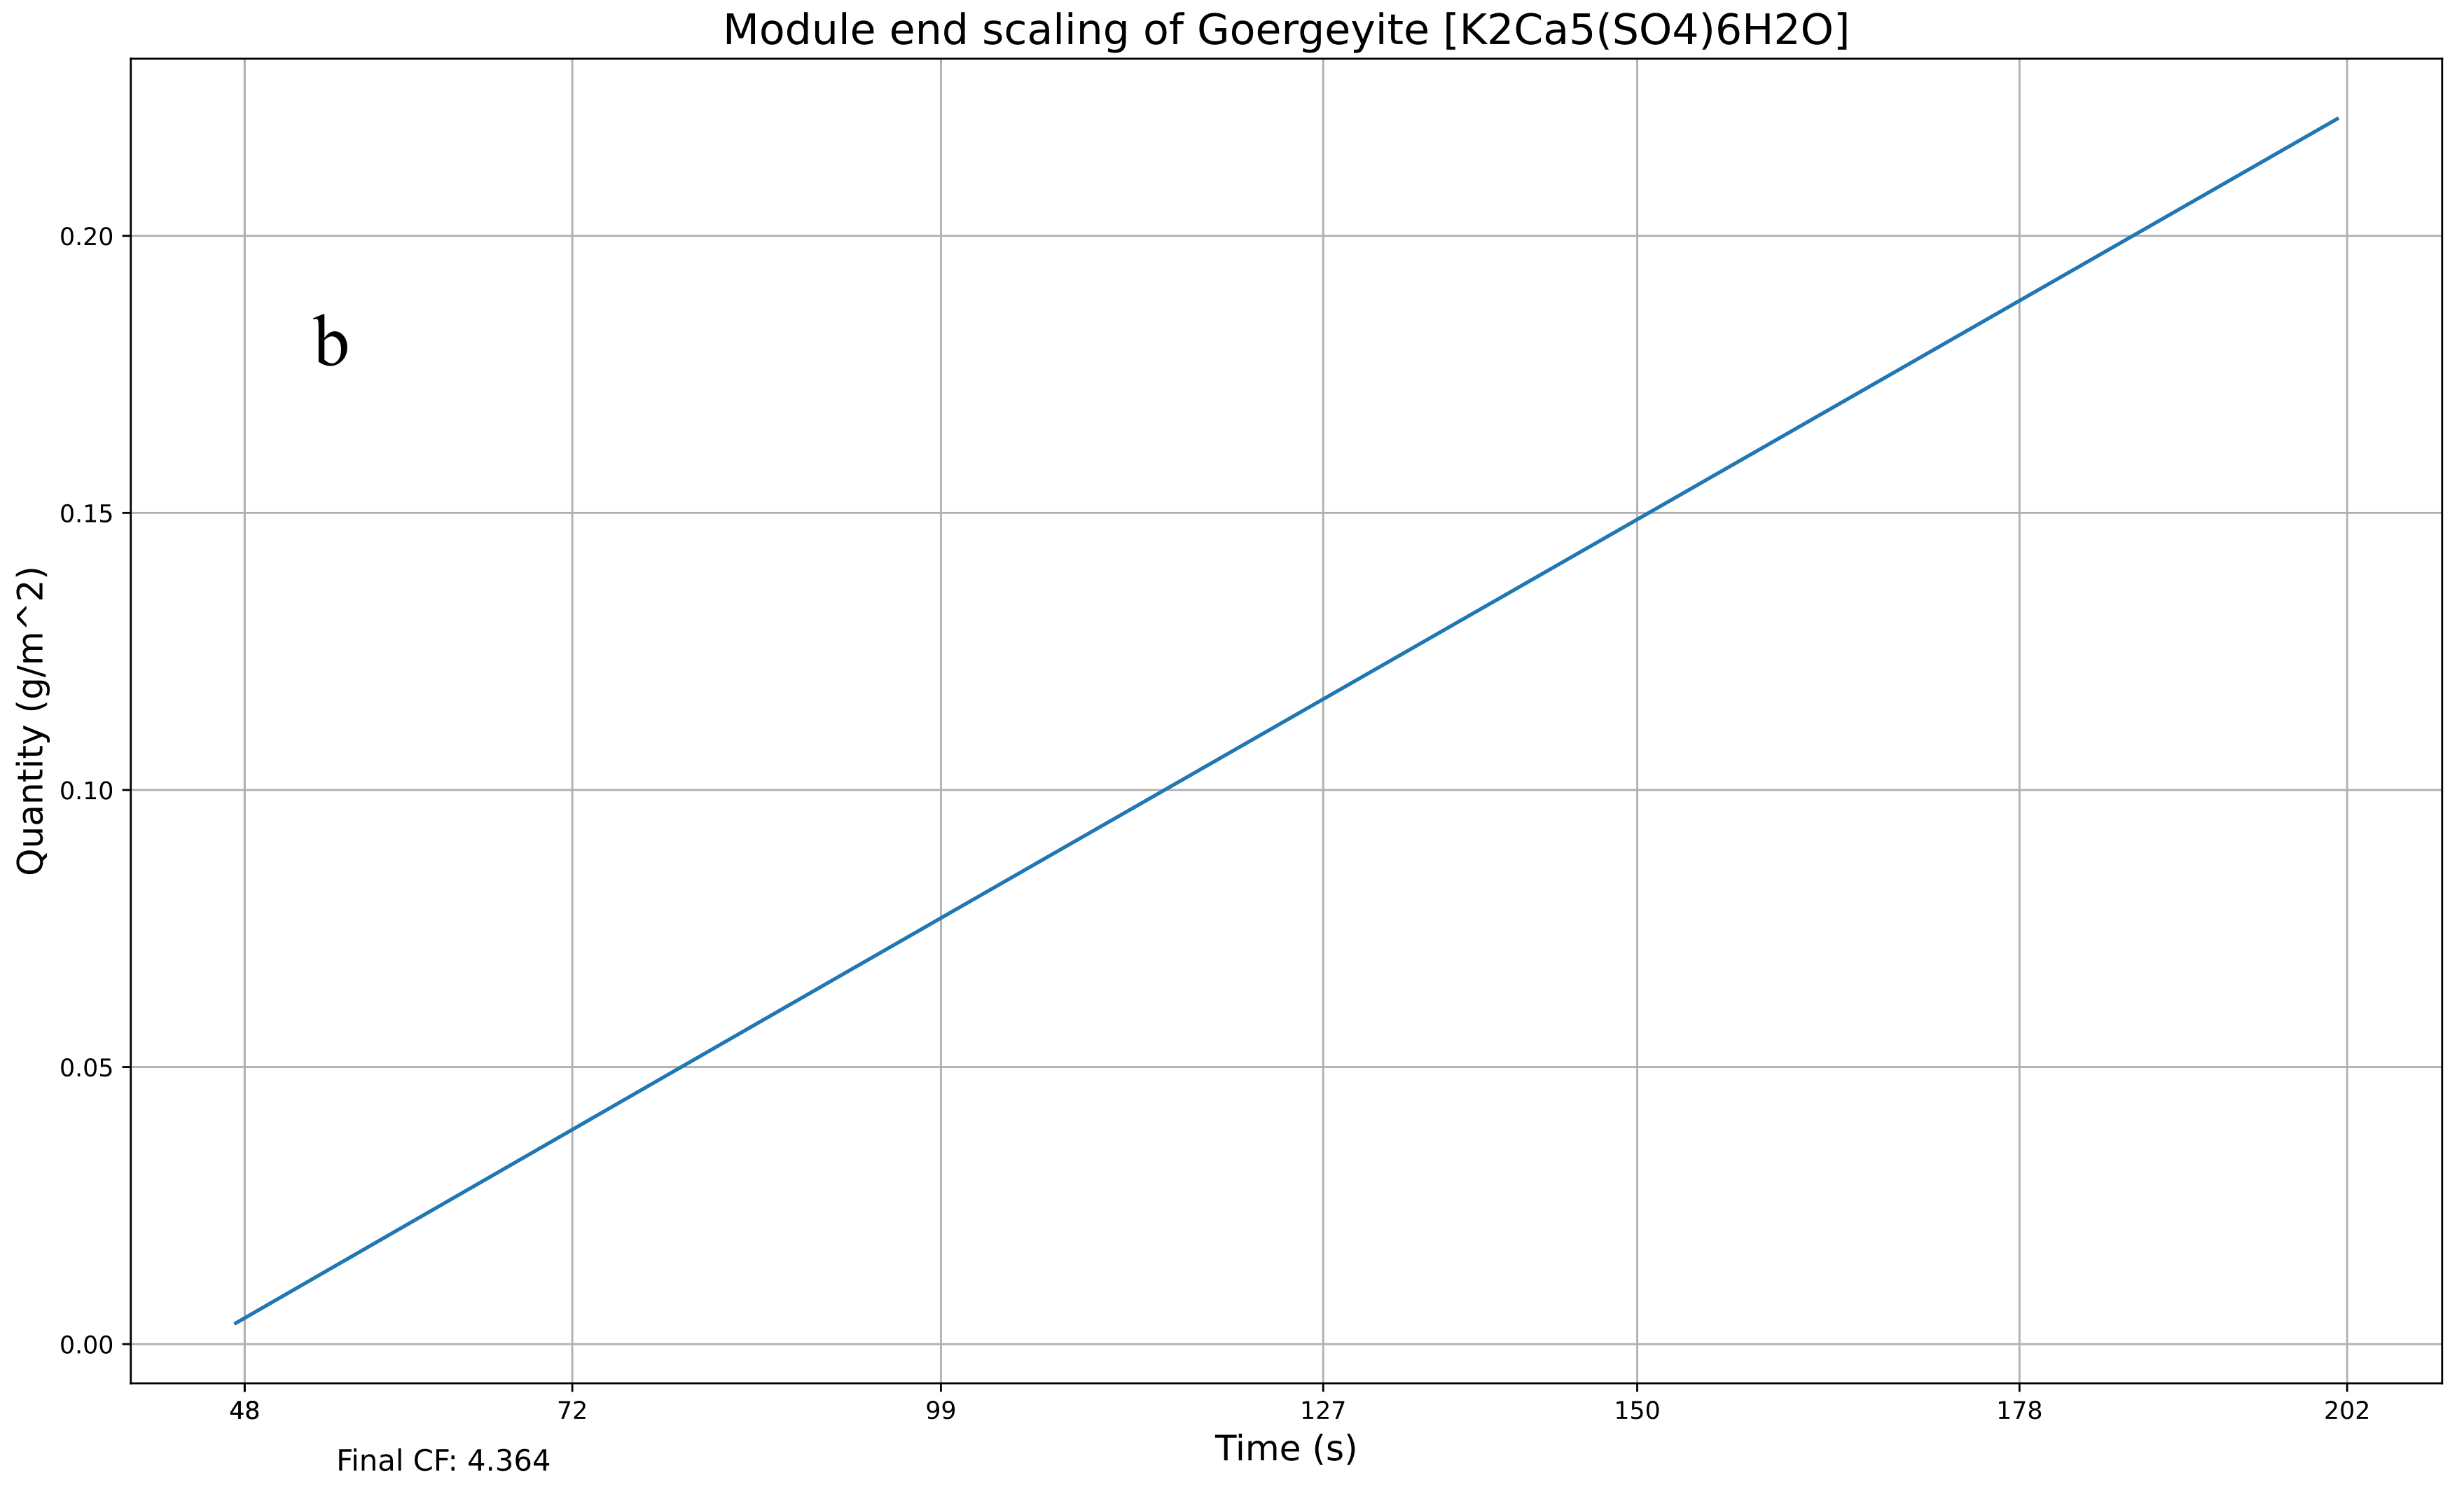
\includegraphics[width=\linewidth]{images/ROSSpy/case_studies/scaling_all_time_goergeyite.png} 
        \\ \midrule
        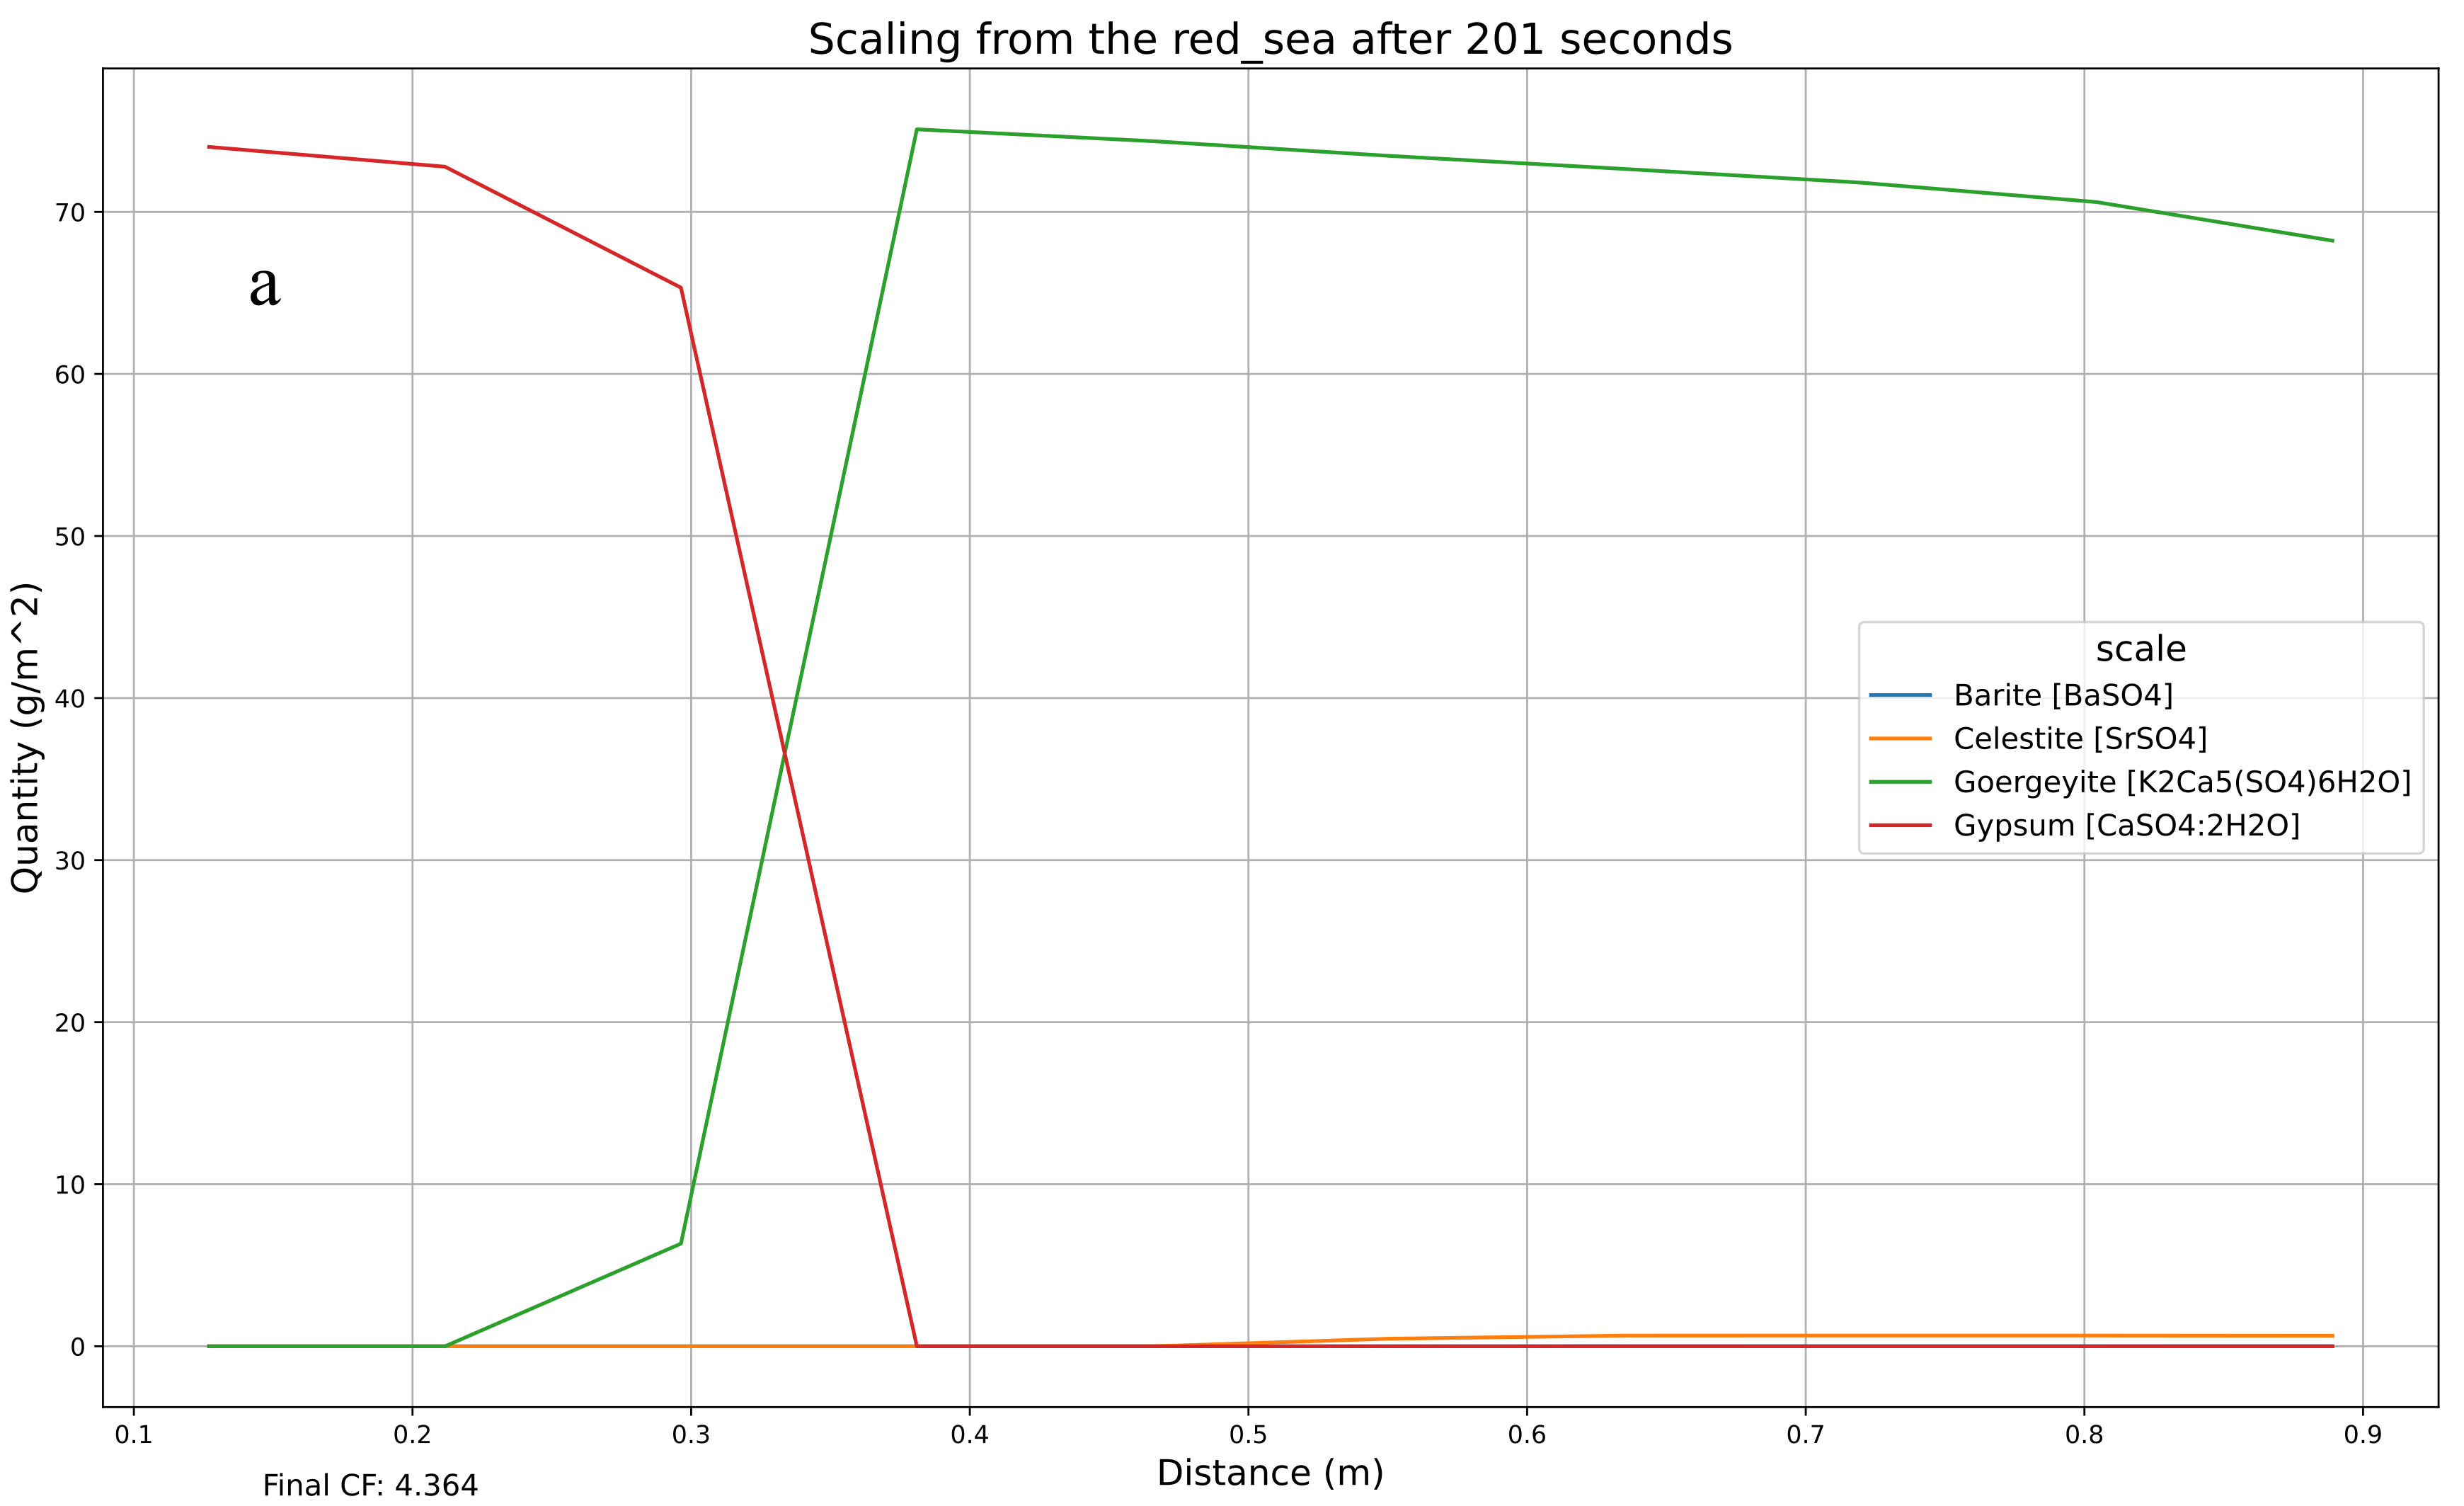
\includegraphics[width=\linewidth]{images/ROSSpy/case_studies/scaling_all_distance.png} 
    \end{tabular}
    \caption{
        Scaling while either a) slicing through time at the end distance or b) slicing  through distance at the final time. The permeate flux of the simulation is elevated to augment the scaling geochemistry for this illustration.
    }
    \label{scaling_perspectives}
\end{figure}

\subsection{Feed geochemistry}
Each of the default feed parameter files, including both natural seas and produced waters from oil wells, were evaluated with otherwise identical simulation parameters. The scaling and brine predictions differed significantly amongst these feed water sources, which are sampled in Figure \ref{feed_sources}.  

\begin{figure}[h]
    \centering
    \begin{tabular}{c|c}
        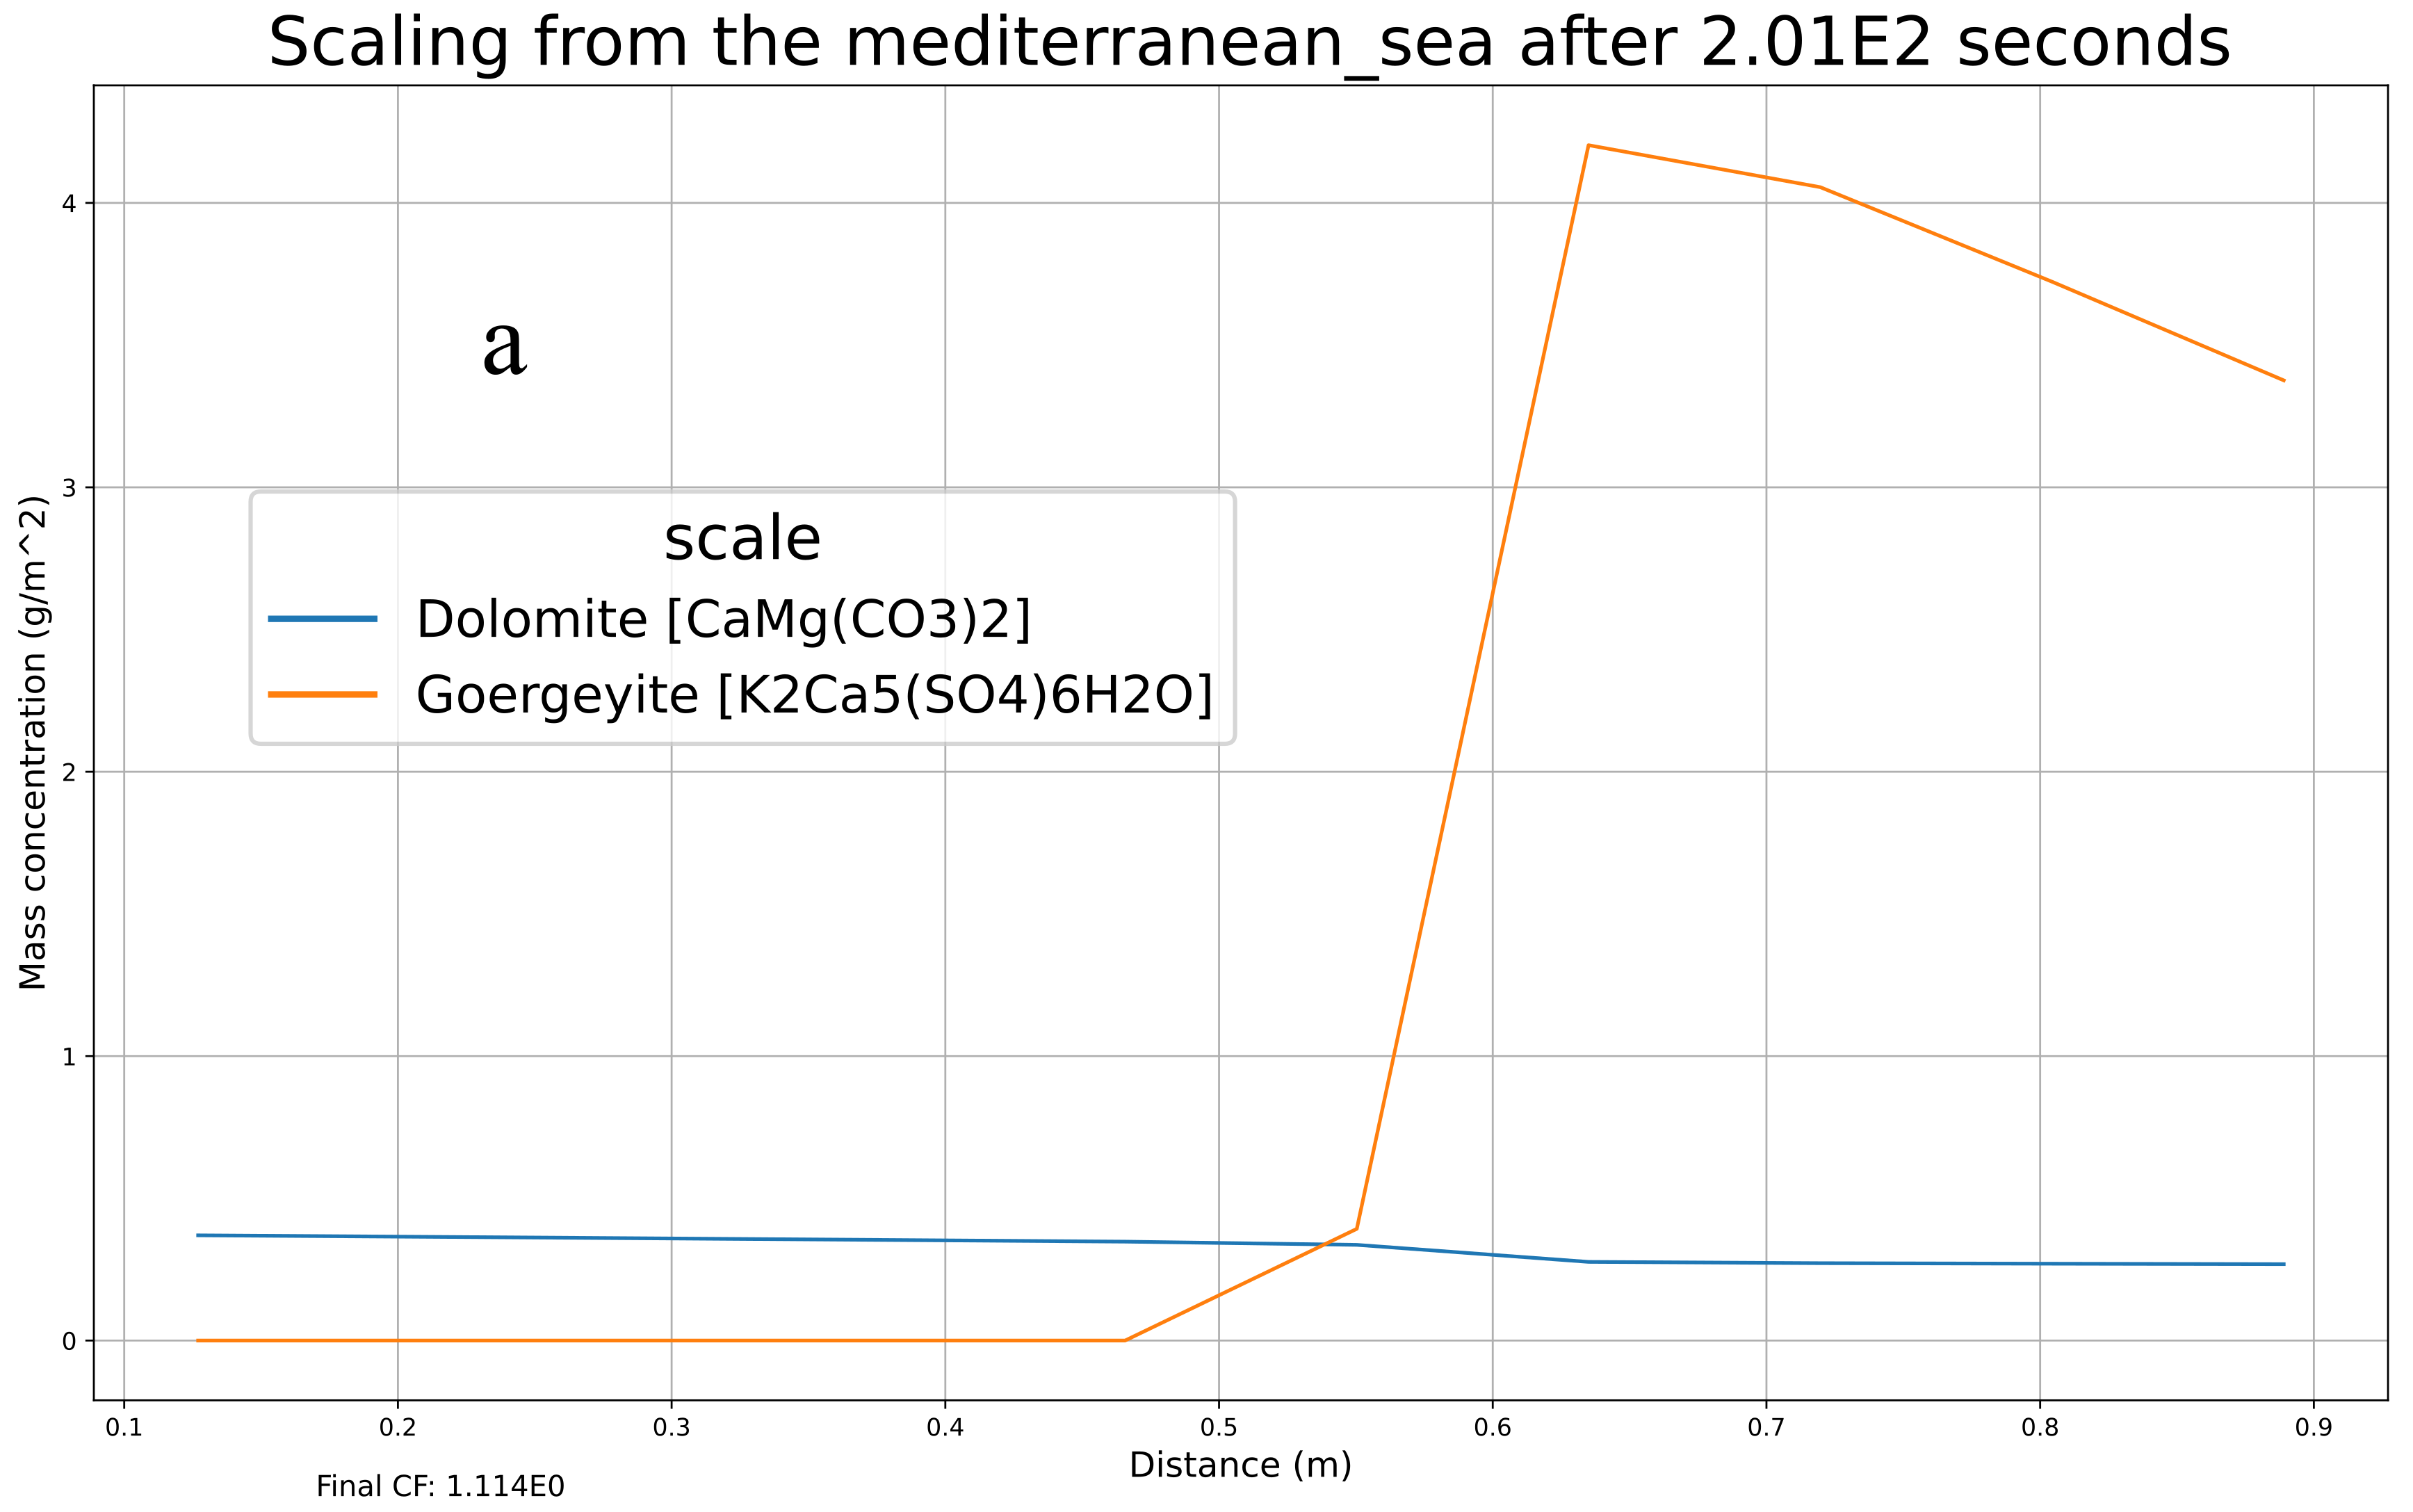
\includegraphics[width=0.49\textwidth]{images/ROSSpy/sensitivity_analyses/feed_source/Mediterranean.png} &
        \includegraphics[width=0.49\textwidth]{images/ROSSpy/sensitivity_analyses/feed_source/Palo_Duro_basin.png} \\ \midrule
        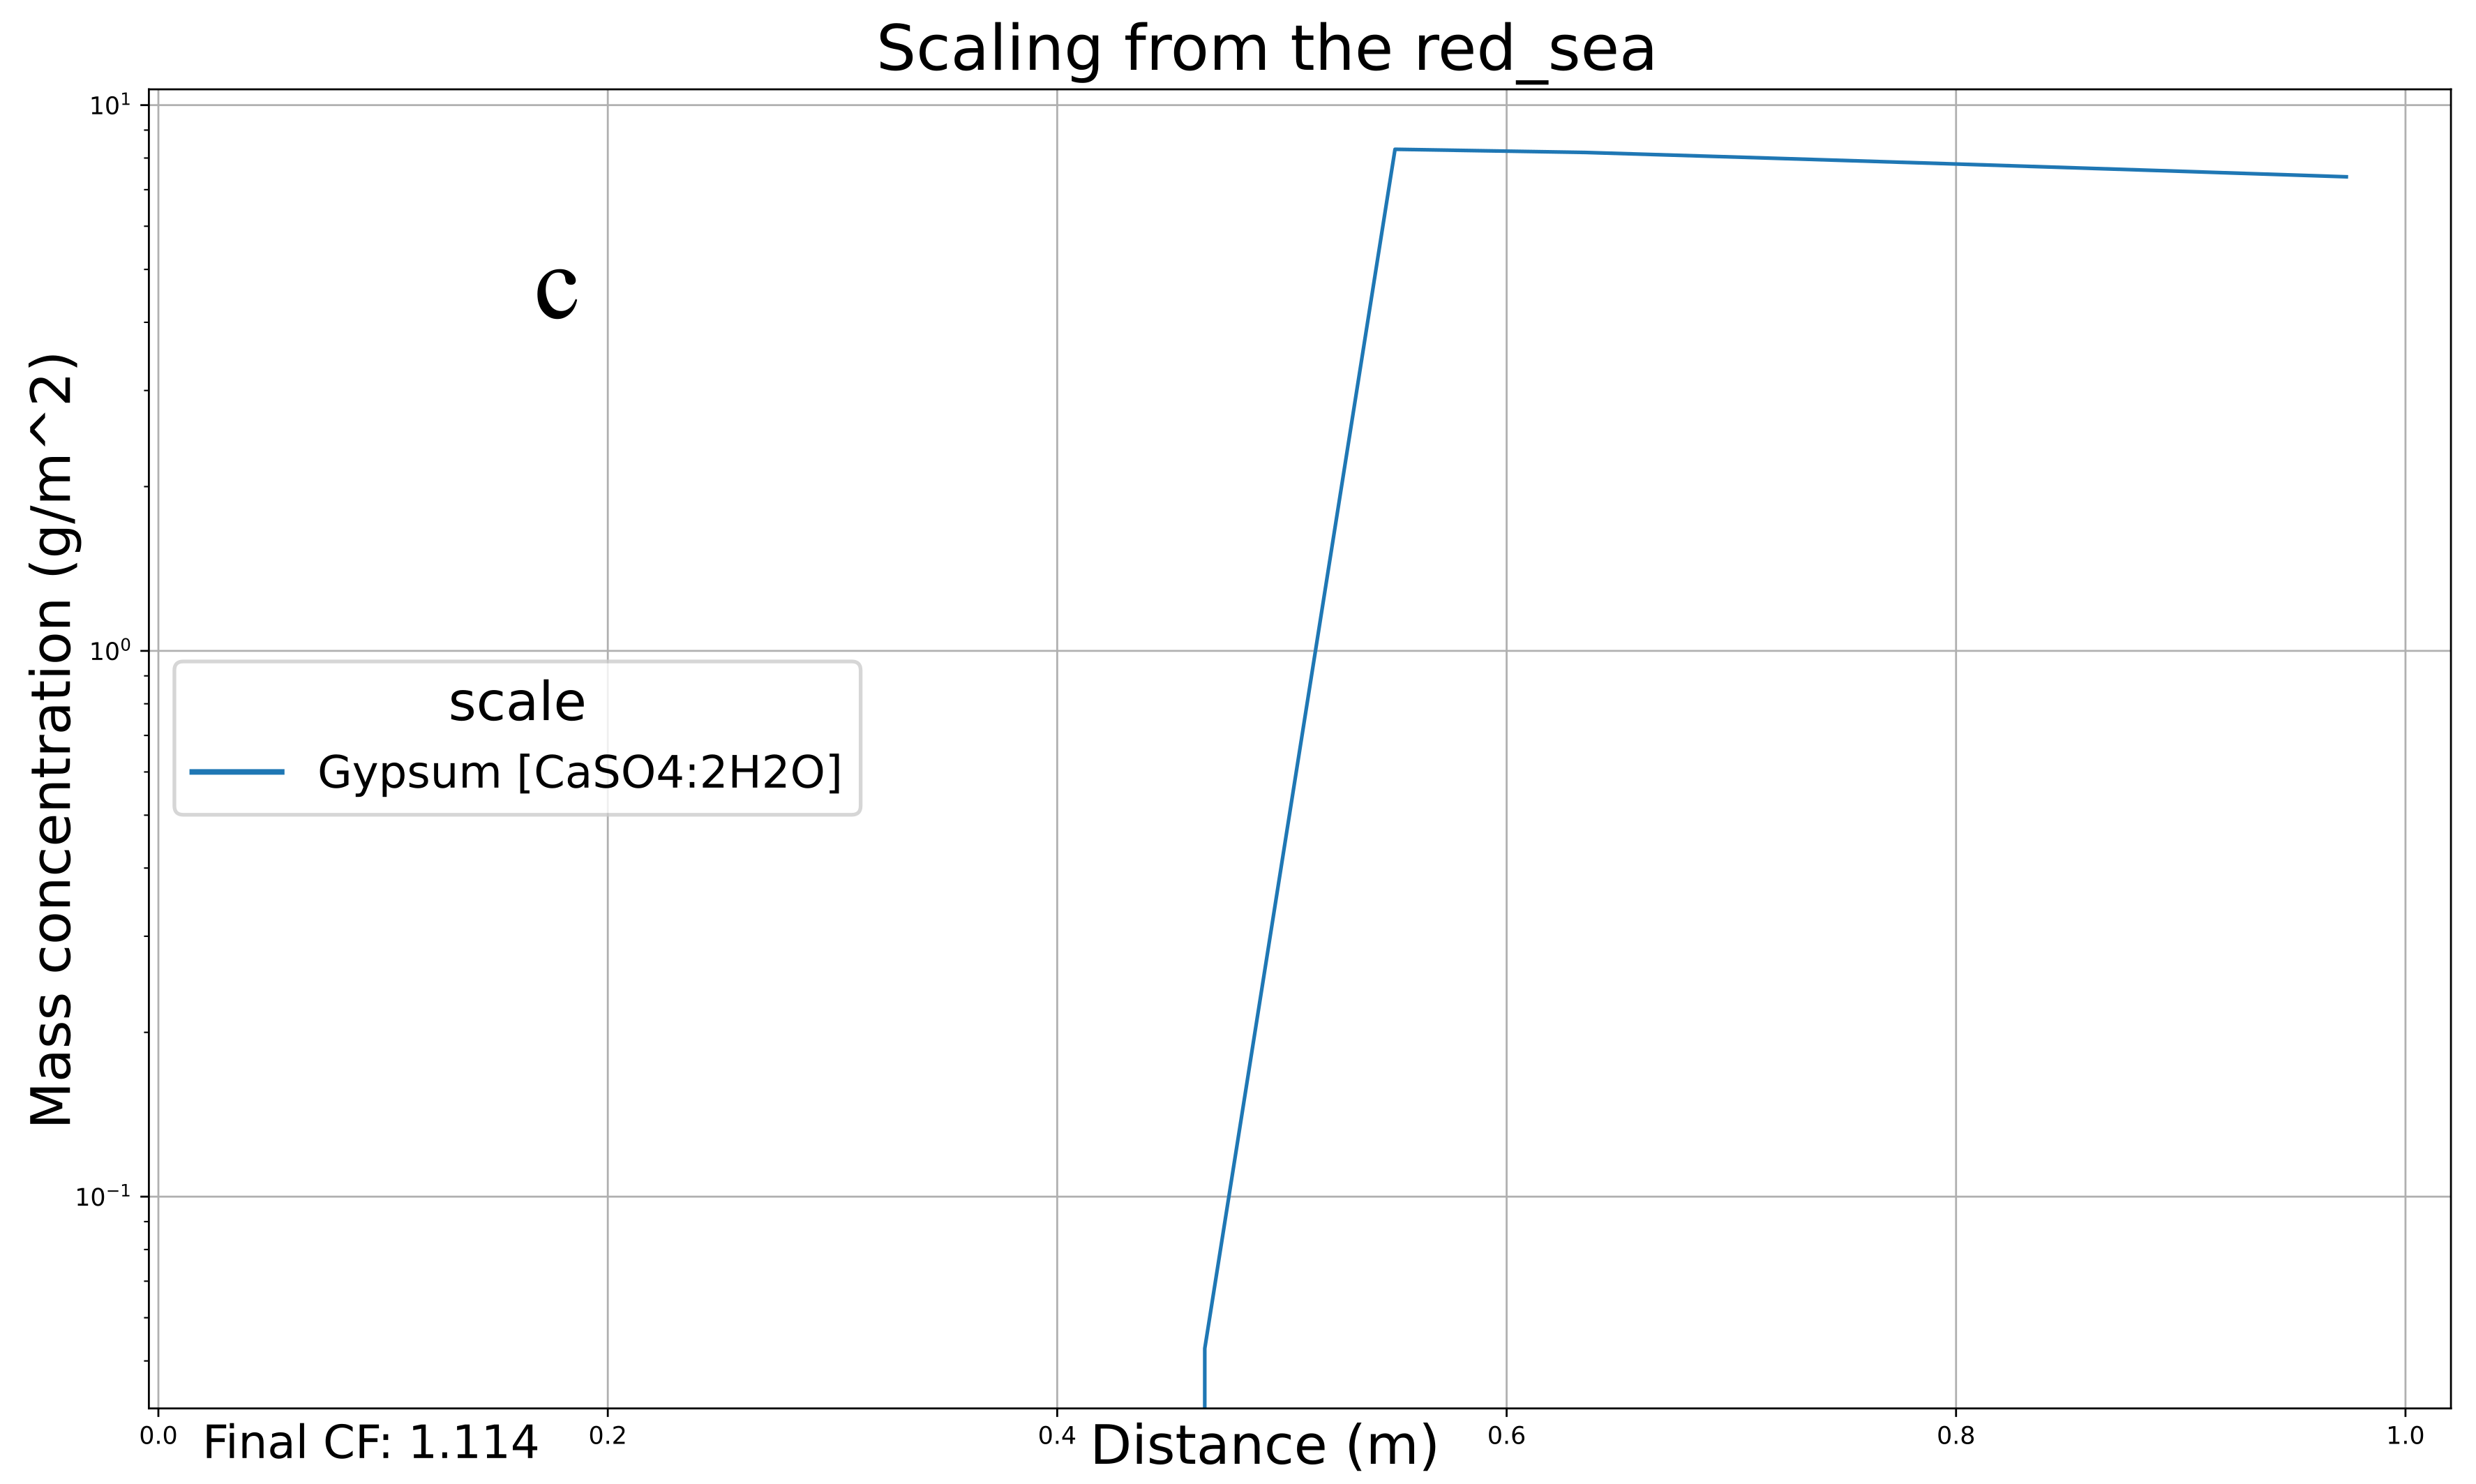
\includegraphics[width=0.49\textwidth]{images/ROSSpy/sensitivity_analyses/feed_source/Red_Sea.png} & 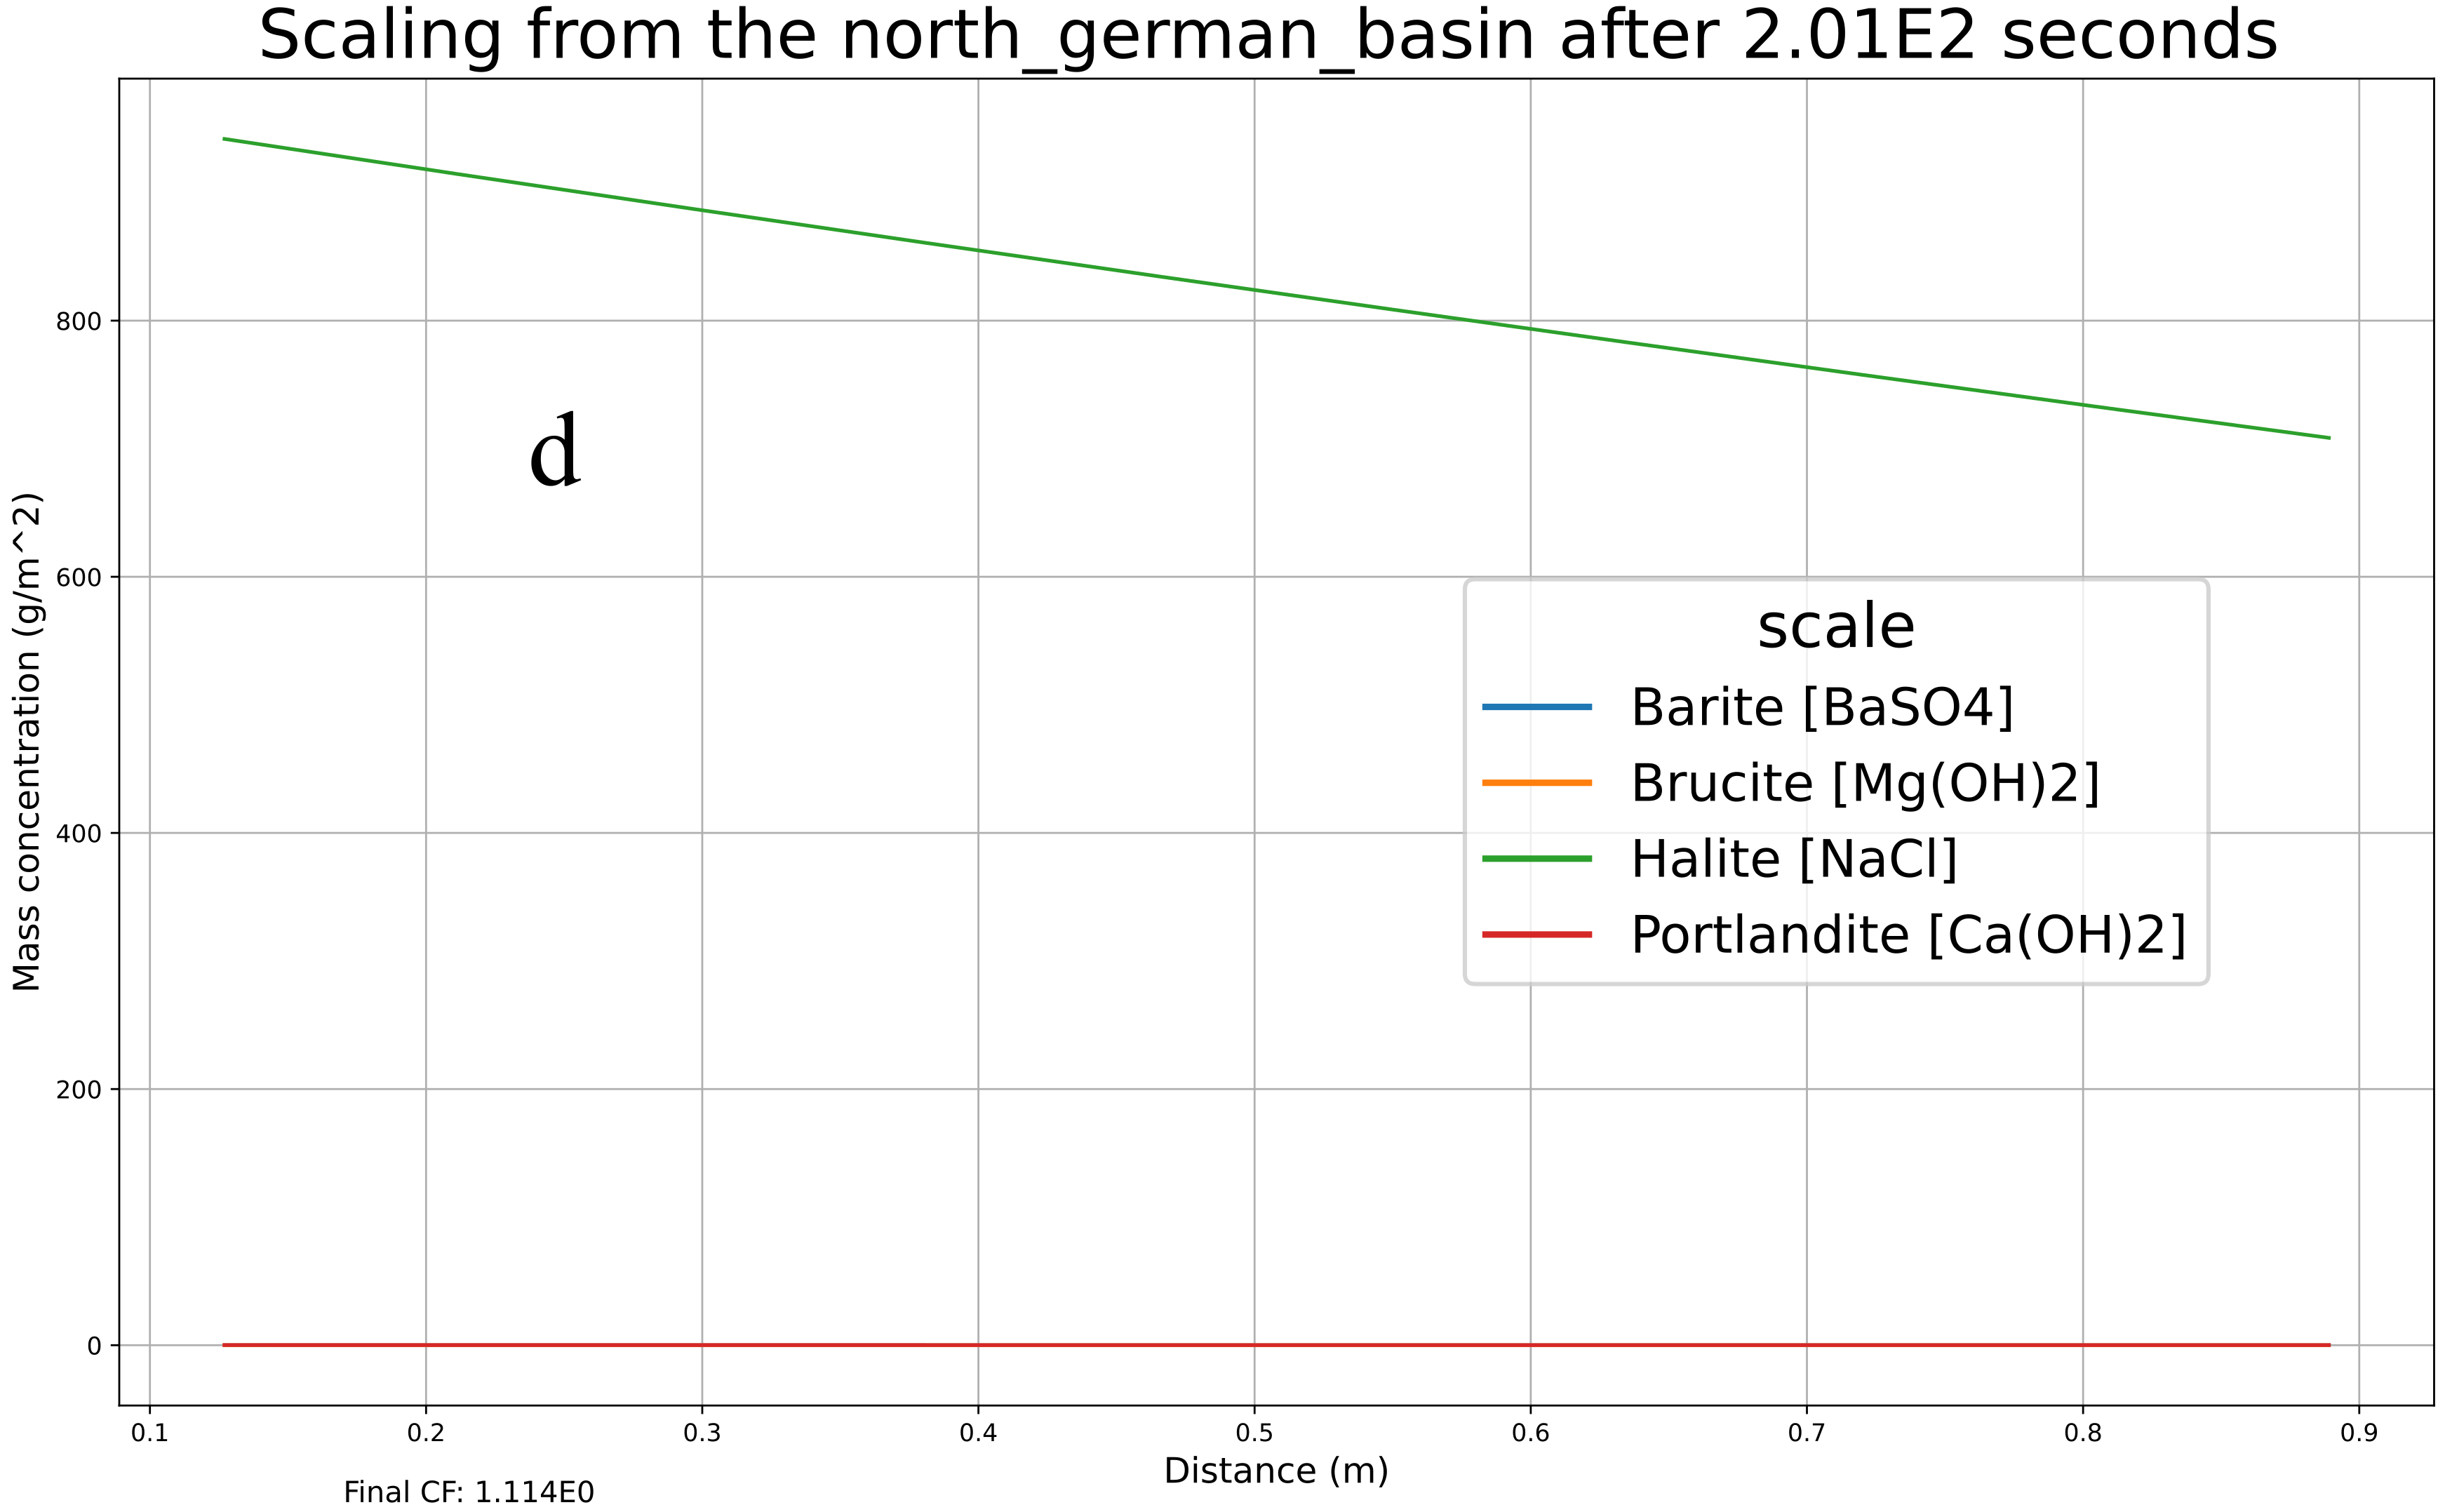
\includegraphics[width=0.49\textwidth]{images/ROSSpy/sensitivity_analyses/feed_source/German_Basin.png} \\ \bottomrule
    \end{tabular}
    \caption{
        Scaling predictions of a) the Mediterranean Sea, b) produced waters from the Palo Duro oil basin, c) the Red Sea, d) produced waters from the North German oil basin, with otherwise identical simulation parameters.
    }
    \label{feed_sources}
\end{figure}


\section{Conclusion}

A one-dimensional approximation of RO reactive transport geochemistry, modeled in PHREEQC, is a practical and accurate approach of representing mineral scaling from RO desalination. A range of simulation applications of this model, and quantitatively and qualitatively assessment of the simulation predictions, were verified through its implementation as a Python API: ROSSpy. The light-weight program is furthermore tenable for personal computers, accessible through common coding languages, and open-source for community involvement and improvement. We expect that these unique attributes of the one-dimensional model and the ROSSpy software -- e.g. rapidly designing, executing, processing, and exporting RO simulations -- will facilitate scaling research and ultimately improve the efficiency of RO desalination towards alleviating water insecurities around the world. 


\section{Funding}
This work was prepared in partial fulfillment of the requirements of the Berkeley Lab Undergraduate Research (BLUR) Program, managed by Workforce Development \& Education at the Berkeley Lab. The project was also partly funded by NSERC Discovery, MITACS Accelerate, CEWIL, and Canada Summer Jobs. 

% \bibliography{mendeley_references.bib}